% !TeX program = xelatex
%this will be based on the amsart class, which probably causes more pain than necessary
%but gets a lot of the formatting the way I like it
%look for !!!EDIT comments
\documentclass[reqno,oneside,12pt]{amsart}
% \usepackage[T1]{fontenc}
\usepackage{fontspec}
\setmainfont{Times New Roman}
\usepackage{amsmath,amsfonts,amsthm,amssymb} %provides all math symbols etc.
%graphics
\usepackage{graphicx}
\usepackage{wrapfig}
\usepackage[margin=0.1cm,textfont=it]{caption}
%set 1" margins:
\usepackage[left=1in,top=1in,right=1in,bottom=1in,footskip = 0.333in]{geometry}
%provide additional table capability
\usepackage{tabularx}

\usepackage{pdfpages}
\usepackage{multirow} 
%eqution
\everydisplay{\setlength{\abovedisplayskip}{10pt}\setlength{\belowdisplayskip}{10pt}}
%subsubsection
%\usepackage{titlesec}
%\titlespacing*{\subsubsection}{0pt}{10pt}{10pt}

\usepackage{titletoc}
\usepackage{subfig}
\usepackage{xcolor} % 用于设置表格颜色
\usepackage{array}         % 用于更灵活的列定义
\usepackage{booktabs}      % 用于更好的表格线
\usepackage{colortbl}
% \setcounter{tocdepth}{4}
% \setcounter{secnumdepth}{3}
\usepackage{makecell}
\usepackage{wrapfig}%
\usepackage{comment}
\usepackage[utf8]{inputenc}
\usepackage{indentfirst}
\usepackage{enumitem}
\usepackage{listings}

% 定义黄色背景颜色
\definecolor{myyellow}{RGB}{255, 255, 0}
\definecolor{lightgray}{rgb}{0.9, 0.9, 0.9}
\definecolor{diffgreen}{rgb}{0.0, 0.6, 0.0}
\definecolor{commentteal}{rgb}{0.13, 0.55, 0.51}
\definecolor{codegray}{rgb}{0.5, 0.5, 0.5} 

% 设置自动换行并居中对齐
\newcolumntype{C}[1]{>{\centering\arraybackslash}p{#1}}
\newcolumntype{L}[1]{>{\raggedright\arraybackslash}p{#1}}



\numberwithin{equation}{section}

\lstdefinestyle{pythonstyle}{
    language=Python,
    basicstyle=\ttfamily\small,            % 等宽字体，字号偏小
    commentstyle=\color{commentteal}\itshape, % 注释：青色 + 斜体
    keywordstyle=\bfseries,                % 关键字：加粗
    stringstyle=\color{black},             % 字符串颜色
    numberstyle=\tiny\color{codegray},     % 左侧行号：极小字号 + 灰色
    numbers=left,                          % 行号显示在左侧
    numbersep=12pt,                        % 行号与代码的距离
    frame=tb,                              % 重点：在代码块顶部 (t) 和底部 (b) 绘制横线
    rulecolor=\color{black},               % 横线颜色
    breaklines=true,                       % 自动换行
    showstringspaces=false,                % 不显示字符串中的空格标记
    tabsize=4
}
\lstset{style=pythonstyle}

\usepackage{cite}





\begin{document}
\begin{center}
\textbf{ASC 2026 Proposal of XTU}\\  %!!!EDIT
\end{center}

\begin{flushleft}
  \textsl{Team members: Huayu Shen, Yangkun Pei, Long Jiang, Muyuan Chen, Tao Li}

  \textsl{Advisor: Peiying Lin}
\end{flushleft}


\titlecontents{section}[0pt]{\vspace{0.25em}\bfseries}{\contentslabel{0.1em}}{\hspace*{0.5em}}{\titlerule*[0.5pc]{.}\contentspage}
\titlecontents{subsection}[0pt]{\vspace{0.25em}}{\contentslabel{0.1em}}{\hspace*{1.5em}}{\titlerule*[0.5pc]{.}\contentspage}
\titlecontents{subsubsection}[0pt]{\vspace{0.25em}}{\contentslabel{0.1em}}{\hspace*{2.5em}}{\titlerule*[0.5pc]{.}\contentspage}
\setcounter{tocdepth}{3}

\tableofcontents
\clearpage



%important---今年新要求：最多不超过3页
\section{Supercomputing Activities}
% 湘潭大学是一所享有盛誉的综合性全国重点大学及国家“双一流”建设高校，巍然屹立于伟大领袖毛泽东主席的故乡——湘潭。湘潭大学不仅具备现代化的教学设施，还配备了先进的高性能计算中心。在高性能人才培养方面，学校为学生提供丰富的高性能学习资源，涵盖前沿的专业课程、高水平的学术讲座、创新的研究项目以及强大的高性能计算平台等。这些资源不仅拓宽了学生的视野，也为他们提供了坚实的学术和技术支持。去年首次参加了ASC比赛，虽然没能进入决赛，但46的排名让学生们备受鼓舞，学校也给予了高度认可。接下来，我们将介绍学校(的超算平台和超算相关活动。
Xiangtan University(XTU) is a prestigious comprehensive national key university and a ``Double First-Class" construction university of the country. 
Standing majestically in the hometown of the great leader Mao Zedong, XTU is a place of great renown. 
XTU not only has modern teaching facilities, but also is equipped with an advanced high-performance computing center. 
In terms of high-performance talent cultivation, the school provides students with abundant high-performance learning resources, including cutting-edge professional courses, high-level academic lectures, innovative research projects, and a powerful high-performance computing platforms. 
These resources not only broaden students' horizons, but also provide them solid academic and technical support. 
Last year, we participated in the ASC competition for the first time. 
Although we didn't make it to the finals, our ranking of 46th was very encouraging for the students, and the school also gave us high recognition.
Next, we will introduce the university's supercomputing platform and supercomputing-related activities.

\subsection{The HPC Platform of XTU}
\ 
% 湘潭大学超级异构并行计算集群是省财政重点支持的“十四五”新基建重点项目，集群包含ClusterEngine高性能计算平台和AIstation人工智能平台，面向全校师生开放。集群计算能力为总浮点峰值性能为509万亿次的CPU双精度理论计算能力（6112个物理核心）和1552万亿次的GPU单精度理论计算能力。集群总体逻辑框架设计图如图所示。

% ClusterEngine高性能计算平台包含1台管理节点，1台登录节点，1台物理监控平台，85个通用计算节点，2个大内存计算节点，共5472个CPU核心，内存总容量44.5TB，节点间通过千兆以太网和Infiniband相互连接。
% 管理、登录节点配置16个CPU核心，64G内存。
% 集群总共有两个资源分区，分别是CU、FAT分区。
% CU分区配置80台通用计算节点，每台计算节点分别配置64个Intel 8358 CPU核心，512G内存；80台cpu计算节点共5120个CPU核心。
% FAT分区配置2台大内存计算节点，每台节点配置16个intel 6334 CPU核心，1TB内存。
% 平台的主要功能是面向全校提供高性能科学与工程计算服务，满足各学科领域对于大规模数据处理和大规模科学计算的需求。平台主要应用领域包括：数学、统计学、力学、物理学、化学、化学工程、生物学、地球科学、航天航空科学技术、计算机科学等多学科提供高性能计算环境。
% 平台提供Intel MKL 2020、FFTW3 3.10、Openblas、Blas等数学库以及Intel MPI 2020、OpenMPI、Mpich等并行环境。支持丰富的应用软件，如MATLAB，OpenFOAM，ABINIT，GROMACS，NAMD等。

% AIstation人工智能平台共包含10个GPU计算节点，共640个CPU核心，80块NVIDIA A100 加速卡，内存总容量5TB，并行存储与高性能计算平台共用，总容量1.3PB，GPU 实测峰值速度可以达到每秒888.9万亿次。


Xiangtan University's Super Heterogeneous Parallel Computing Cluster is a key project supported by the provincial finance under the ``4th Five-Year Plan" for new infrastructure construction. 
The cluster includes ClusterEngine high-performance computing platform and AIstation artificial intelligence platform, and is open to all teachers and students of the university. 
The computing capacity of the cluster is the theoretical computing capacity of 509 trillion times of CPU double-precision peak performance (6,112 physical cores) and 1552 trillion times of GPU single-precision theoretical computing capacity.
The overall logical framework design diagram of the cluster is shown in the figure.

The ClusterEngine high-performance computing platform consists of 1 management node, 1 login node, 1 physical monitoring platform, 85 general-purpose computing nodes, 2 large-memory computing nodes, totaling 5472 CPU cores and a total memory capacity of 44.5TB. 
The nodes are interconnected through Gigabit Ethernet and Infiniband.
The management and login nodes are each equipped with 16 CPU cores and 64GB of memory.

The cluster has two resource partitions: CU and FAT partitions. 
The CU partition is configured with 80 general-purpose computing nodes, each with 64 Intel 8358 CPU cores and 512GB of memory, totaling 5,120 CPU cores. 
The FAT partition is configured with 2 large-memory computing nodes, each with 16 Intel 6334 CPU cores and 1TB of memory. 


The main function of the platform is to provide high-performance scientific and engineering computing services to the entire university, meeting the needs of various disciplines for large-scale data processing and large-scale scientific computing. 
The platform's main application areas include providing high-performance computing environments for mathematics, statistics, mechanics, physics, chemistry, chemical engineering, biology, earth science, aerospace science and technology, computer science, and many other disciplines.
The platform supports a wide range of application software, such as MATLAB, OpenFOAM, ABINIT,GROMACS, NAMD and so on.

The AIstation artificial intelligence platform consists of 10 GPU computing nodes, with a total of 640 CPU cores, 80 NVIDIA A100 acceleration cards, a total memory capacity of 5TB, and shared with the parallel storage and high-performance computing platform. 
The total capacity is 1.3PB. 
The GPU's measured peak speed can reach 888.9 trillion operations per second. 
This platform supports single-machine and distributed running of mainstream AI frameworks as well as task visualization.

\subsection{HPC Activities}
\ 


% 湘潭大学积极开展与超算相关的学术活动和科研项目。例如，2022年6月，国家超级计算长沙中心副主任彭绍亮教授在湘潭大学作《基于超算的元宇宙算力与应用展望》的学术报告。此外，学校还参与了湖南算力网络融合协同创新平台的建设，推动算力基础设施互联组网和算力资源的高效利用。
%学校对ASC超算比赛大力支持，去年的超算比赛获奖后，学校官网、学校学生工作部公众号平台和湖南日报都做了相应宣传。
% 通过这些超算平台和相关活动，湘潭大学不仅为学生提供了丰富的学习资源，还助力学校在高性能计算领域的科研创新和人才培养。
Xiangtan University actively conducts academic activities and research projects related to supercomputing. 
For instance, in June 2022, Professor Peng Shaoliang, the deputy director of the National Supercomputing Changsha Center, delivered an academic report titled ``Prospects of Computational Power and Applications of the Metaverse Based on Supercomputing" at Xiangtan University. 
Moreover, the university has participated in the construction of the Hunan Computing Power Network Integration Collaborative Innovation Platform, promoting the interconnection and networking of computing infrastructure and the efficient utilization of computing resources.
Furthermore, following our success in last year's supercomputing competition, the university's official website\footnote{https://www.xtu.edu.cn/info/1123/22352.htm}, the student affairs department's official WeChat account\footnote{https://m.voc.com.cn/xhn/news/202503/28109152.html}, and the Hunan Daily\footnote{https://mp.weixin.qq.com/s/dcxK75riuyZ6Pn77fU4OBw} all published relevant reports, demonstrating the university's strong support for the ASC supercomputing competition.
Through these supercomputing platforms and related activities, Xiangtan University not only provides students with abundant learning resources but also helps the university to carry out scientific research innovation and talent cultivation in the field of high-performance computing.

\subsection{Campus Activities}
% 为培养高性能计算邻域的人才，学校提供多种资源。在教学方面，学校提供的相关课程包括《并行程序设计》、《计算机组成原理》、《编译原理》、《计算机系统结构》、《操作系统》、《计算机网络原理》、《Linux系统分析与编程》、《算法设计与分析》、《数学分析》、《C语言程序设计》、《图论与组合数学》、《数据结构》、《人工智能》等丰富的课程。
% 在常规训练方面，通过借助超算习堂等平台、邀请往届ASC参赛人员给学生提供常规练习与培训。为学生们提供单独教室与服务器。
% 在社团方面，除了组建ASC参赛队伍，学校的ACM队伍也积极参与。
\ 

To cultivate talents in the field of high-performance computing, the school provides various activities.
In terms of courses, the relevant courses offered by the school include ``Parallel Programming", ``Computer Organization Principles", ``Syntax and Semantics of Compilers", ``Computer System Architecture", ``Operating Systems", ``Principles of Computer Networks", ``Linux System Analysis and Programming", ``Algorithm Design and Analysis", ``Mathematical Analysis", ``C Programming", ``Graph Theory and Combinatorial Mathematics", ``Data Structures", ``Artificial Intelligence", etc., which are a wealth of courses.
In terms of regular training, through platforms such as EasyHPC, the school invites previous ASC participants to provide regular practice and training for students. 
Separate classrooms and servers are also provided for students.
In terms of interest groups, in addition to forming ASC competition teams, the school's ACM team also actively participates.

\subsection{Research and Applications}
\ 

% In terms of research and applications, the school has carried out a number of research projects in the field of high-performance computing, including the development of high-performance computing software, the optimization of computer system architecture, the design of high-performance computing algorithms, and the application of high-performance computing in various fields such as scientific research, engineering design, and industrial production.
% In the following, we will briefly introduce two researches and applications.


% 相关研究工作:陈志文,李子轩,陈依彼,林培英,王成军
% .Halo: A Hybrid PMem-DRAM Persistent Hash Index with Fast Recovery.(存储优化研究)
% Latency-Driven Model Placement for Effiffifficient Edge Intelligence Service(DNN的并行优化)
% cuFastTucker: A Novel Sparse FastTucker Decomposition For HHLST on Multi-GPUs. (稀疏矩阵分解)

% 湘大超算上的应用有?
% 湘潭大学在超算领域的研究和应用成果显著，包括并行解法器、高性能计算软件的开发、计算机系统架构的优化、高性能计算算法的设计以及高性能计算在科学研究、工程设计、工业生产等领域的应用。

% 如与北京应用物理与计算数学研究所共同研制的JXPAMG解法器，凭借其算法创新、高效并行性能及多领域适用性，已成为高性能并行计算软件平台JASMIN的默认线性解法器，综合性能优于国际上流行的同类解法器。求解器大幅提高了一些国防应用模型问题的计算效率，在科学计算与工程仿真领域具有重要影响力。

% 化学驱模型因具有高油田采收率的特性而被广泛应用于复杂油藏数值模拟领域中, 由于其复杂性, 导致其模拟时间通常很长.因此针对化学驱油藏数值模拟问题,  采用 CPU-GPU 异构并行离散技术将化学驱模型进行离散, 数值实验结果表明 CPU-GPU 异构并行离散化方法具有良好的加速效果, 如针对网格规模约为 125 万的算例, 新算法与串行算法相比离散时间提速 3.99 倍; 接着针对水相压力方程和组分浓度方程, 基于 CPU-GPU 异构体系设计了一种算子复杂度低、加速比高和稳健性好的非光滑聚集代数多重网格预条件共轭梯度迭代求解算法 (UA-AMG-CG),并对相应的程序模块进行了研制, 数值实验结果表明 CPU-GPU 异构体系的化学驱求解算法具有良好的加速效果, 如针对网格规模约为 125 万的算例, 新算法与串行算法相比水相压力方程求解时间提速 7.05 倍。

The research and application achievements of XTU in the field of supercomputing are remarkable, including parallel solvers, the development of high performance computing software, the optimization of computer system architecture, the design of high performance computing algorithms and the application of high performance computing in scientific research, engineering design, industrial production and other fields.
The following is only a brief list.

For example, the JXPAMG solver jointly developed with the Beijing Institute of Applied Physics and Computational Mathematics has become the default linear solver of JASMIN, a high-performance parallel computing software platform, with its algorithm innovation, efficient parallel performance and multi-field applicability, and its comprehensive performance is better than the international popular similar solvers. 
The solver has greatly improved the computational efficiency of some defense application model problems, and has an important influence in the field of scientific calculation and engineering simulation.

The chemical flooding model is widely used in the numerical simulation of complex reservoir because of its high oil recovery. 
Therefore, for the numerical simulation of chemical flooding reservoir, CPU-GPU heterogeneous parallel discretization technology is used to discretized the chemical flooding model. 
The numerical experiment results show that the CPU-GPU heterogeneous parallel discretization method has a good acceleration effect. 
For example, for the calculation example with a grid size of about 1.25 million, The speed of the new algorithm is 3.99 times faster than that of the serial algorithm. Then, a non-smooth aggregation algebraic multi-grid preconditioned conjugate gradient iterative algorithm (UA-AMG-CG) based on CPU-GPU heterogeneous system with low operator complexity, high acceleration ratio and good robustness is designed for water phase pressure equation and component concentration equation, and the corresponding program module is developed. 





\subsection{Key Achievements}
\ 

% 如上所述，湘潭大学在超算方面的研究包括了多个方面，其成果发表于数学、计算机等领域的国际期刊和会议。如CCF Transactions on High Performance Computing, Applicable Analysis, Mathematical Methods in the Applied Sciences, International Conference on Management of Data(SIGMOD) International Conference on Very Large Data Bases(VLDB)、 IEEE Transactions on Parallel and Distributed Systems(TPDS)等期刊会议，以下是其中两项成果的简要介绍：

As mentioned above, XTU's research in supercomputing includes many aspects, and  have  published multiple papers in international journals and conferences in the fields of mathematics and computer science and so on.
Such as \textit{CCF Transactions on High Performance Computing, Applicable Analysis, Mathematical Methods in the Applied Sciences, International Conference on Management of Data(SIGMOD) International Conference on Very Large Data Bases(VLDB), IEEE Transactions on Parallel and Distributed Systems(TPDS)} and other journal conferences, here is a brief overview of two of the outcomes:

\textbf{Innovation 1: Parallel Reservoir Simulators on Tianhe-2 \cite{guan2015robust}.}

Parallel reservoir simulators are now widely used with availability of super computers. 
Modern massively parallel supercomputers demonstrate great power for simulating large-scale reservoir models. However, improving scalability and efficiency for fully implicit methods on emerging parallel architectures is still challenging. 
In this work, we present a robust discretization together with a parallel linear solver algorithm; and we explore the parallel implementation on the world’s fastest supercomputer Tianhe-2.
Starting with a general compositional model, we focus on the black oil model and developed Parallel eXtension Framework for parallelizing the serial simulator. 
A parallel preconditioner based on fast auxiliary space preconditioning (FASP) is applied to solve the Jacobian system arising from the fully implicit discretization. The parallel simulator was validated using large-scale black oil benchmark problems, for which parallel scalabilities were tested. 
Giant reservoir models with over 100 million grid blocks have been simulated within a few minutes, and test the strong scalability of AMG solver with 1 billion unknown. We also demonstrate the parallelization and acceleration using Intel Xeon Phi coprocessors. 
In the end, the efficiency of the parallel simulator is illustrated by a giant reservoir using up to 10,000 cores, for which the CPU and communication time are summarized for the linear and nonlinear algorithms.

\textbf{Innovation 2: Efficient Algorithms for the Maxwell Eigenvalue Problem \cite{zhou2014two}.}
The Maxwell eigenvalue problem is a basic and important computational model in computational electromagnetism, e.g., in regard to electromagnetic waveguides and resonances in cavities.
This work  proposed two two-grid methods for the Maxwell eigenvalue problem.
The new two-grid schemes reduce the solution of the Maxwell eigenvalue problem on a fine grid to one linear indefinite Maxwell equation on the same fine grid and an original eigenvalue problem on a much coarser grid. 
The new schemes, therefore, save total computational cost. 
The error estimates reveals that the two-grid methods maintain asymptotically optimal accuracy, and the numerical experiments presented confirm the theoretical results.

% 存储的优化研究
% 稀疏矩阵分解研究.
% 发表于TPC,VLDB
%https://www.xtu.edu.cn/info/1063/1087.htm 
% 高效并行算法与解法器:%3页
\newpage
%important---今年新要求：最多不超过5页
\section{Our Big Family}
\ 

%经过指导老师的引导，相关培训和选拔后，成立了ASC竞赛队伍。作为学校的第二年ASC竞赛队伍，我们经过了较长时间的筹备，并受到了校内外许多人的帮助，我们感谢他们的技术支持和宝贵建议，使我们能够顺利地参加这次比赛。接下来详述团队的组建和团队情况。
Under the guidance of our advisors, and after relevant training and selection processes, the ASC competition team was formed. 
As the second ASC competition team of school, we underwent a lengthy preparation period and received assistance from many people both inside and outside the school, including members of the previous ASC team. 
We are grateful for their technical support and valuable suggestions, which enabled us to participate in this competition successfully. 
The following sections detail the team composition and current status.


% \textcolor{red}{to do----after 0207 }
\subsection{Setup of the team}
\ 

\begin{figure}[!htbp]
    \centering
    \subfloat{
        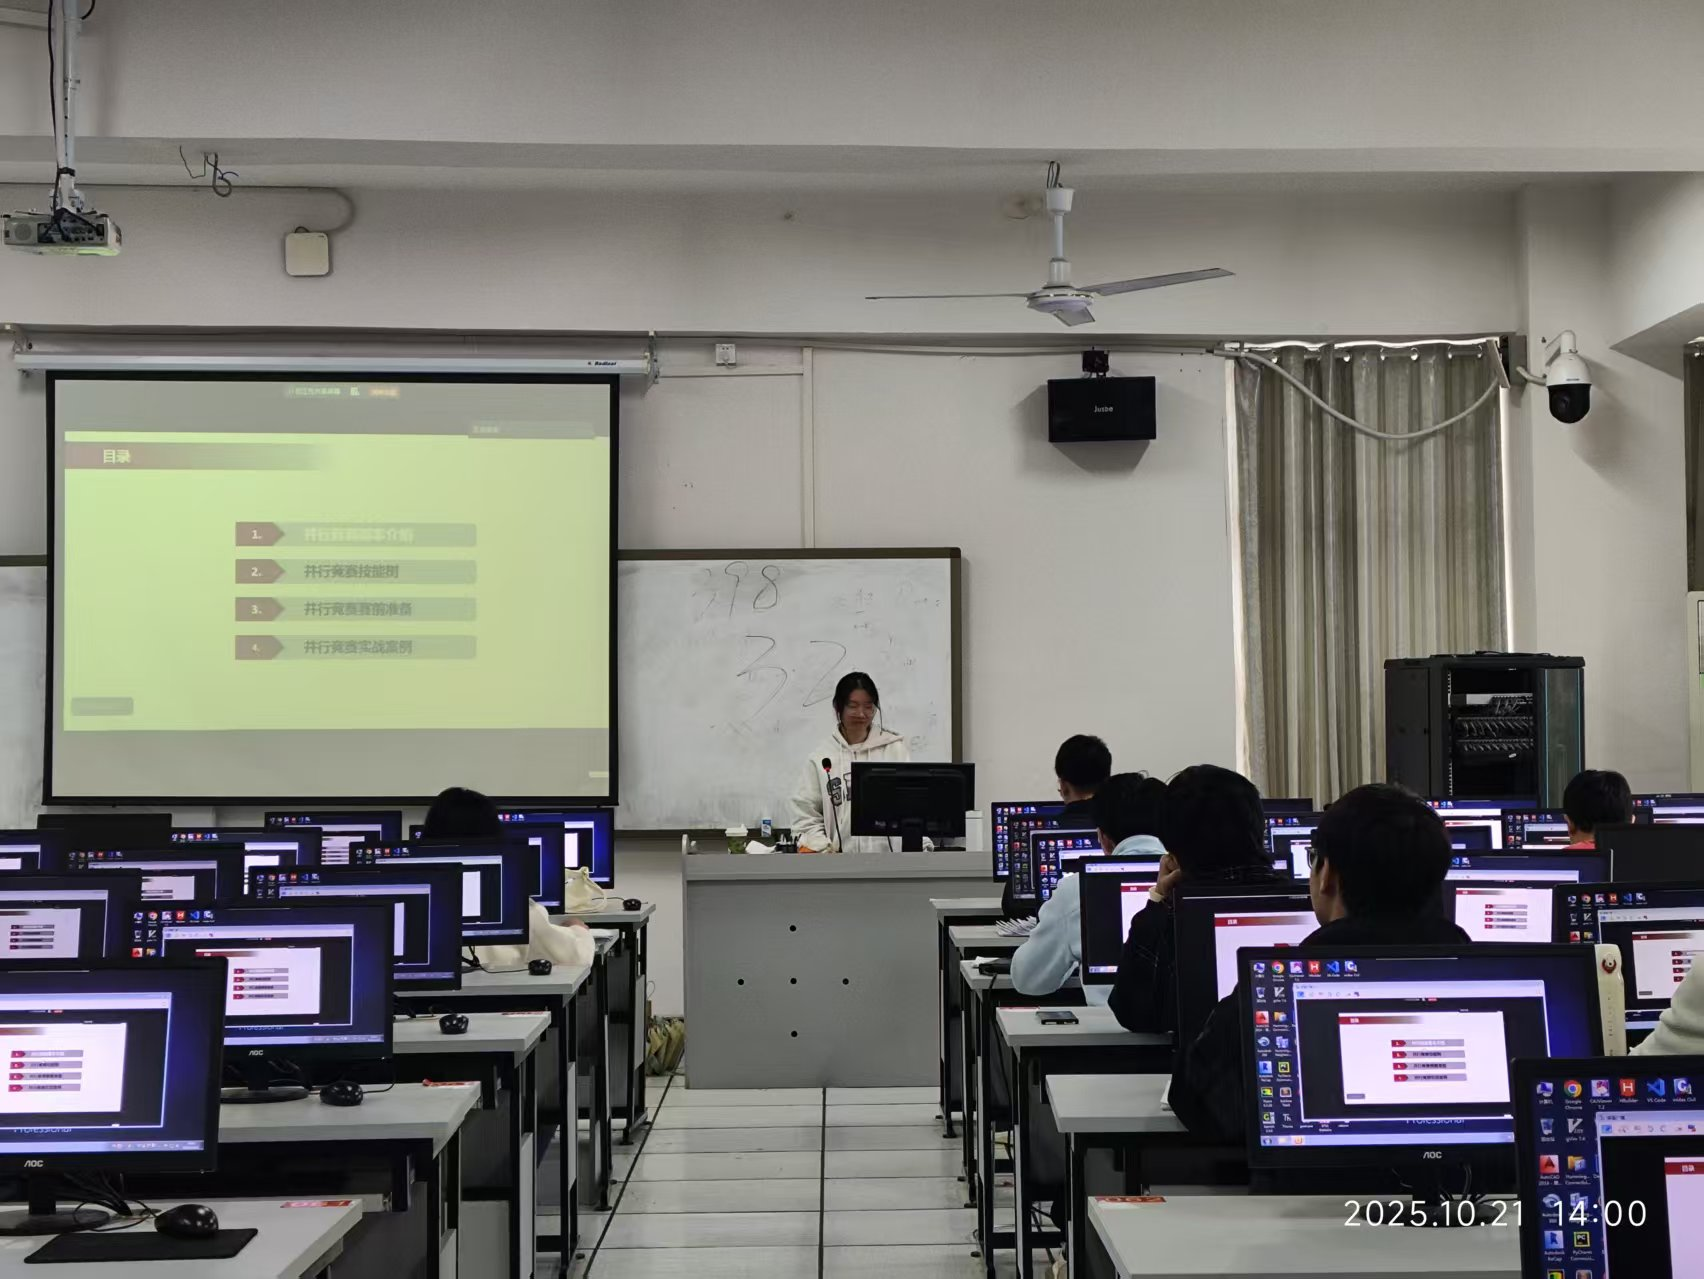
\includegraphics[width=0.48\linewidth]{figures/train0.jpg}
    } \hfill
    \subfloat{
        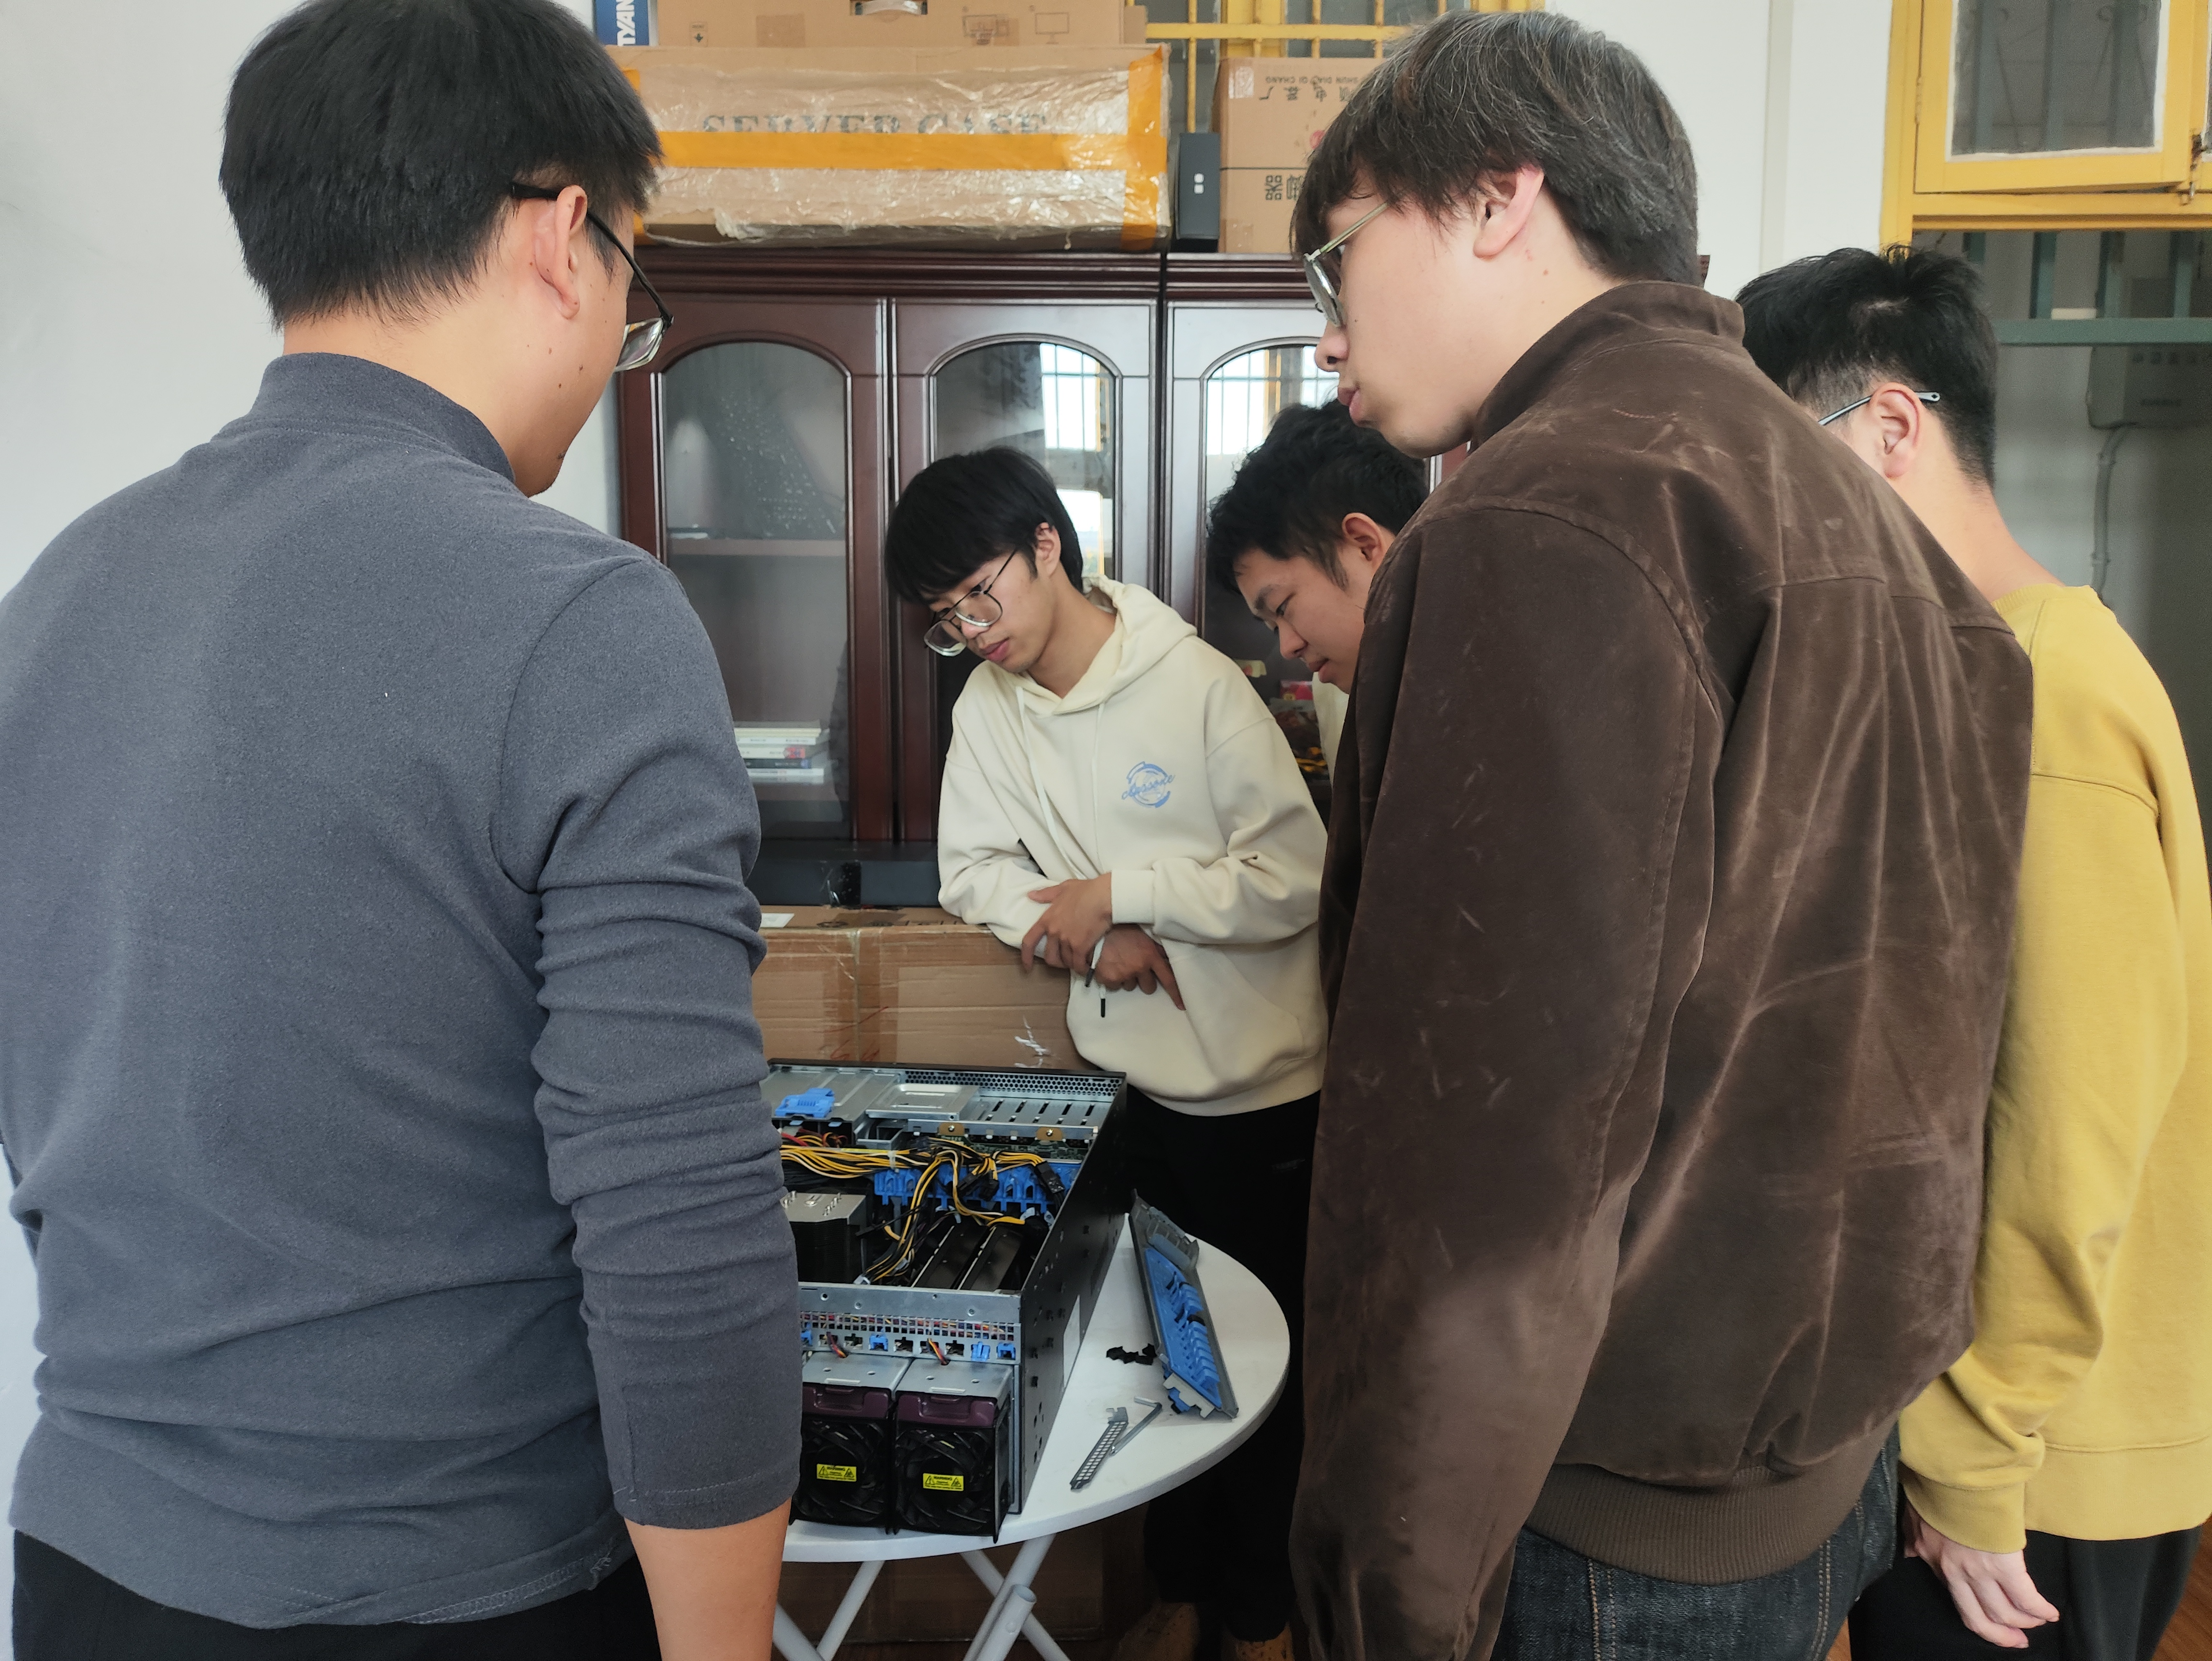
\includegraphics[width=0.48\linewidth]{figures/train1.jpg}
    } \\
    \subfloat{
        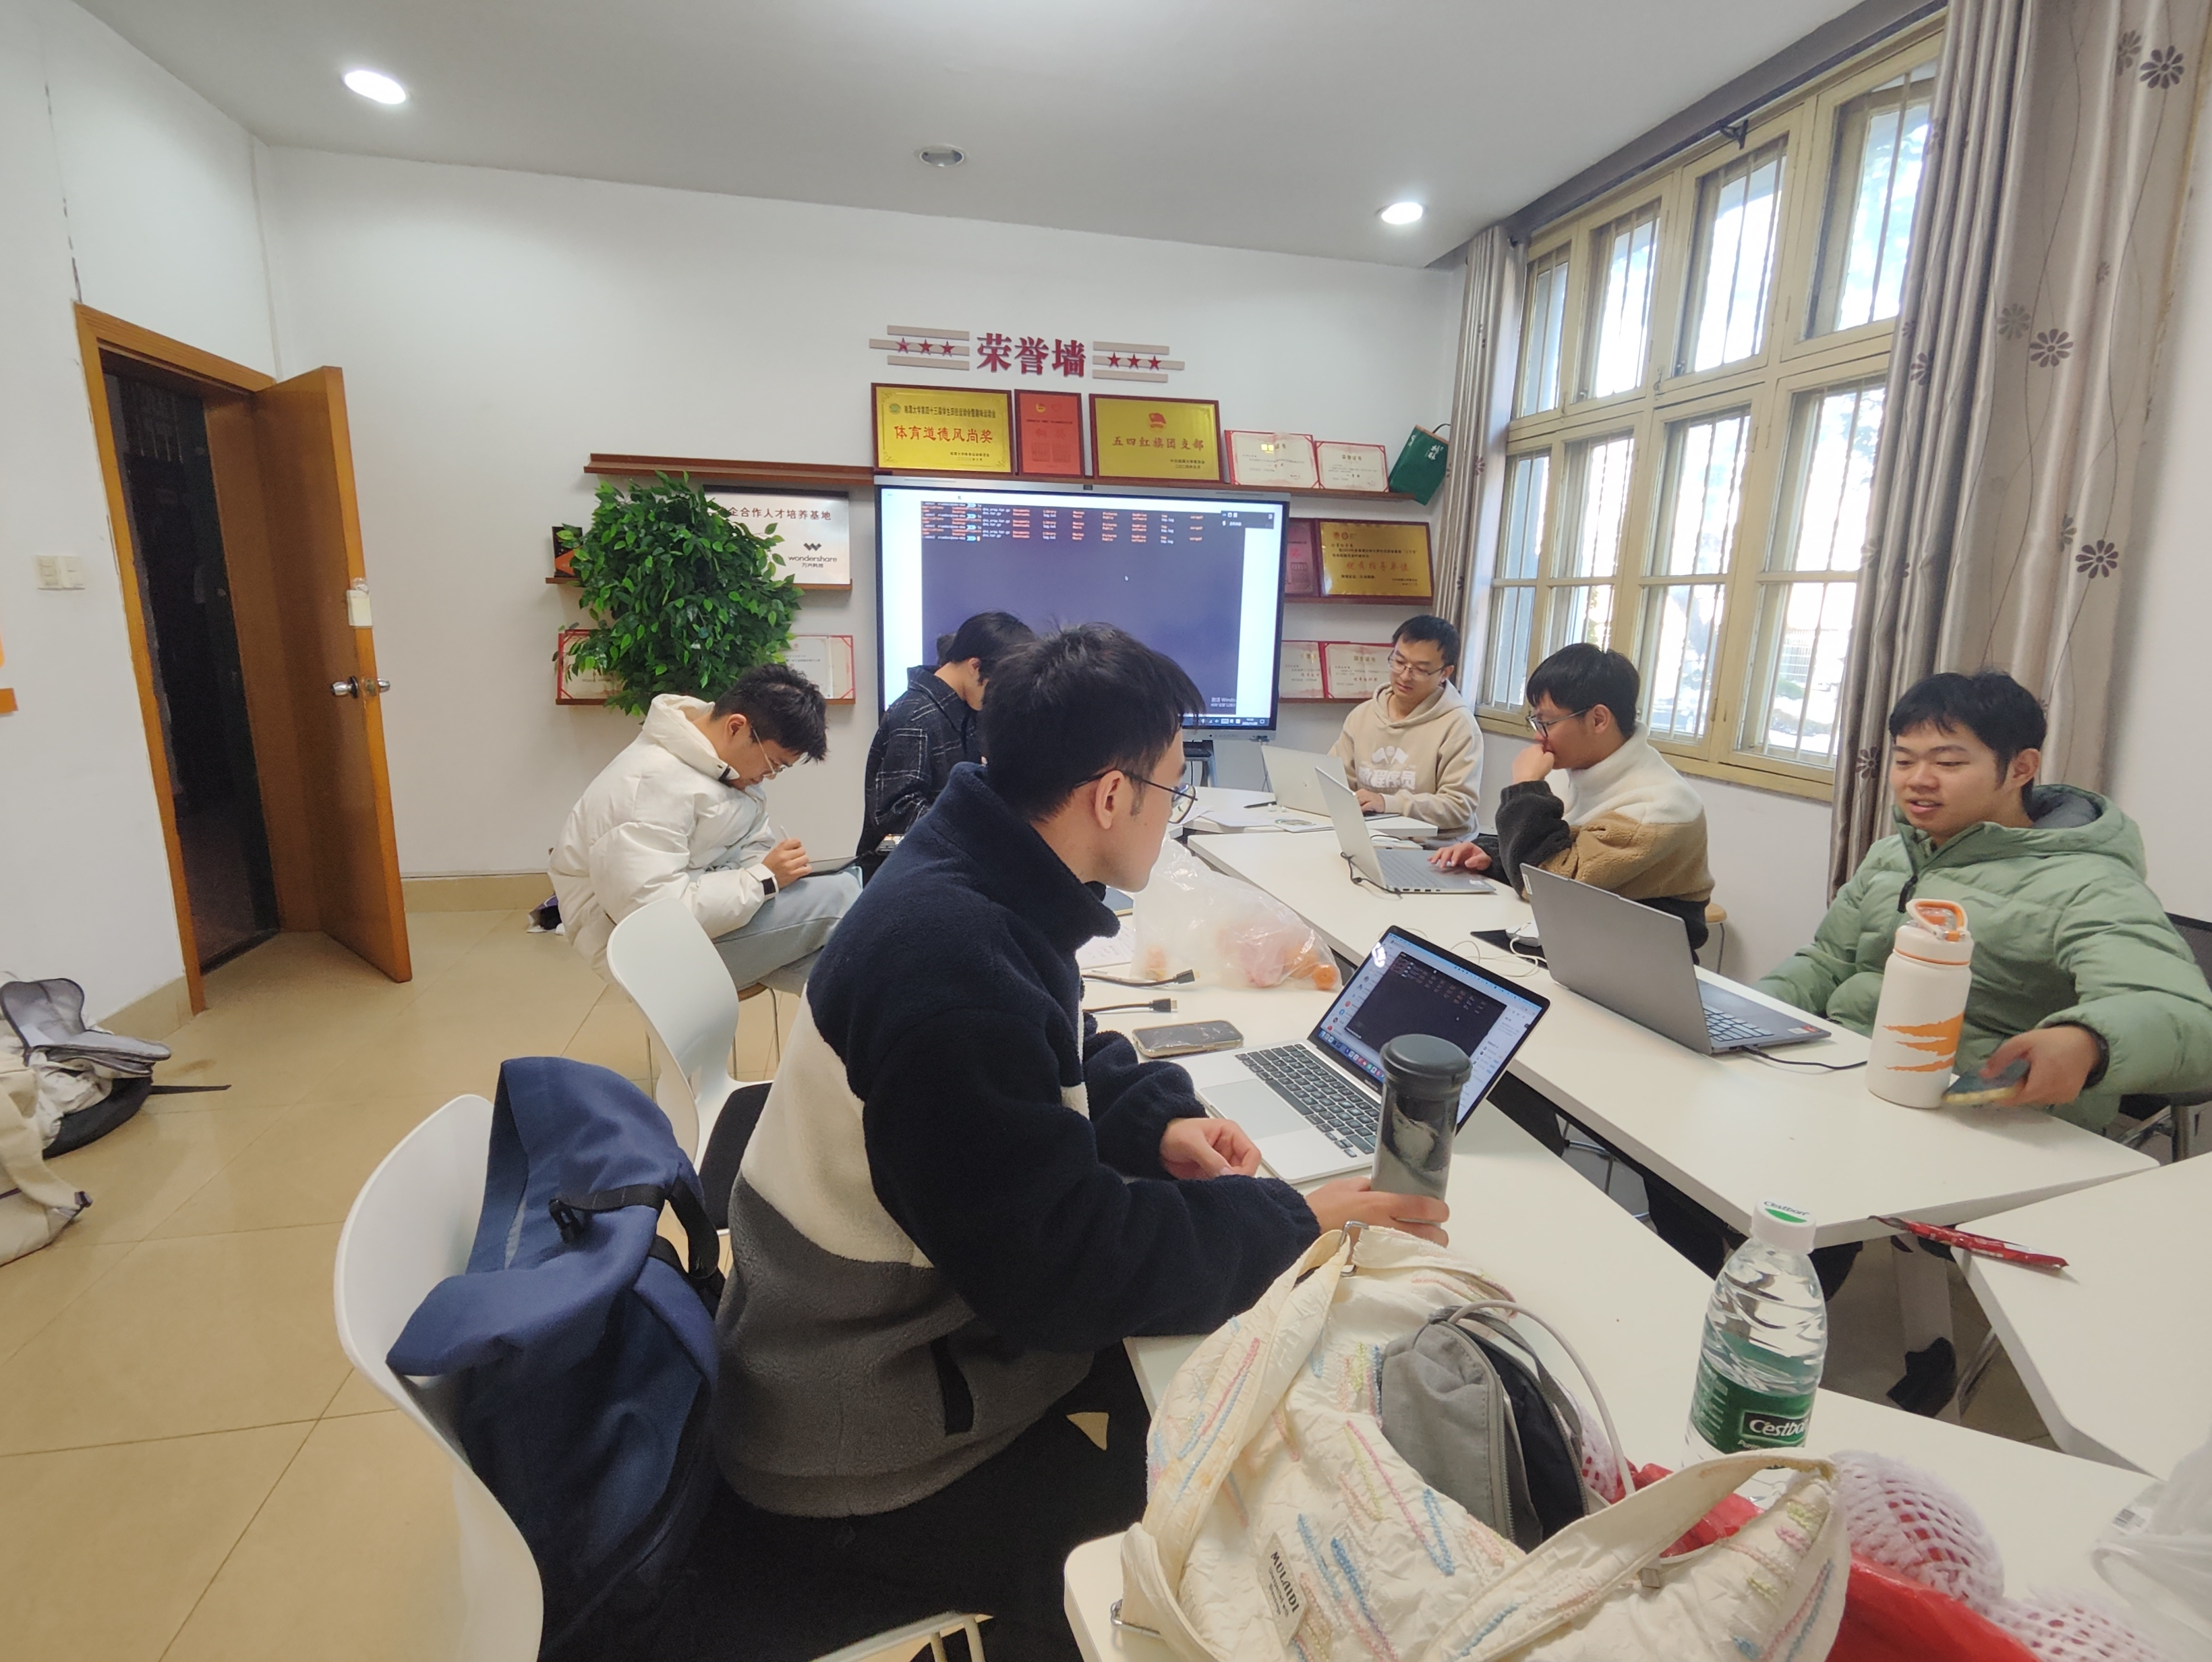
\includegraphics[width=0.48\linewidth]{figures/train2.jpg}
    } \hfill
    \subfloat{
        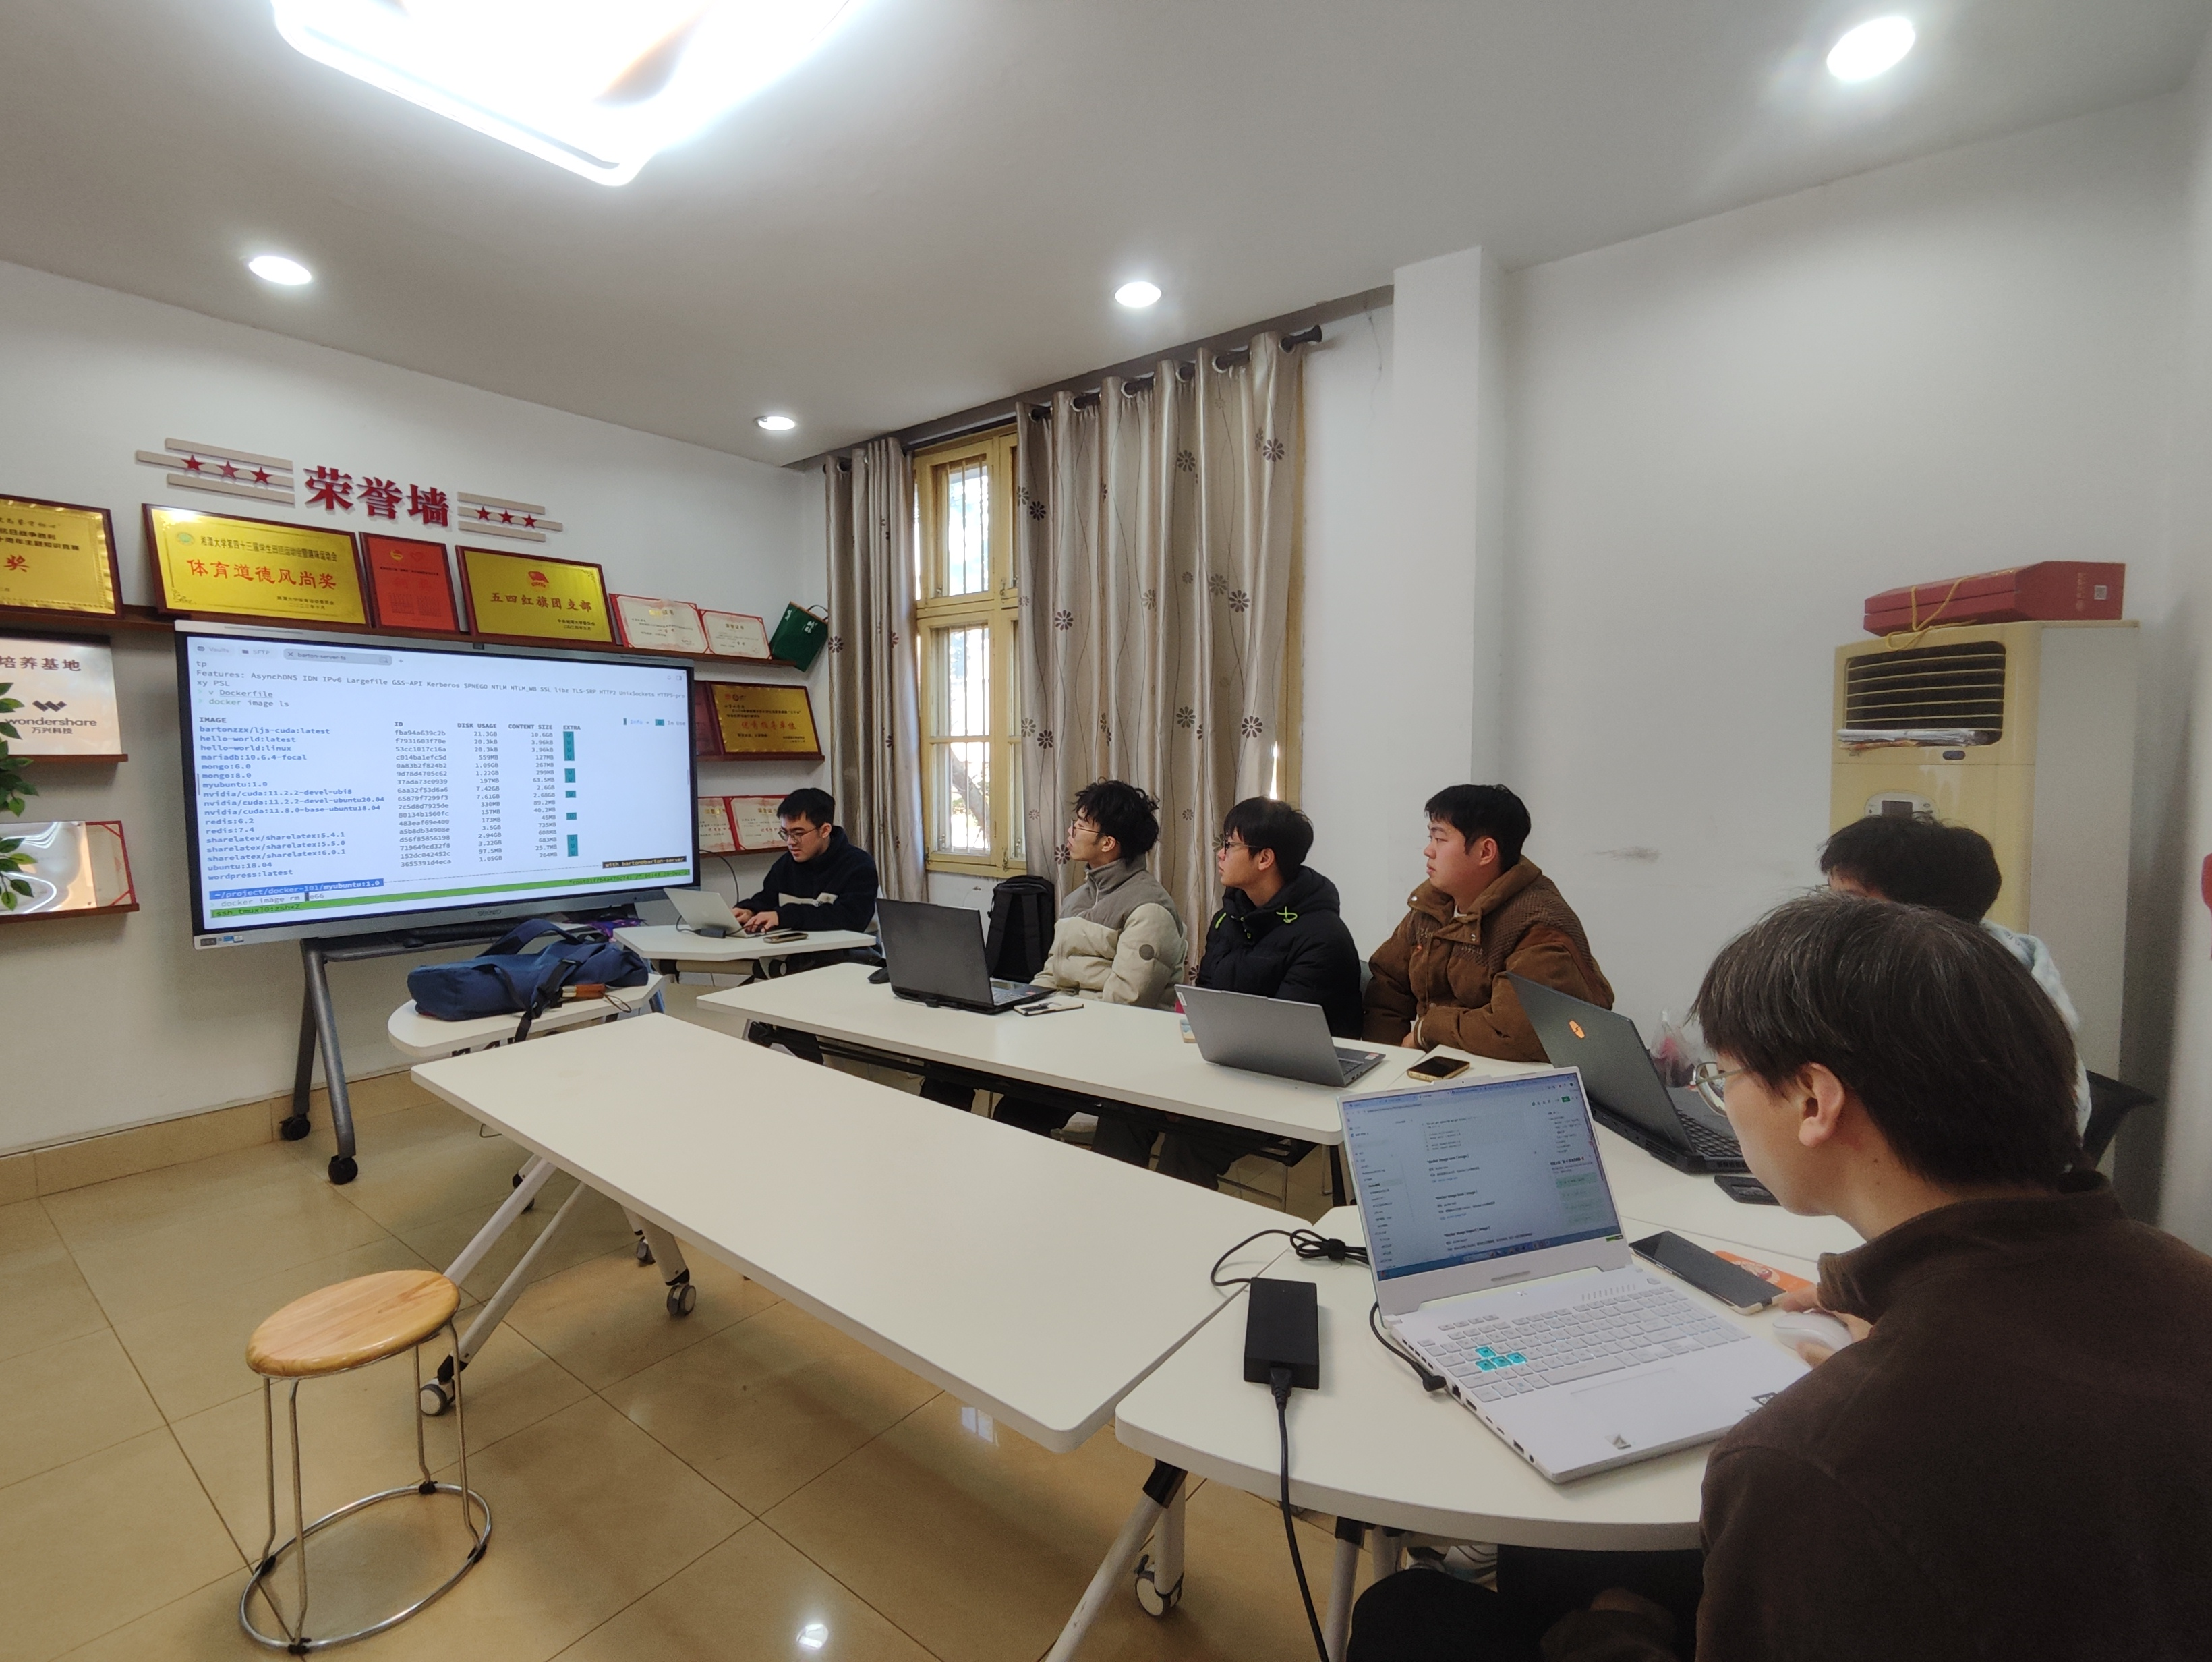
\includegraphics[width=0.48\linewidth]{figures/train3.jpg}
    } 
    \caption{Training Time}
    \label{fig:team train}
\end{figure}
% 这个比赛是由主讲并行程序设计和计算机组成原理的林培英老师发起的。林培英老师博士毕业于湖南大学，从事高性能计算研究。2024年9月开始，林老师通过课程和讲座在学校进行ASC比赛相关宣传，并制定了选拔题目。这次的比赛，从2025年9月开始，设立了新的选拔题目，然后组成了我们现在的参赛队伍。自团队成立后，林老师组织了基础知识、并行知识、优化知识等的专题培训，并多次邀请校内外前ASC参赛队员对我们进行相关经验的指导。
This competition was initiated by tutor, Peiying Lin, who teaches \textit{Parallel Programming} and \textit{Computer Organization Principles}. 
Peiying achived Ph.D. from Hunan University and is engaged in high-performance computing research. 
Starting in September 2024, Lin promoted the ASC competition through courses and lectures at the university and developed the selection criteria. 
For this year's competition, starting in September 2025, new selection criteria were established, and our current team was formed. 
Since the team's formation, Lin has organized specialized training sessions on fundamental knowledge, parallel computing, and optimization techniques, and has repeatedly invited former ASC competitors from both within and outside the university to provide guidance and share their experiences as shown in Figure \ref{fig:team train}.
% Please add the following required packages to your document preamble:
% \usepackage{subfig}



\subsection{Introduction of members}
\ 

Our participating team consists of five official members and several reserve members. 
The instructor is Peiying Lin. 
The participating students include undergraduate students majoring in Computer Science and Technology and Cyber Security. 
They are Huayu Shen, Yangkun Pei, Long Jiang, Tao Li (majoring in Computer Science and Technology, junior year) and Muyuan Chen (majoring in Cyber Security, sophomore year). 
And, the photo of our team is shown in Figure \ref{}. 
The following is an introduction of each team member.

% Please add the following required packages to your document preamble:
% \usepackage{subfig}
\begin{figure}[!htb]
    \centering
    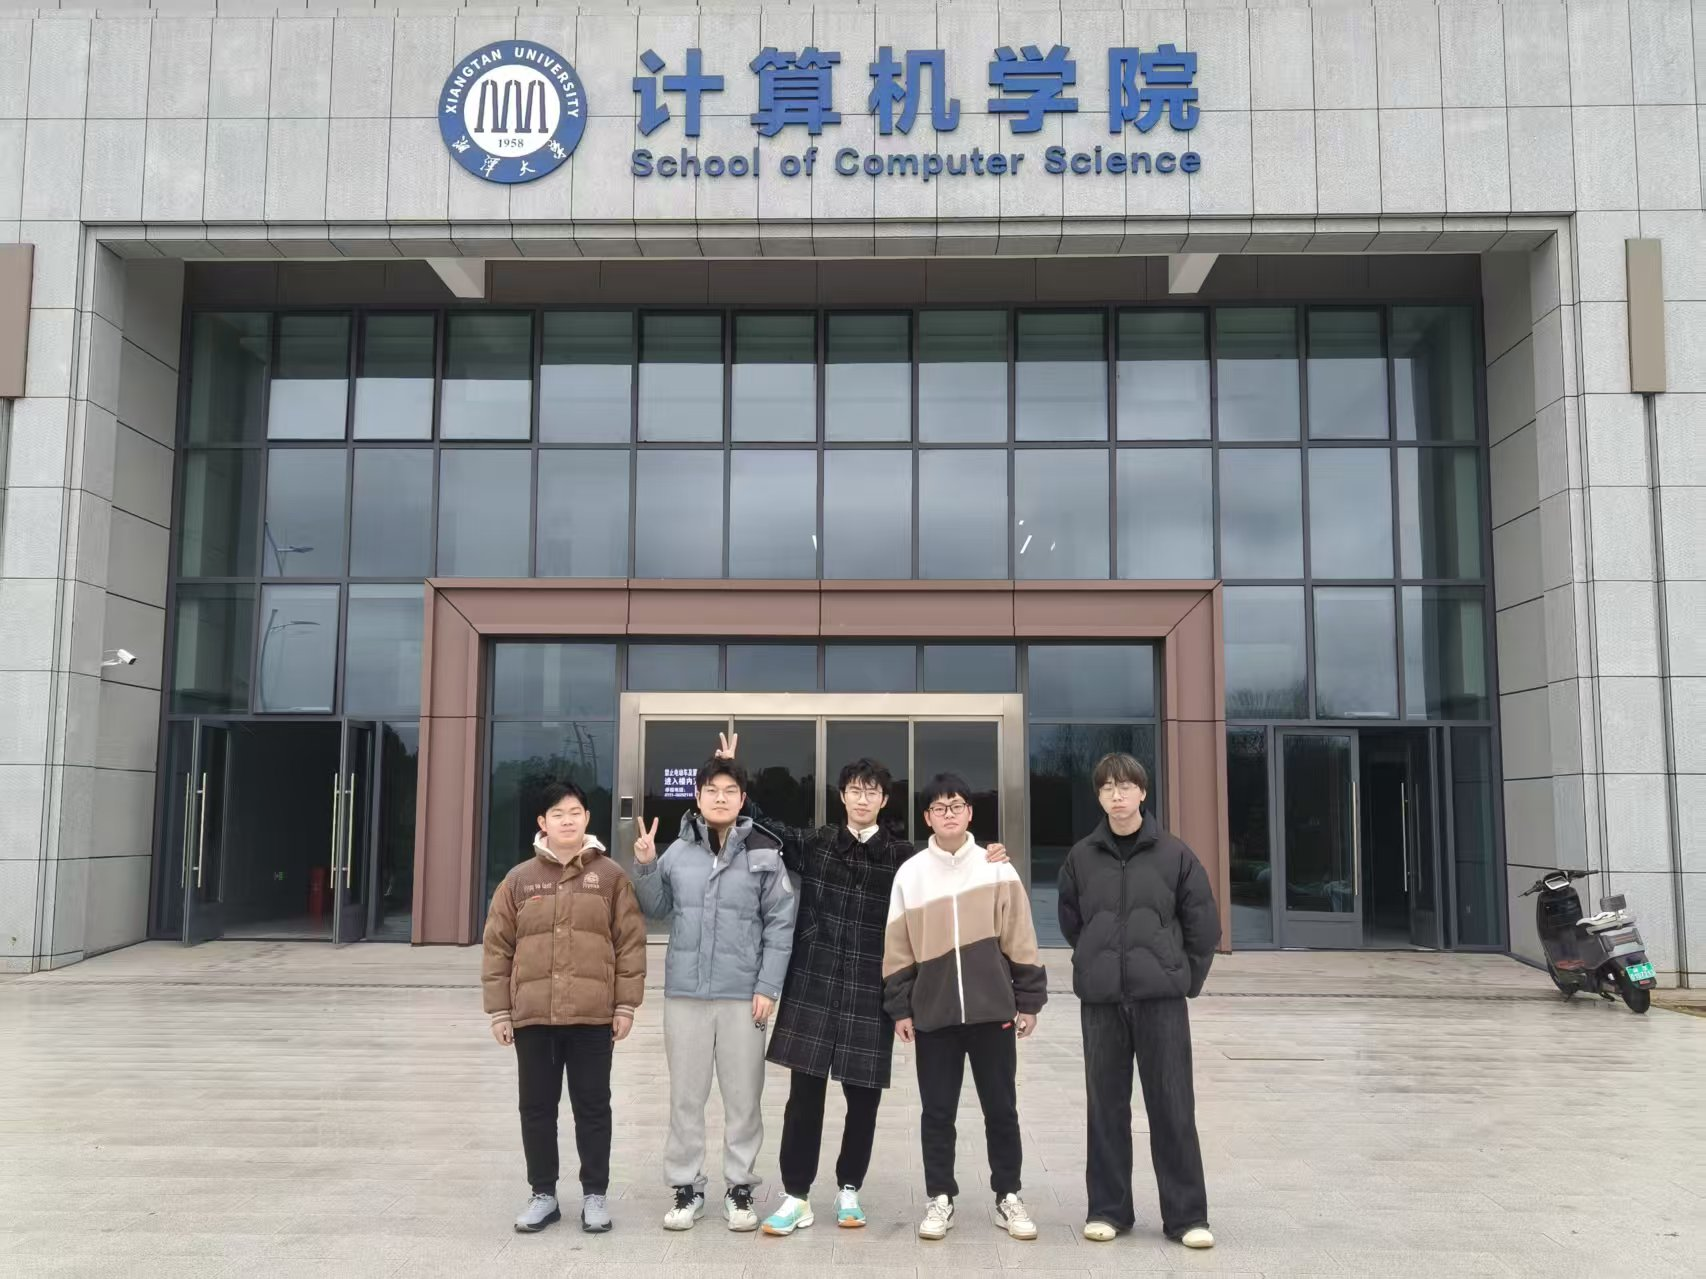
\includegraphics[width=0.7\linewidth]{figures/teammembers.jpg}
    \caption{Team Members}
    \label{fig:teams}
\end{figure}


\begin{wrapfigure}[11]{l}{0.3\textwidth} % l = 左对齐, 0.3\textwidth = 图片宽度
  \centering
  
\includegraphics[height=4cm, width=3cm]{figures/teamMeambers/huayu.jpg} 
  \label{fig:huayu}
\end{wrapfigure}
\textbf{Huayu Shen}, the team leader. 
He possesses outstanding abilities to handle difficulties, solid knowledge in computer science, and a courageous spirit of exploration. 
He is proficient in the Linux system and Git version control tools, and also skilled in MPI and OpenMP multi-threading programming. 
He once participated in the development of an online learning platform as well as an intelligent course scheduling system based on genetic algorithms and multimodal optimization.
In this ASC competition, he not only managed the overall progress but also participated in the optimization of HPL tests and the performance optimization of AMSS-NCKU. 
% \vspace{1em} % 间距

\begin{wrapfigure}[10]{l}{0.3\textwidth} % l = 左对齐, 0.3\textwidth = 图片宽度
  \centering
  
\includegraphics[height=4cm, width=3cm]{figures/teamMeambers/yangkun.jpg} 
  \label{fig:yangkun}
\end{wrapfigure}
\textbf{Yangkun Pei} is good at C/C++, Python and Shell scripting for cross-platform development, familiar with MPI, OpenMP and CUDA GPU acceleration technologies.
He possesses the ability to design and optimize multi-level parallelization algorithms. 
He is also familiar with the Linux development environment, CMake build toolchain and advanced optimization options of GCC/Intel compilers. 
In this competition, he is responsible for the deployment and operation of AMSS-NCKU and the design and implementation of its optimization plan. Additionally, he also completed the performance optimization analysis of HPCG on the CPU.
% \vspace{1em} % 间距


\begin{wrapfigure}[12]{l}{0.3\textwidth} % l = 左对齐, 0.3\textwidth = 图片宽度
  \centering
  
\includegraphics[height=4cm, width=3cm]{figures/teamMeambers/jianglong.jpg} 
  \label{fig:jianglong}
\end{wrapfigure}

\textbf{Long Jiang}  is skilled in mainstream programming languages, and has strong abilities in algorithm design and analysis. 
He has a deep understanding of MPI and OpenMP parallel programming models, and has a preliminary understanding of the CUDA C programming model. 
He is familiar with the Linux operating system and is proficient in using various Linux commands and uses WSL2 as his daily development platform.
He is also familiar with machine learning algorithm. 
In this competition, he takes charge of the UnifoLM-WMA-0 optimization, employing various optimization methods to achieve acceleration, such as I/O optimization, cache optimization, and operator optimization, etc. 
In addition, he was also responsible for the CPU test optimization of HPCG.


\begin{wrapfigure}[9]{l}{0.3\textwidth} % l = 左对齐, 0.3\textwidth = 图片宽度
  \centering
  
\includegraphics[height=4cm, width=3cm]{figures/teamMeambers/muyuan.jpg} 
  \label{fig:muyuan}
\end{wrapfigure}
\textbf{Muyuan Chen} has a passion for computers and possesses strong learning abilities. 
He is proficient in using Linux and Git, and is well-versed in C/C++ and Java programming languages. 
He has a strong ability in algorithm design and implementation, and can quickly adapt to different programming environments. 
He is familiar with technologies such as model inference security and security protection. 
In this competition, he mainly took charge of the HPCG GPU optimization part and the analysis and design of the UnifoLM-WMA-0 optimization.


\begin{wrapfigure}[7]{l}{0.3\textwidth} % l = 左对齐, 0.3\textwidth = 图片宽度
  \centering
  
\includegraphics[height=4cm, width=3cm]{figures/teamMeambers/liTao.jpg} 
  \label{fig:liTao}
\end{wrapfigure}

\textbf{Tao Li} has a solid foundation in computer science and a strong spirit of exploration. 
He is proficient in Linux and Git, skilled in C and C++ programming, familiar with MPI and OpenMP parallel programming, and has a certain foundation in AI. 
In this competition, he mainly took charge of the design and analysis of the HPC system, and participated in the analysis and design of UnifoLM-WMA-0.

\vspace{4em}



% % 我们的参赛队伍由五名正式成员和多名后备成员组成，指导老师为林培英。参赛学生包括计算机科学与技术和网络空间安全专业的本科生，他们分别是沈华宇、裴杨坤、江龙、李涛(计算机科学与技术专业，大三)和陈牧远(网络空间安全专业，大二)。以下是每位队员的详细介绍。



% % 沈华宇，队长。他具备卓越的面对困难的能力、扎实的计算机科学功底以及勇于挑战的探索精神。熟练掌握 Linux 系统和 Git 版本控制工具，熟练掌握MPI 和 OpenMP 多线程编程以。曾在“蓝桥杯” Java 组获得省奖，参与开发过一个较为完善的在线学习平台以及基于遗传算法以及多模态优化的智能排课系统。在此次 ASC 竞赛中，作为队长，他不仅负责整体进度管理，还参与 AMSS-NCKU 的性能优化，通过并行计算以及内存管理提高了算法效率和速度。




% % 裴杨坤，掌握C/C++、Python 及 Shell 脚本跨平台开发，熟悉MPI、OpenMP 与 CUDA GPU 加速技术，具备多层级并行化算法设计与调优能力；熟悉 Linux 开发环境、CMake 编译工具链及 GCC/Intel 编译器高级优化选项。在本次比赛中，他负责AMSS-NCKU的部署运行及其优化方案的设计与实现。此外，他还完成了HPCG在CPU中的性能优化分析。



% %江龙，熟练掌握 C，C++，Java 和 pyhton 高级编程语言，拥有较强的算法设计与分析能力，能够快速适应不同的编程环境。深入掌握 MPI 和 OpenMP 并行编程模型，对 CUDA C 编程模型有着初步的理解，具有大规模并行计算和多线程编程的能力。熟悉 Linux 操作系统，熟练使用各类 Linux 命令，以 wsl2 作为日常开发平台，能够进行有效的模型部署和准确的测试结果。对传统算法具有较为扎实的基础，熟悉机器学习算法思想，具备人工智能（AI）基础。在本次比赛中主要负责 Embodied World Model Optimization部分，尝试采用 IO 优化、DeepCache 利用时序冗余的面训练策略，FlashAttention-2 优化和内核融合等方式加快 unifolm-wma 在 inference 时的速度。


% % 李涛，计算机基础扎实，富有探索精神。他熟练掌握Linux和Git，精通C和C++编程，并熟悉MPI和OpenMP并行编程，且具备一定人工智能（AI）基础。在此次比赛中，他主要负责HPC系统的设计与分析，并参与UnifoLM-WMA-0的分析与设计。

% % 陈牧远，热爱计算机，学习能力强。他熟练使用Linux和Git，精通C/C++和Java编程语言，具备强大的算法设计与实现能力，能够迅速适应不同的编程环境。熟悉模型推理安全，安全防护等技术。在这次比赛中，他主要负责HPCG GPU 优化部分和UnifoLM-WMA-0优化方案分析与设计。


\subsection{Team slogan}
\ 

\textbf{Code Flows, Nodes Ignite, Victory Follows.}

\clearpage
% \textbf{Unlimited Algorithms, Fearless Supercomputing, Victory Walks with Us}%5页
\newpage
%important---今年：突出了AI；点明了必须要有的部分；不超过15页。
\section{Design of our HPC System}
This section introduces the design of the AI and HPC cluster system.
It begins with an overview of the HPC system architecture, followed by detailed discussions of hardware configuration, software configuration and the interconnection architecture.
Then, we do a comprehensive performance analysis for the computing performance and power consumption.

\subsection{Architectural Diagram Overview}%c-1
\

The HPC cluster design we proposed is shown in Figure \ref{fig:HPCDesign}.
This system adopts a dual-network design with management and data separated, consisting of 4 heterogeneous computing nodes. 
It not only meets the requirements of the competition benchmark but also ensures the high availability of the system. 
\begin{enumerate}
    \item \textbf{Access and Out-of-Band Management: }External users connect to the gigabit Ethernet switch via workstations and utilize the IPMI 2.0 protocol (the blue solid line in the figure) to achieve bottom-level monitoring and out-of-band management of the entire cluster hardware. 
    It supports remote scheduling, power on/off operations, and sensor status monitoring. 
    \item \textbf{Cluster scheduling logic:} Node 0 is configured as the master node (``Master Node"), and cluster management is achieved through a gigabit CAT6 link (indicated by the dotted line in the figure). 
    Its core functions include job scheduling, task distribution, compilation environment hosting, and maintenance of the NFS shared file system. 
    \item \textbf{High-speed interconnection architecture:} The system computing network adopts NDR InfiniBand interconnection (the black solid lines in the figure), and each node is connected to the NDR-IB switch through high-performance HCA cards, providing extremely high throughput bandwidth and microsecond-level latency. 
    \item \textbf{Heterogeneous computing unit}: Each node is constructed based on a dual-processor server and is connected via the PCIe bus to two AMD Radeon Pro W7900D graphics cards. 
    The entire cluster is equipped with a total of 8 high-performance GPUs. 
    With outstanding single/double precision floating-point computing capabilities, it precisely meets the requirements of complex HPC simulations and large-scale AI application.
\end{enumerate}




% Please add the following required packages to your document preamble:
% \usepackage{subfig}
\begin{figure}[!htb]
    \centering
    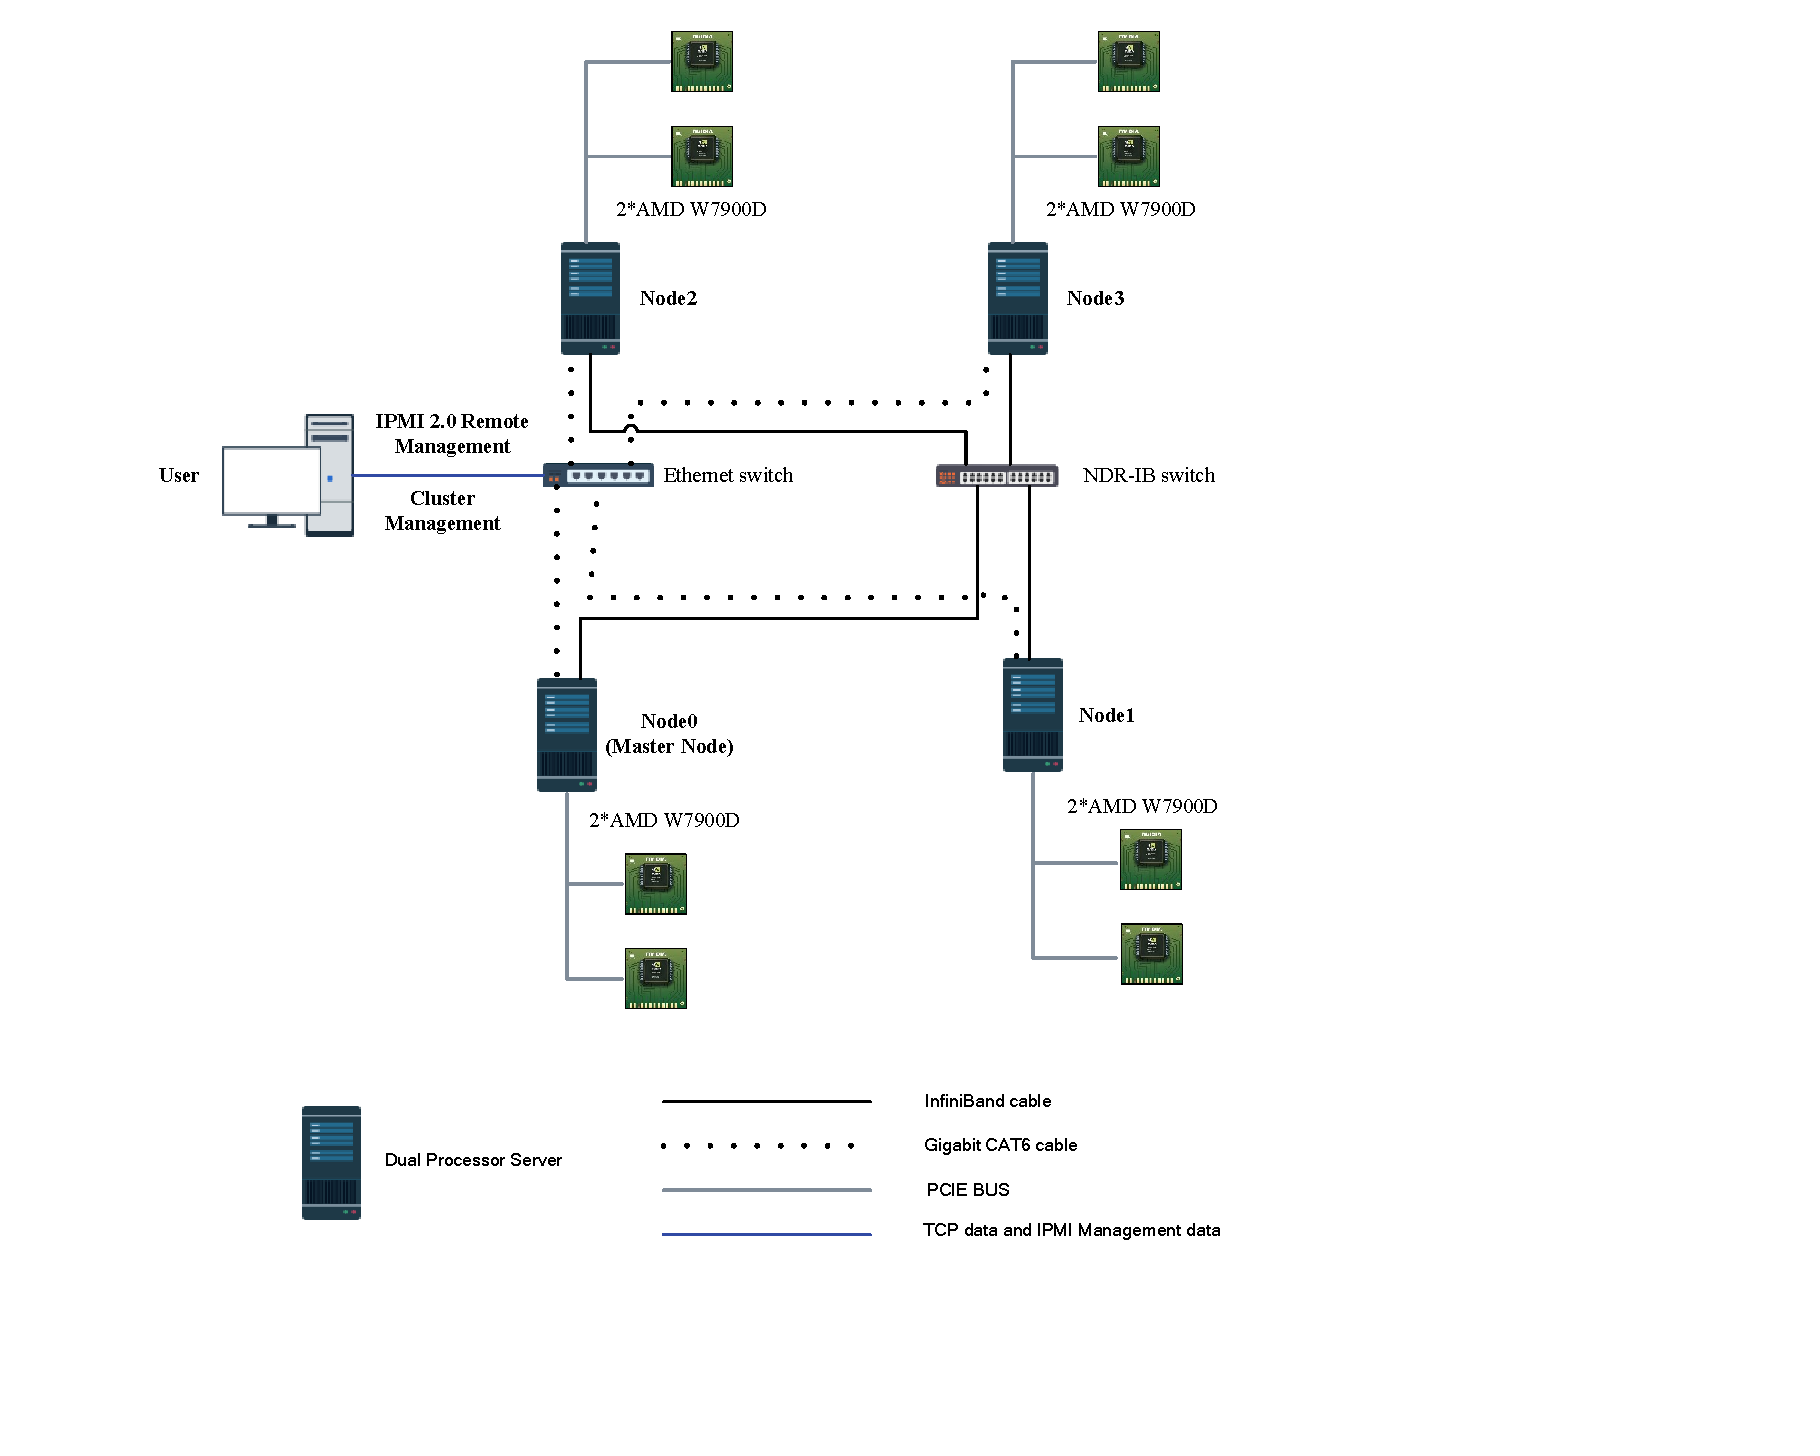
\includegraphics[width=0.98\linewidth]{figures/hpcDesign-0221.pdf}
    \caption{Architectural Diagram Overview}
    \label{fig:HPCDesign}
\end{figure}


\subsection{System Configuration and Architecture Analysis}%b
\


\subsubsection{Hardware Configurations}
\


The complete technical specifications of the designed HPC system are systematically presented in Table \ref{tab:hpc hardware}.
This high-performance computing system is a small heterogeneous computing cluster, which is a cost-effective and balanced heterogeneous workstation cluster. 
Although its local storage I/O speed is slightly conservative, its powerful interconnection capability and computing density enable it to fully handle the ASC supercomputing competition and complex AI research tasks. 
The detailed analysis is as follows. 
Firstly, in terms of CPU processors, each computing node is equipped with two processors recommended by the committee, namely AMD EPYC 9755 with the latest Zen 5 architecture, each with 128 cores and 512M cache. 
The entire cluster has a total of 1024 physical cores, and it has strong capabilities in multi-threaded tasks and instruction-level parallelism (ILP). 
Secondly, at the accelerator (GPU) level, the entire cluster is equipped with 8 AMD Radeon Pro W7900D workstation graphics cards, with 2 cards per node. 
The W7900D is based on the RDNA 3 architecture, with a huge memory capacity and high bandwidth, making it a powerful tool for AI inference and graphics rendering.
In the storage and memory level, each node is configured with 768GB DDR5 memory ($32GB \times 24$), with a clock speed of up to 6400 MT/s, ensuring a large bandwidth to meet the data feeding requirements of a multi-core CPU. 
The system disk uses a 960GB SATA SSD, balancing startup speed and stability. 
Finally, the high-speed network uses the NVIDIA Quantum-2 NDR InfiniBand switch, providing a single port throughput of 400Gbps, and combined with the MCX75310AAS-NEAT HCA card, it achieves extremely low one-way latency.

\begin{table}[h]
\centering
\caption{Hardware resources details}
\label{tab:hpc hardware}
\renewcommand{\arraystretch}{1.2} % 增加行间距，使表格更美观
\begin{tabular}{|c|l|c|}
\hline
\rowcolor{myyellow}
\textbf{Item} & \multicolumn{1}{c|}{\textbf{Name}} & \textbf{Quantity} \\ \hline
 & CPU: AMD 9755-EPYC 2.7\_128C\_512M * 2 & 4 \\ \cline{2-3} 
 & Memory: 32GB * 24, DDR5, 6400 MT/s & 4 \\ \cline{2-3} 
 & Hard disk: 960GB SSD SATA * 1 & 4 \\ \cline{2-3} 
\multirow{-4}{*}{Dual Processor Server} & Motherboard Power Consumption & 4 \\ \hline
GPU & AMD W7900D & 8 \\ \hline
HCA & NDR400: NVIDIA MCX75310AAS-NEAT & 4 \\ \hline
 & Ethernet switch: 10/100/1000 MB/s, 24 ports Ethernet switch & 1 \\ \cline{2-3} 
\multirow{-2}{*}{Switch} & \begin{tabular}[c]{@{}l@{}}NDR-IB switch: NVIDIA Quantum (TM)-2 NDR InfiniBand Switch\\ , 64-ports NDR, 32 OSFP ports, unmanaged, P2C airflow (forward)\end{tabular} & 1 \\ \hline
 & Gigabit CAT6 cables & 5 \\ \cline{2-3} 
\multirow{-2}{*}{Cable} & InfiniBand cable & 4 \\ \hline
\end{tabular}
\end{table}

\subsubsection{Software Configurations}
\

Since the CPU and GPU of this HPC system are both sourced from AMD, in order to enable the system to run large-scale computing and artificial intelligence operations efficiently, its main software configuration follows the AMD recommended configuration\footnote{https://www.amd.com/en/developer.html}. 
The details are shown in Table \ref{tab:hpc software}. 
The operating system selected is Ubuntu 24.04 LTS as the underlying operating system. 
As the latest long-term support version, it can provide excellent stability and compatibility for high-performance hardware. 
For GPU heterogeneous computing, the latest stable version ROCm 7.2 is configured, providing complete support from the underlying driver to the high-level library, including MIOpen (deep learning primitive library) and rocBLAS (linear algebra library). 
For the CPU system deployment, Zen Software Studio 2.0 is configured, whose core includes AOCC (a compiler highly optimized for the Zen 5 architecture), AOCL (an optimized math library), ZenDNN (an inference acceleration library), and AMD uProf (a performance analysis tool). 
At the application layer, Anaconda is used to build an isolated and repeatable scientific computing environment, with the latest versions of PyTorch, TensorFlow, and JAX, etc. integrated.



\begin{table}[h]
\centering
\caption{Software resources details}
\label{tab:hpc software}
\renewcommand{\arraystretch}{1.2} % 增加行间距，使表格更美观
\begin{tabular}{|C{4cm}|L{10cm}|C{2cm}|}
\hline
\rowcolor{myyellow}
\textbf{Item} & \textbf{Name} & \textbf{Version} \\ \hline
Application software & Anaconda(including PyTorch, TensorFlow, JAX and so on) & Version 2.3 \\ \hline
GPU & ROCm  & Version 7.2 \\ \hline
CPU & AMD Zen Software Studio(including AMD uProf, AOCL, AOCC, ZenDNN and so on) & Version 2.0 \\ \hline
Operating system & Ubuntu & 24.04 LTS \\ \hline
\end{tabular}
\end{table}



\subsubsection{Interconnection Architecture}
\

As shown in the Figure \ref{fig:HPCDesign}, the HPC system of this design adopts a ``management network + data network" separated architecture and uses a star topology. 
The ``Master Node" serves as the cluster entry point and is mainly responsible for task distribution management. 
The compute nodes are mainly responsible for computing. 
Low-latency data exchange is achieved through InfiniBand, and remote IPMI and cluster control are realized through Ethernet.

\subsection{Computing Performance Description}
\

Based on the relevant parameters of AMD 9755-EPYC \footnote{https://www.amd.com/en/products/processors/server/epyc/9005-series/amd-epyc-9755.html}
and AMD Radeon Pro W7900D\footnote{https://www.amd.com/en/products/graphics/workstations/radeon-pro/w7900.html}, the performance analysis of the CPU and GPU for our HPC system is as follows.

The peak performance calculation formula for the CPU is 
\begin{equation}
         \text{Peak Performance} = \text{Clock Speed} \times \text{Cores} \times \text{Operations per Cycle}.
\end{equation}

\begin{enumerate}
    \item \textbf{Clock speed: }Since the ``Base clock" of AMD 9755-EPYC is 2.7GHz and the ``Max. Boost Clock" is 4.1GHz, here we will calculate its highest computing performance. 
    Therefore, we set the clock speed to 4.1GHz.
    \item \textbf{Cores: }HPC consists of 4 computing nodes, and each computing node contains 2 CPUs with 128 cores. 
    Therefore, the cores included in HPC are $4{\times}2{\times}128{=}1024$.
    \item \textbf{Operations per Cycle: }In the competition, if floating-point operations use single-precision floating-point numbers, then since the Zen 5 architecture has a complete 512-bit (512-bit) vector unit, each 512-bit register can store 8 FP64 numbers. 
    Also, since the CPU supports FMA (Fused Multiply-Add) instructions (2 FMA units), one cycle can complete one multiplication and one addition (counted as 2 operations). 
    Therefore, the single-cycle operation count of AMD 9755-EPYC can be $2{\times}8{\times}2{=}32 flops/Cycle$.
\end{enumerate}  

Based on the above information, the final peak CPU performance of the HPC is
\begin{equation}
         4.1GHz{\times}1024(Cores){\times}32 (\text{Operations per Cycle})\\
          =134.3488TLOPs
\end{equation}


According to the official website information, the peak double float precision(FP64), single float precision (FP32 Vector)  and half float precision(FP16) performance of the AMD Radeon Pro W7900D single GPU are 1.916 Tflops, 61.3 Tflops and 123 Tflops, respectively.
And there are a total of 8 GPUs in the cluster. 
Therefore, the overall theoretical peak performance of the GPUs is based on different precisions are as follows.
\begin{equation}
    \text{FP64 Peak Performance} {=} 1.916 TLOPs \times 8 {=} 15.328 TLOPs.
\end{equation}

\begin{equation}
    \text{FP32 Peak Performance} {=} 61.3 TLOPs \times 8 {=} 490.4 TLOPs.
\end{equation}

\begin{equation}
    \text{FP16 Peak Performance} {=} 123 TLOPs \times 8 {=} 984 TLOPs.
\end{equation}



\subsection{Power Consumption Description}%c-2
\


Our HPC cluster comprises four computing nodes. 
This section provides a detailed analysis of power consumption patterns for both GPU and CPU operations at individual node level and cluster-wide scale, as detailed in Table \ref{tab:power}. 
As can be seen from the table, for a single node, the CPU computing power consumption is $1054W{+}40W{=}1094W$, and the GPU computing power consumption is $354W{+}2×295W{=}944W$, both of which meet the power consumption requirement of less than $2000W$. 
For the entire cluster, the CPU computing power consumption is
$4926W$, and the GPU computing power consumption is $4326W$, which also meet the power consumption requirement of less than $5000W$.




\begin{table}[htbp]
\centering
\small
\caption{Power Consumption Details}
\label{tab:power}
\begin{tabular}{|C{1.8cm}|C{2.5cm}|L{7.5cm}|C{1.8cm}|}
\hline
\rowcolor{myyellow}
\textbf{Mode} & \textbf{Name} & \multicolumn{2}{|c|}{\arraybackslash\textbf{Power Consumption}} \tabularnewline
\hline
\multirow{11}{=}{CPU computing} 
 & \multirow{4}{=}{Dual Processor Server} 
   & CPU: AMD 9755-EPYC2.7 128C 512M * 2 (450w * 2) 
   & \multirow{4}{*}{1054w*4} \tabularnewline
\cline{3-3}
 &  & Memory: 32GB * 24, DDR5, 6400 MT/s (5w * 24) &  \tabularnewline
\cline{3-3}
 &  & Hard disk: 960GB SSD SATA * 1 (4w * 1) &  \tabularnewline
\cline{3-3}
 &  & Motherboard Power Consumption (30w) &  \tabularnewline
\cline{2-4}
 & GPU & AMD W7900D & 20w*8 \tabularnewline
\cline{2-4}
 & HCA & NDR400: NVIDIA MCX75310AAS-NEAT & 30w*4 \tabularnewline
\cline{2-4}
 & \multirow{2}{*}{Switch} 
   & Ethernet switch: 10/100/1000 MB/s, 24 ports Ethernet switch 
   & 30w \tabularnewline
\cline{3-4}
 &  & NDR-IB switch: NVIDIA Quantum (TM)-2 NDR InfiniBand Switch, 64-ports 
   & 400w \tabularnewline
\cline{2-4}
 & \multicolumn{2}{c|}{\textbf{Total}} & \textbf{4926w} \tabularnewline
\hline
\multirow{11}{=}{GPU computing} 
 & \multirow{4}{=}{Dual Processor Server} 
   & CPU: AMD 9755-EPYC2.7 128C 512M * 2 (100w * 2) 
   & \multirow{4}{*}{354w*4} \tabularnewline
\cline{3-3}
 &  & Memory: 32GB * 24, DDR5, 6400 MT/s (5w * 24) &  \tabularnewline
\cline{3-3}
 &  & Hard disk: 960GB SSD SATA * 1 (4w * 1) &  \tabularnewline
\cline{3-3}
 &  & Motherboard Power Consumption (30w) &  \tabularnewline
\cline{2-4}
 & GPU & AMD W7900D (295w) & 295w*8 \tabularnewline
\cline{2-4}
 & HCA & NDR400: NVIDIA MCX75310AAS-NEAT & 30w*4 \tabularnewline
\cline{2-4}
 & \multirow{2}{*}{Switch} 
   & Ethernet switch: 10/100/1000 MB/s, 24 ports Ethernet switch 
   & 30w \tabularnewline
\cline{3-4}
 &  & NDR-IB switch: NVIDIA Quantum (TM)-2 NDR InfiniBand Switch, 64-ports 
   & 400w \tabularnewline
\cline{2-4}
 & \multicolumn{2}{c|}{\textbf{Total}} & \textbf{4326w} \tabularnewline
\hline
\end{tabular}
\end{table}



%15页
\newpage
% !TeX root = main.tex
\section{ HPL Test and Optimization}
This section presents the analysis and optimization test results of our HPL. 

\subsection{Analysis of HPL}
\ 

The High-Performance Linpack (HPL) Benchmark serves as a standardized computational tool for evaluating the floating-point performance capabilities of HPC systems. 
By solving large-scale systems of linear equations $\mathbf{Ax}{=}\mathbf{b}$, i.e., Eq.\ref{eq:4-1}, where matrix  $\mathbf{A}$ represents an  $n\times n $large-scale dense matrix, this benchmark quantifies system performance in FLOPS. 
This method is one of the internationally recognized standards for assessing supercomputer performance.

One way to solve Eq.\ref{eq:4-1} is Gaussian elimination, which first results in a triangular matrix by first converting the $\mathbf{A}$ in the $\mathbf{Ax}{=}\mathbf{b}$ equation into a triangular matrix by elimination.

Suppose the solution problem is
\begin{equation}
\begin{bmatrix}
a_{11} & a_{12} & \cdots & a_{1n} \\
a_{21} & a_{22} & \cdots & a_{2n} \\
\vdots & \vdots & \ddots & \vdots \\
a_{n1} & a_{n2} & \cdots & a_{nn}
\end{bmatrix}
\begin{bmatrix}
x_1 \\ x_2 \\ \vdots \\ x_n
\end{bmatrix}
=
\begin{bmatrix}
b_1 \\ b_2 \\ \vdots \\ b_n
\end{bmatrix}
\label{eq:4-1}
\end{equation}

The basic idea of solving the equation about $\mathbf{x}$ is as follows. 
First, the matrix transformation of $\mathbf{A}$ is carried out to obtain the following form:
\begin{equation}
\begin{bmatrix}
a_{11} & a_{12} & \cdots & a_{1n} \\
0     & a_{22} & \cdots & a_{2n} \\
\vdots & \vdots & \ddots & \vdots \\
0     & 0      & \cdots & a_{mn}
\end{bmatrix}
\begin{bmatrix}
x_1 \\ x_2 \\ \vdots \\ x_n
\end{bmatrix}
=
\begin{bmatrix}
b_1 \\ b_2 \\ \vdots \\ b_n
\end{bmatrix}
\label{eq:4-2}
\end{equation}

Then, decompose $\mathbf{A}$
\begin{equation}
\mathbf{A} = 
\begin{bmatrix}
1 & 0 & \cdots & 0 \\
\dfrac{a_{21}}{a_{11}} & 1 & \cdots & 0 \\
\vdots & \vdots & \ddots & \vdots \\
\dfrac{a_{n1}}{a_{11}} & \dfrac{a_{n2}}{a_{22}} & \cdots & 1
\end{bmatrix}
\mathbf{U}
\label{eq:4-3}
\end{equation}
where $\mathbf{U}$ is the upper triangular matrix obtained in Eq.\ref{eq:4-2} above.

The system of equations $\mathbf{Ax}{=}\mathbf{b}$ is converted to $\mathbf{LUx}{=}\mathbf{b}$, so that $\mathbf{y}{=}\mathbf{Ux}$ then $\mathbf{Ly}{=}\mathbf{b}$, you can find the value of  $\mathbf{y}$, and from  $\mathbf{Ux}{=}\mathbf{y}$, you can get the value of $\mathbf{x}$.

The analytical derivation presented above reveals that the core computational framework of HPL fundamentally relies on matrix transformation principles and essential linear algebra operations, particularly matrix multiplication and inversion. Therefore, it is clearly that the optimization methods for HPL test should focus on the optimization of matrix operations.
 

\subsection{Performance Optimization Methods}
\ 

\subsubsection{Modification of ``HPL.dat"}
\ 

In the data document HPL.dat of HPL, many parameters affect the test results of HPL, among which the most important parameters are the problem size $N$, the block size $NB$, and the process array configuration ($P\times Q$). 
Their optimal values are usually determined by factors such as
the structure of the CPU, and we can obtain their optimal values for HPL through multiple estimates and tests. 
The other parameters have a smaller impact on the results, and we can also determine their optimal values through partial fine-tuning.

\begin{enumerate}
    \item \textbf{The size of the matrix $Ns$:} The $N$ value determines the size of the matrix. 
    And the larger the scale $N$ of the matrix, the higher the proportion of effective computation and the higher floating-point processing performance of the system.
    However, at the same time, the increase in matrix scale $N$ will lead to an increase in memory consumption. 
    Once the actual memory space of the system is insufficient, using the cache will significantly reduce performance. 
    Therefore, for general systems, it is necessary to try to increase the scale $N$ of the matrix while ensuring that the system cache is not used. 
    Considering that the operating system itself requires a certain amount of memory, in addition to matrix A ($N \times N$), HPL also has other memory overheads, and communication also needs to occupy some cache (the specific size of which varies depending on different MPIs). 
    Generally, matrix A occupying about $80\%$ of the total system memory is optimal $N\times N\times8{=}$total system memory $80\%$.
    % We made a series of experiences as shown in Figure \ref{fig:hplNs}. 
    % From the Figure \ref{fig:hplNs}, we can conclude that the $Ns$ on our Machine should be about 86000.
% Please add the following required packages to your document preamble:
% \usepackage{subfig}
% \begin{figure}[!htb]
%     \centering
%     \includegraphics[width=0.98\linewidth]{figures/HPL_N.png}
%     \caption{N estimate for HLP}
%     \label{fig:hplNs}
% \end{figure}
    \item \textbf{The size of the matrix block($NBs$):} $NB$ represents the size of matrix block division. 
    The size of the calculation granularity $NB$ affects the pros and cons of the calculation performance heavily. 
    The coefficient matrix is divided into cyclic blocks of $NB \times NB$ and assigned to each process Medium to medium processing, too coarse or too fine particles will affect performance. 
    Because the communication between cluster nodes adopts the message passing method, the $NB$ is too small to pass messages frequently between nodes, resulting in long communication time, short computing time, and low computing/communication performance ratio; The $NB$ is too large, which can easily lead to uneven load, which will also increase communication overhead. 
    Therefore, communication between and within nodes also requires trade-offs. 
    The selection of $NB$ value is mainly to obtain the optimal value through actual testing. 
    According to the test, $NB$ should not be too large or too small, generally below 512, generally a multiple of 64. 
    % After multiple tests, we plotted the test results into Figure \ref{}. 
    % As can be seen from Figure 6, when the value of $NB{=} $ on the machine we tested, we can obtain better results.
    
    \item \textbf{Two-dimensional processor grid ($P\times Q$):} $P\times Q$ represents the process grid, which is equivalent to the number of processors in the cluster. 
    When choosing these two numbers, try to make the grid as ``square-shape" as possible in shape. 
    As stated on the HPL website, the best practice is to make the grid as close to a ``squar" as possible, that is, $P$ and $Q$ should be approximately equal and $Q$ should be slightly larger than $P$.
    Therefore, the two-dimensional processor grid ($P\times Q$) should best meet the following requirements:
    
   $P\times Q{=}$ the number of processes;
   
   $P\times Q{=}$ the number of GPUs ${=}$ the number of processes.

   One process corresponds to one GPU, and a process can spawn multiple threads to saturate the CPU.
   
   $P\leq Q$.
   
   Through multiple tests, the program is run with the number of threads=16, and it is found that when the values of $P$ and $Q$ are 4, 4 or 2, 8, the running results show better.
\end{enumerate}

\subsubsection{Third-Party Library}
\ 

There are two alternative third-party libraries: the MPI library and the BLAS library. 
Commonly used MPI libraries include MPICH, IMPI, and OpenMPI. BLAS libraries include CBLAS, MKL, OpenBLAS, and more. 
Most of the computation on the CPU is performed by the BLAS library, so the BLAS library has a relatively large impact on the computation. 
Therefore, it is still very important to choose the right BLAS library. 
Based on the paper and competition materials from previous years, we initially chose OpenBLAS and MKL as the basic linear algebra subroutines, followed by MPICH and OpenMP as the MPI libraries for testing, with the following results:

\begin{table}[htbp]
\centering
\caption{Comparison of different BLAS libraries and compilers for HPL test}
\label{tab:hplLib}
\begin{tabular}{|>{\raggedright\arraybackslash}p{5cm}|c|}
\hline
\rowcolor{lightgray}
\textbf{Configuration} & \textbf{Performance} \\
\hline
OpenBLAS + Intel Compiler & 345.9 Gflops \\
\hline
MKL + Intel Compiler & 659.3 Gflops \\
\hline
OpenBLAS + GNU Compiler & 341.2 Gflops \\
\hline
MKL + GNU Compiler & 623.7 Gflops \\
\hline
\end{tabular}
\end{table}

As can be seen from Table \ref{tab:hplLib}, even after configuring with various third-party libraries, the performance is still poor. 
Considering that we are using an AMD processor and the execution results of the Intel series libraries are not satisfactory when used on AMD processors, we used the AOCC
provided by AMD official website as the compiler and the AMD BLAS library released by it.
Based on the binary files released by AMD official website for testing, the  test results of HPL have significantly improved, as shown in Table \ref{tab:hplLib2}. 
Utilizing AMD’s libraries enables the performance test to reach 866.56 Gflops.

\begin{table}[htbp]
\centering
\caption{BLAS library and compiler of AMD for HPL test}
\label{tab:hplLib2}
\begin{tabular}{|>{\raggedright\arraybackslash}p{5cm}|c|}
\hline
\rowcolor{lightgray}
\textbf{Configuration} & \textbf{Performance} \\
\hline
AOCC + AOCL&  869.00 Gflops\\
\hline
\end{tabular}
\end{table}


\subsubsection{Accelerate Procedures by Using Appropriate Compiler Options}
\ 

In order to better achieve high-performance optimization, we have debugged the compilation options of the compiler(shown in Table \ref{tab:hplComp}), which helps to make full use of the compiler’s computing power and can provide some necessary links for the calculation.

\begin{table}[htbp]
\centering
\caption{Compile flags}
\label{tab:hplComp}
\begin{tabular}{|>{\raggedright\arraybackslash}p{5cm}|c|}
\hline 
\rowcolor{lightgray}
\textbf{Compile Options} & \textbf{Functional Description} \\
\hline
-fomit-frame-pointer&  Omit frame pointer\\
\hline
-O3 & Enable all conventional optimizations\\
\hline
-funroll-loops & Enable loop unrolling optimization\\
\hline
-m64&  Specify compiler to generate 64-bit code\\
\hline
-Wl,–start-group -Wl,–end-group & Used for linkers\\
\hline
-lpthread & Add a pthread library at link time\\
\hline
-lm & Include the Math Library when linking\\
\hline
\end{tabular}
\end{table}
\subsubsection{Multi-thread Acceleration}
\ 

Based on the HPL testing algorithm, the matrix is decomposed into $\mathbf{LU}$ decomposition by dividing it into blocks using multiple processes. Each process is responsible for a matrix block, and OpenBLAS indeed supports multi-threading acceleration, and the number of threads used can be controlled through environment variables. 
Through reasonable thread configuration and parallel computation, OpenBLAS can significantly improve the performance of linear algebra calculations, especially for large-scale matrix operations; at the same time, OpenMP also supports multithreading acceleration, which is particularly suitable for parallel computation on shared memory architectures. 
It is a parallel programming model for compiler instructions and runtime environments, allowing programs to execute tasks in parallel on multiple processor cores, thereby improving computational efficiency.

So we guess that if multi-threads is used to accelerate matrix calculations, multi-threads for computation can improve performance. 
Enhance scalability, optimize memory and cache access, help with load balancing, and improve running efficiency.

\subsection{Machine Performance Analysis}
\ 

\begin{table}[htbp]
\centering
\caption{Hardware Configuration}
\label{tab:HPLHard}
\begin{tabular}{|l|c|c|}
\hline
\rowcolor{myyellow}
\textbf{Name} & \textbf{Model} & \textbf{Quantity} \\
\hline
CPU & AMD EPYC 9124 16-Core Processor & 1 \\
\hline
GPU & NVIDIA GeForce RTX 4070 Ti Super & 2 \\
\hline
RAM & DDR5 & 128G \\
\hline
Hard Disk & SSD & 1T \\
\hline
\end{tabular}
\end{table}


The server configurations used for the HPL and HPCG tests are as shown in the Table \ref{tab:HPLHard}. 
Therefore, based on the corresponding information from the official website, we have obtained the theoretical peak performance of the server's CPU and GPU as follows.
\begin{enumerate}
    \item \textbf{The overall CPU theoretical peak performance is:}
    \begin{equation}
    3.7GHz*16(cores)*16(\text{Operations per Cycle}){=}947.2 Gflops 
\end{equation}
    \item \textbf{The theoretical peak performance of one GPU is:}
    \begin{equation}
    689 Gflops(GPU)*1{=}689 Gflops
    \end{equation}
\end{enumerate}



\subsection{Experimental Results}


\subsubsection{Software Setup}
\ 


The main software information required for the HPL test is shown in  Table \ref{tab:hpl software}.
\begin{table}[htbp]
\centering
\caption{Software Environment Configuration}
\label{tab:hpl software}
\begin{tabular}{|l|l|l|}
\hline
\rowcolor{myyellow}
\textbf{Item} & \textbf{Name} & \textbf{Version} \\
\hline
MPI & OpenMPI & 4.1.2 version \\
\hline
Mathematical Libraries & AMDBlis & 5.0.0 version \\
\cline{2-3}
& AOCL & 5.0.0 version \\
\hline
GPU compiler and runtime & CUDA Toolkit & 12.6 version \\
\hline
CPU compiler and runtime & AOCC & 5.0.0 version \\
\hline
Operating system & Ubuntu & 22.04.2 LTS \\
\hline
\end{tabular}
\end{table}

\subsubsection{CPU Evaluation Results}
\ 

In order to test the performance in the CPU, we tried different combinations of values of $N$, $NB$, and $P\times Q$ in the configuration file ``HPL.dat". 
The final best parameters in ``HPL.dat" are $N{=}70000$, $NB{=}384$,$P\times Q{=}1\times 1$.
And the performance result is shown in  Figure \ref{fig:hpl reult} with 869.00 Gflops.
Finally, we can obtain the maximum peak efficiency is
\begin{equation}
    \text{Efficiency} {=}\frac{\text{Peak of HPL}}{\text{Theoretical Peak }} {=}\frac{\text{869.00 Gflops}}{\text{947.2 Gflops  }}{\approx}91.74\%
\end{equation}

% Please add the following required packages to your document preamble:
% \usepackage{subfig}

% Please add the following required packages to your document preamble:
% \usepackage{subfig}
\begin{figure}[!htb]
    \centering
    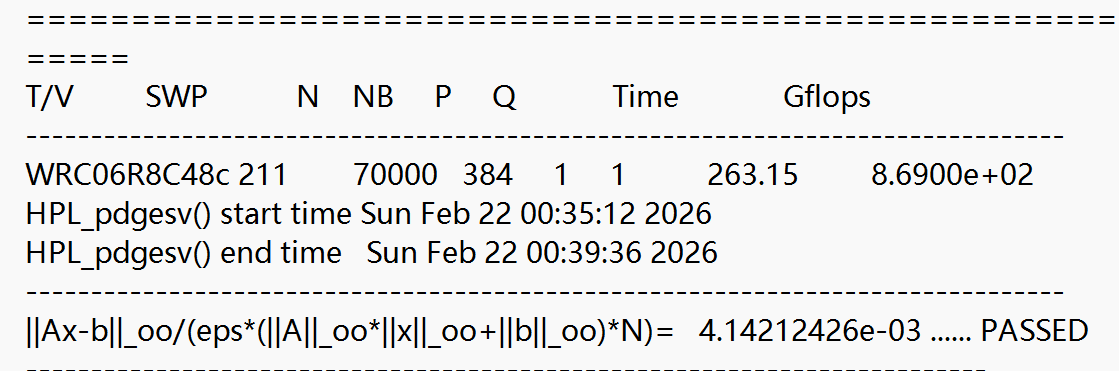
\includegraphics[width=0.8\linewidth]{figures/HPLLOG.png}
    \caption{Performance result of the CPU HPL test}
    \label{fig:hpl reult}
\end{figure}



\subsubsection{GPU Evaluation Results}
\ 

First, we configured the HPL test of the GPU based on experience and found that our test results were not good. 
Then considering that we are using AMD processors, we decided to learn the binary packages that AMD uses. 
Figure \ref{fig:hpl gpu reult} shows the best profile for the performance test with $N{=}36864$, $NB{=}1024$, $P\times Q{=}1\times1$.
Finally, we can get the efficiency is
\begin{equation}
    \text{Efficiency} {=}\frac{\text{Peak of HPL}}{\text{Theoretical Peak }} {=}\frac{\text{632.1 Gflops}}{\text{689 Gflops  }}{\approx}91.74\%
\end{equation}

\begin{figure}[!htb]
    \centering
    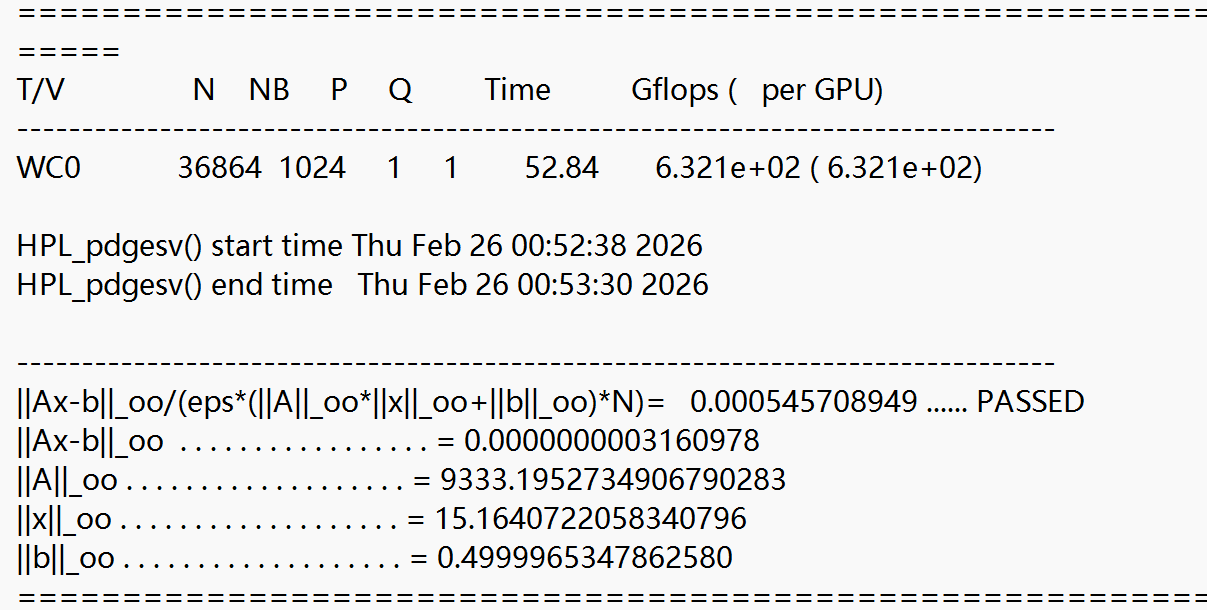
\includegraphics[width=0.8\linewidth]{figures/HPLGPU.png}
    \caption{Performance result of the single GPU HPL test}
    \label{fig:hpl gpu reult}
\end{figure}

\subsection{Summary}
\ 


To sum up, we can see that in HPL testing, in addition parameters $N$, $NB$, $P\times Q$, affecting the test results, different BLAS libraries and compilers perform differently on specific hardware. 
In the end, our \textbf{CPU efficiency and  GPU efficiency all reached about $91.74\%$}.

\clearpage

\newpage
\section{HPCG Test and Optimization}
This section focuses on the analysis and evaluation of HPCG. 
All the test results presented  are derived from the same hardware platform and software configuration for HPL, as detailed in Table \ref{tab:HPLHard} and Table \ref{tab:hpl software}.

\subsection{Analysis of HPCG}
\ 

The High Performance Conjugate Gradient (HPCG) benchmark is a key tool for assessing the performance of high-performance computing (HPC) systems, particularly in simulating real-world
computational workloads.
Unlike traditional benchmarks such as HPL, which mainly measure
floating-point operations through dense matrix multiplication, HPCG focuses on solving large sparse linear systems. 
These systems are derived from the discretization of a three-dimensional partial differential equation (PDE) that simulates a heat diffusion problem with zero Dirichlet boundary conditions.

At the heart of HPCG is the preconditioned conjugate gradient (PCG) method, which necessitates efficient handling of sparse matrix operations, optimized memory bandwidth, and parallel
computation across distributed systems. 
The global problem is defined on a three-dimensional grid
with dimensions $ (nx \times npx) \times (ny \times npy) \times (nz \times npz) $, where $nx$, $ny$, and $nz$ represent the local subgrid sizes in the $x$, $y$, and $z$ dimensions, respectively, assigned to each MPI process. 
The values $npx$, $npy$, and $npz$ denote the number of processes in each corresponding dimension. 
These values are automatically computed during the HPCG setup phase but can also be manually specified in the input file ``hpcg.dat" or provided as command-line arguments.

The HPCG benchmark consists of three critical computational kernels, each integral to evaluating modern supercomputer architectures:
\begin{enumerate}
    \item Sparse Matrix-Vector Multiplication (SpMV): The core computational task of HPCG, SpMV is computationally intensive and central to the benchmark’s performance evaluation.
    \item Symmetric Gauss-Seidel (SymGS) Relaxation: This serves as the essential preconditioning technique for the conjugate gradient method, enhancing the efficiency of the iterative solution process.
    \item  Conjugate Gradient Method: The iterative approach used to solve the large-scale sparse linear systems, making it a crucial component of HPCG’s overall performance.   
\end{enumerate}

These kernels are commonly found in scientific computing applications, such as computational fluid dynamics and electromagnetic simulations. 
They present significant challenges for system bandwidth and fine-grained parallel efficiency, making them indispensable for benchmarking modern HPC architectures.

\subsection{Performance Optimization Methods}
\ 

\subsubsection{Modification of ``HPCG.dat"}
\ 

By modifying the configuration parameters in the ``HPCG.dat" file, the optimization of the standard HPCG benchmark can be significantly impacted. 
The file contains two key sections that can be adjusted to improve performance: the problem size (specifically, the matrix size) and the runtime.
Adjusting the matrix size can have a major effect on performance.   

\begin{enumerate}
    \item \textbf{Matrix Size:} The matrix size defines the scale of the problem and is directly related to the global dimensions of the discretized computation grid. 
    By adjusting the local subgrid dimensions $(nx, ny, nz)$ and the number of subgrids in each dimension $(npx, npy, npz)$, the workload assigned to each MPI process can be optimized. 
    A larger matrix size generally increases computational complexity, which improves the scalability and performance of the benchmark on a large number of processors. 
    However, excessively large problem sizes may lead to memory limitations or imbalanced workload distribution between processes.
    Therefore, careful consideration of these parameters is essential for achieving optimal performance.
    \item \textbf{Runtime:} The runtime is another important parameter that influences the performance of the HPCG benchmark. 
    A longer runtime allows for more thorough testing of the system’s ability to handle sustained computational load. While a longer runtime provides a better measure of the system’s long-term stability and computing capacity, excessively long runtimes may lead to diminishing returns in performance due to hardware bottlenecks. 
    Therefore, choosing an appropriate runtime is essential to strike a balance between accuracy and benchmark duration. 
    In addition to the size of the topic scale, the shortest running time should be set to ensure the long enough running time of the system.
    Optimizing the matrix size and runtime in the ``HPCG.dat" file is crucial for fine-tuning benchmark performance, ensuring that the results reflect the system’s true capabilities.
    These modifications help with better load distribution, reduced memory overhead, and improved overall efficiency in parallel computing environments.
\end{enumerate}




\subsubsection{Third-Party Library for HPCG}
\ 

\begin{figure}[!htb]
    \centering
    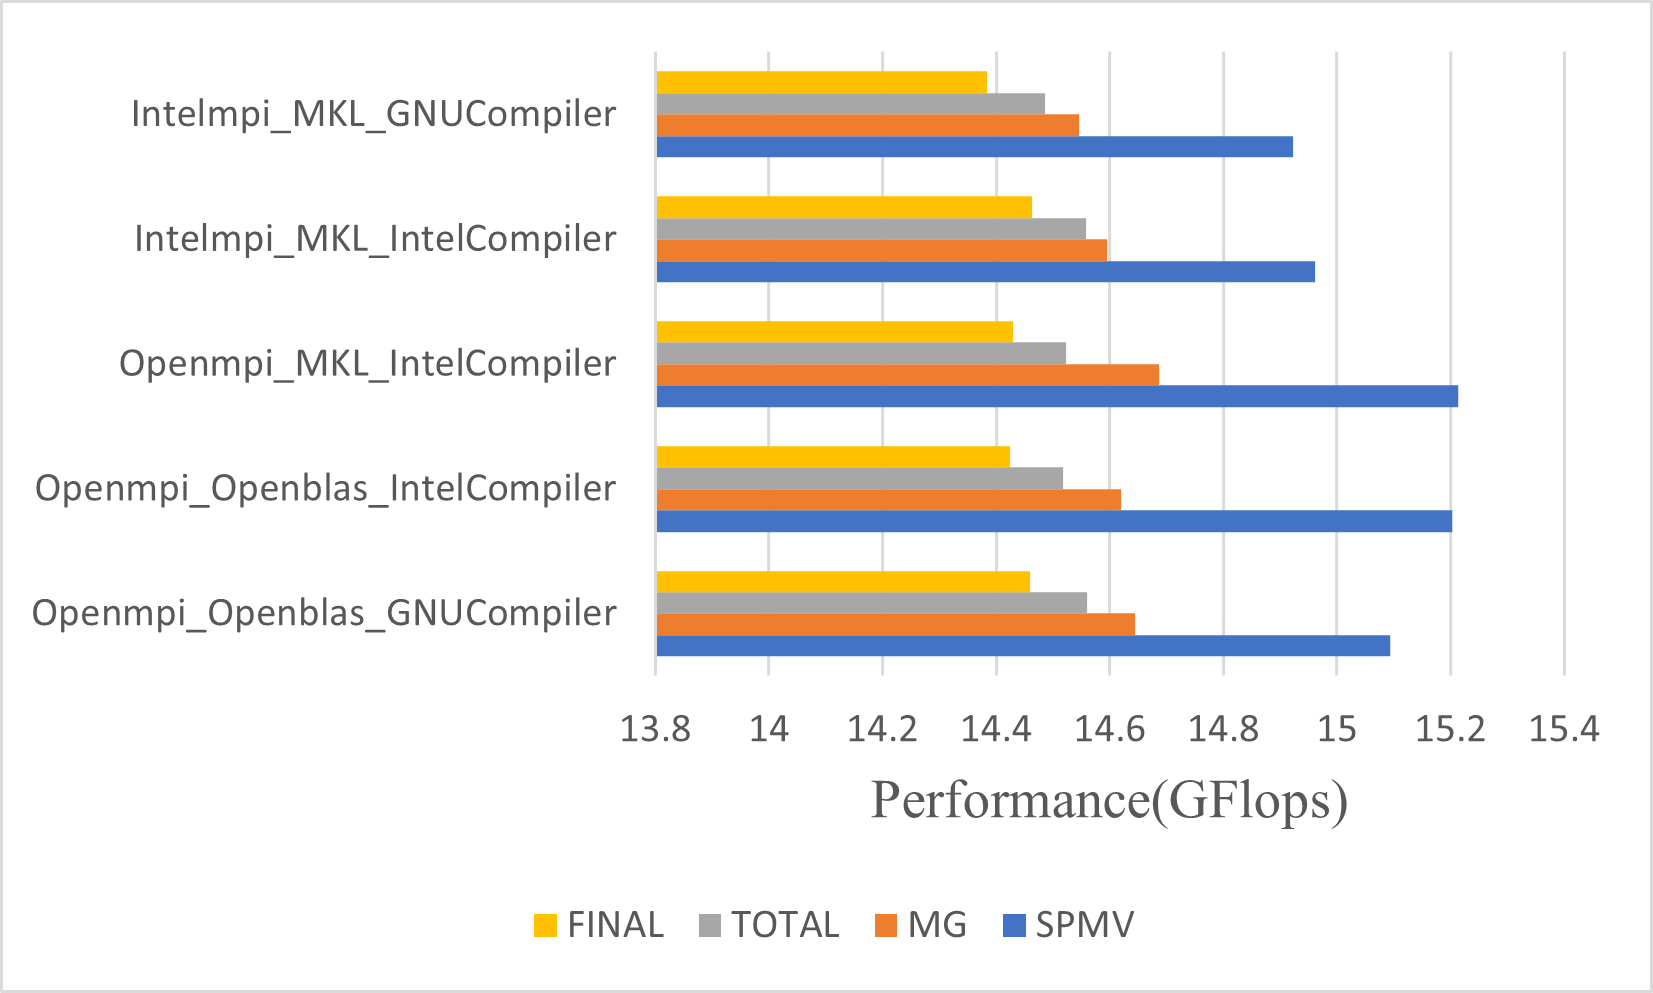
\includegraphics[width=0.8\linewidth]{figures/third party.png}
    \caption{Performance results for different third-party library settings in standard HPCG Benchmark}
    \label{fig:hpcg third party}
\end{figure}

For the standard HPCG benchmark, there are several third-party libraries available that can enhance performance. 
Key libraries include those for MPI and BLAS.
The commonly used MPI libraries are MPICH, OpenMPI, and Intel MPI (IMPI). 
These libraries handle the communication between different processes in a distributed computing environment.
For BLAS, several implementations are available, such as MKL (Intel Math Kernel Library), OpenBLAS, and Atlas.
BLAS libraries are crucial for performing optimized linear algebra operations on the CPU, which form a significant part of the HPCG computation.
After testing, we chose OpenBLAS and MKL as the BLAS libraries, while OpenMPI and Intel MPI were selected as the MPI libraries for communication.
The matrix size used in our experiments is set to $(160  \times 160  \times 128)$ and the runtime is fixed at 1800 seconds, which corresponds to the optimal parameter setting in Figure \ref{fig:hpcg third party}. 

% Please add the following required packages to your document preamble:
% \usepackage{subfig}



\subsubsection{Parallelization Paradigms for HPCG}
\ 

In this subsection, we explore three different configurations for the standard HPCG benchmark: MPI alone,  OpenMP alone, and  both MPI and OpenMP together. 
These configurations allow us to compare the performance of the standard HPCG benchmark under different parallelization paradigms and understand the impact of each parallelization method.
The matrix size used in our experiments is set to $(160  \times 160  \times 128)$, with the runtime fixed at
 1800 seconds. 
The third-party libraries used are OpenMPI and OpenBLAS, and the GNU Compiler is employed for compilation.

% Please add the following required packages to your document preamble:
% \usepackage{subfig}
\begin{figure}[!htb]
    \centering
    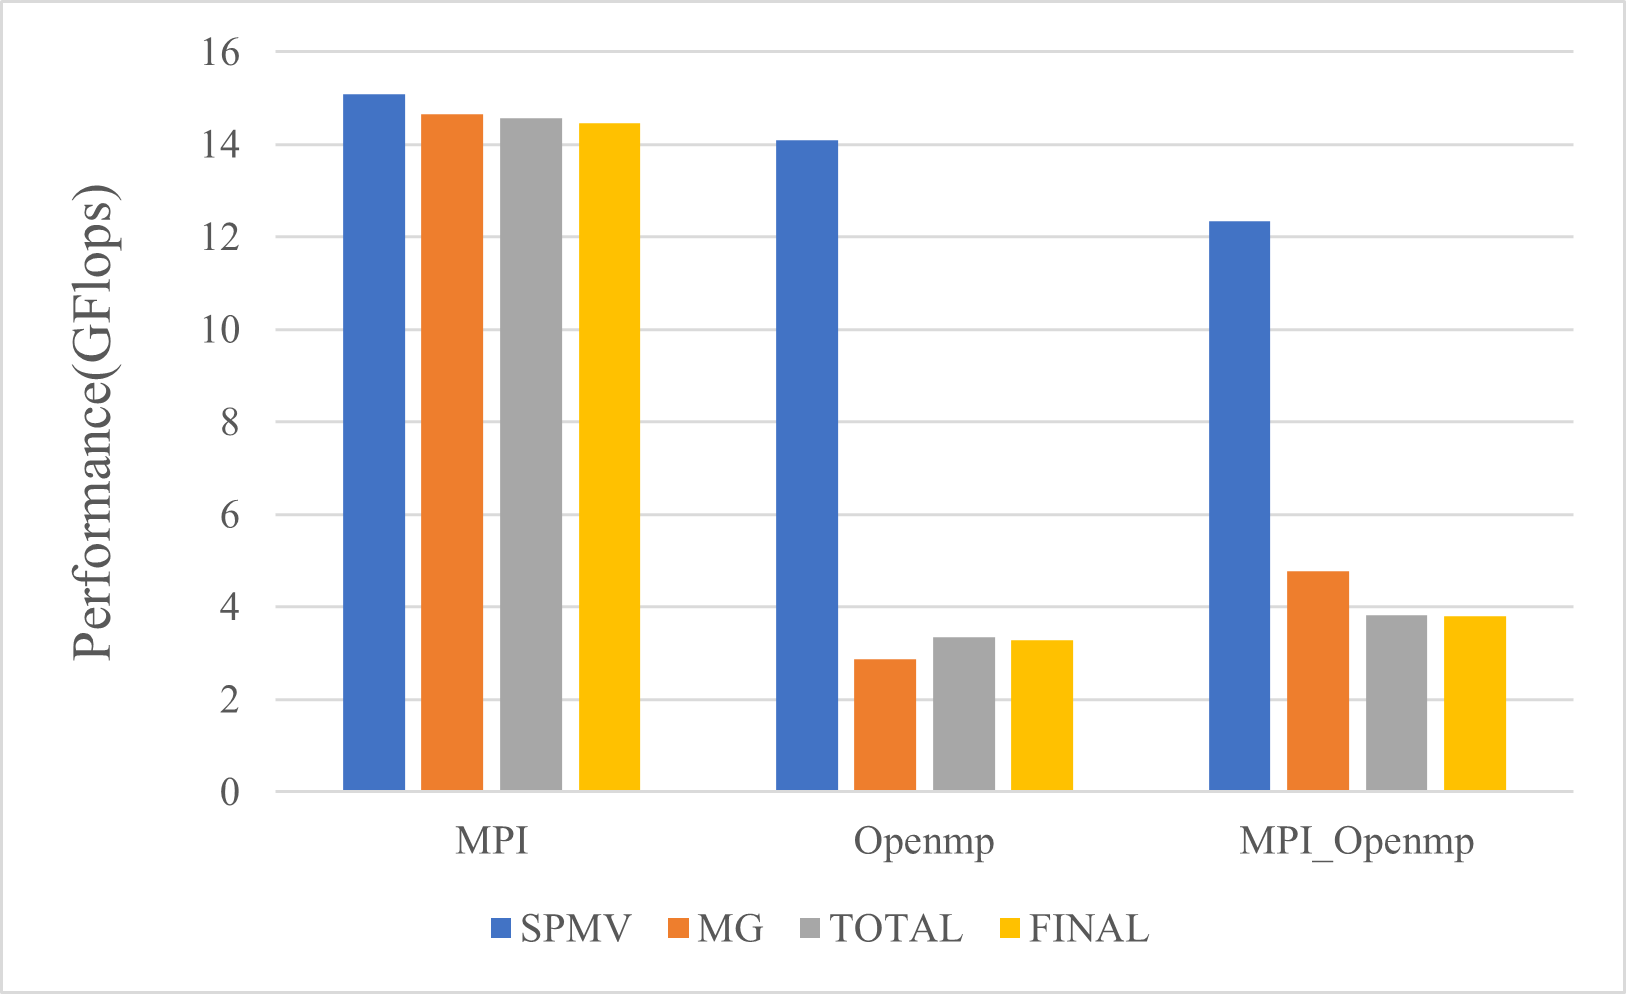
\includegraphics[width=0.8\linewidth]{figures/hpcg-mpi.png}
    \caption{Performance results for different Parallelization Paradigm settings in standard HPCG Benchmark}
    \label{fig:hpcg mpi}
\end{figure}

Based on the results of the experiments, as shown in Figure \ref{fig:hpcg mpi}, we observed that the configuration using MPI alone achieved the best performance across all tested machines. 
This configuration allowed the standard HPCG benchmark to fully utilize the distributed memory capabilities of the system, with each MPI process handling a portion of the problem.
The communication overhead, though present, was minimized due to the high efficiency of MPI in handling large-scale parallel problems.
In contrast, using OpenMP alone resulted in lower performance, primarily due to the limited scalability on a single-node setup. 
Although OpenMP effectively leveraged multicore CPUs, it was constrained by memory bandwidth and the relatively limited computational power available within a single node.
The hybrid  configuration performed well on multi-node systems, but the performance improvement was not as significant as expected. 
This is likely due to suboptimal load balancing between MPI and OpenMP, where the communication overhead between processes overshadowed the benefits of multi-threading within nodes. 
Moreover, hybrid configurations often require fine-tuning to achieve maximum performance, especially with larger problem sizes, which can result in a less straightforward optimization process.

\subsubsection{Hybrid Version of HPCG}
\ 

To further optimize performance, a hybrid approach can be applied to the HPCG benchmark, integrating CUDA for GPU acceleration. 
This allows the GPU’s floating-point performance to be exploited without altering the basic conjugate gradient (CG) algorithm or preconditioner algorithm.
The GPU’s parallel processing power is harnessed to significantly speed up matrix operations, which are a critical part of the HPCG benchmark.
In this hybrid version, the matrix is analyzed, reordered, and the computational workload is split between the CPU and GPU. 
The CPU handles portions of the matrix that are better suited for traditional processors, while the GPU is responsible for the portions that benefit most from parallel computation capabilities. 
This approach allows the hybrid version to capitalize on the strengths of both the CPU and GPU, optimizing performance for large-scale computations.
Fine-tuning the ratio of CPU to GPU workload is essential to achieve optimal performance. 
By experimenting with different configurations and workloads, the ideal distribution of tasks between
CPU and GPU can be found, maximizing the overall performance of the HPCG benchmark on systems equipped with both CPU and GPU resources.
The hybrid version allows HPCG to fully utilize both CPU and GPU resources, providing an effective solution for high-performance computing systems with multi-core CPUs and GPUs.


\subsection{Experimental Results}
\ 


\subsubsection{CPU Evaluation Results}
\ 

Since our server uses an AMD CPU, using the AMD-specific HPCG benchmark allows for the full utilization of its hardware features, resulting in a more accurate performance evaluation. 
Compared to the standard HPCG benchmark, the AMD version is optimized to better reflect performance in real-world applications. 
The following describes the test experiments for the AMD-specific
HPCG benchmark.
First, We conducted experiments by using only the CPU to run the AMD-specific HPCG benchmark. 
To achieve the best performance, we tested different data scales by adjusting the matrix size in the configuration file ``HPCG.dat".
By fine-tuning the matrix size, we sought to identify the optimal configuration for CPU-based computations on our AMD hardware.
And finally we get the best performance 21.2034 GFlops with:
\begin{itemize}
    \item \textbf{Matrix Size:} $512{\times}256{\times}256$.
    \item \textbf{Number of subgrids:} $npx{=}4$, $npy{=}2$, $npz{=}2$.
    \item \textbf{runtime:} 1800s.
\end{itemize}

So, the efficiency of the CPU evaluation is
\begin{equation}
    \text{Efficiency} {=}\frac{\text{Peak of HPL}}{\text{Theoretical Peak }} {=}\frac{\text{21.2034 GFlops}}{\text{947.2 GFlops }}{\approx}2.24\%
\end{equation}

\subsubsection{GPU Evaluation Results}
\ 

For GPU evaluation, we utilized the CUDA-enabled version of the HPCG benchmark.
The version we used is provided by NVIDIA and cannot be modified. Although we attempted to analyze the source code as time permitted, it is undeniable that there is a significant gap between our understanding and the optimizations implemented in the NVIDIA-provided version. 
Therefore, our current optimizations for HPCG were primarily achieved through parameter tuning in the ``HPCG.dat" file. 
These adjustments contributed to improved performance on GPU-based computations.
After testing multiple configurations, the optimal performance achieved was 232.673 GFlops with
\begin{itemize}
    \item \textbf{Matrix Size:} $256{\times}256{\times}256$.
    \item \textbf{Number of subgrids:} $npx{=}1$, $npy{=}1$, $npz{=}2$.
    \item \textbf{runtime:} 1800s.
    \item \textbf{Number of GPUs:} 2 (Dual GPU configuration).
\end{itemize}



\begin{equation}
    \text{Efficiency} {=}\frac{\text{Peak of HPL}}{\text{Theoretical Peak }} {=}\frac{\text{232.673 GFlops}}{\text{689 GFlops}\times 2}{\approx}16.88\%
\end{equation}

\subsection{Summary}
\ 

In the HPCG tests, our \textbf{CPU efficiency reached  21.2034 GFlops with  about 2.24\% efficiency}, and  \textbf{the GPU’s computational peak reaches 232.673 GFlops with about 16.88\% efficiency}.
\newpage
% \documentclass{article}
% \usepackage[utf8]{inputenc}
% \usepackage{indentfirst}
% \usepackage{comment}
% \usepackage[table]{xcolor}
% \usepackage{multirow}
% \usepackage{array}
% \usepackage[margin=1in]{geometry}
% \usepackage{caption}
% \captionsetup[table]{skip=10pt}
% \usepackage{float}
% \usepackage{listings}
% \usepackage{xcolor}
% \usepackage{enumitem}

% \begin{titlepage}
%     \centering
%     \vspace*{\fill}
%     {\Huge \textbf{Embodied World Model Optimization Proposal}}
%     \vspace{1.5cm}
%     \vspace*{\fill}

% \end{titlepage}

% \newpage

% \begin{center}
%     {\LARGE \textbf{Optimization for UnifoLM-WMA-0 Inference}}
% \end{center}
\section{Optimization for UnifoLM-WMA-0 Inference}
\subsection{Introduction}
\

\begin{comment}
宇树科技研发的 UnifoLM-WMA 是一款将生成式世界模型与动作策略模型深度融合的具身智能基础模型，
它通过模拟物理后果的“心理排演”机制，使机器人具备了高保真环境预测与复杂任务决策能力；
但在实际部署中，由于该模型涉及较高维度的连续视频合成与密集的迭代状态去噪过程，其推理计算量巨大，
已成为制约机器人实现高频实时控制与长时程规划的核心算力瓶颈。

在本次竞赛中，我们的核心目标是在保证每个 case 下模型 generated video 与组委会提供的基准视频之间
的 psnr 值大于 25 的前提下缩短 unifolm-wma 的推理时间. 对此，我们团队尝试和探索了包括 NUMA Affinity Optimzation, Mixed Precision, I/O Improvments, 
FlashAttention Recomputation, DeepCache Implement 在内的 5 种优化方法，这一部分详细内容请参见 section3.

服务器 A 是我们最终参赛并用于验证最后优化结果的服务器，服务器 B 是我们团队刚开始进行具身智能优化时使用的服务器，但在经过多种尝试之后，该
服务器的 Baseline test 并不符合组委会要求，在该服务器上的测试数据用于辅助我们分析各优化方法的利弊. 关于服务器 A 和 B 的具体信息，请参考 sectioin 5.1.

在尝试多种优化方法后，为了保证测试结果符合赛题要求，我们最终在服务器 A 上采取了 Mixed Precision，I/O improvments 和 FlashAttention Recomputation 三种优化方法相融合的方式作为最终的优化方案，
其优化效果请参见 Section 5.2.
\end{comment}
UnifoLM-WMA, developed by Unitree Robotics, is an embodied artificial intelligence foundation model that deeply integrates a generative world model with an action policy model \cite{unifolm-wma-0}.
By leveraging a ``mental rehearsal" mechanism to simulate physical consequences, it equips robots with high-fidelity environmental prediction and complex task decision-making capabilities. 
However, practical deployment faces a critical computational bottleneck: the massive inference load driven by high-dimensional continuous video synthesis and intensive iterative state denoising severely restricts high-frequency real-time control and long-horizon planning.

In this competition, our primary objective is to accelerate the inference speed of UnifoLM-WMA while strictly maintaining a Peak Signal-to-Noise Ratio (PSNR) above 25(compared to the committee's reference videos) across all test cases.
To achieve this, our team explored five distinct optimization strategies: NUMA Affinity Optimization, Mixed Precision, I/O Improvements, FlashAttention Recomputation, and DeepCache Implementation. 
A detailed discussion of these methods is provided in Section \ref{sec:unif methods}.



Our empirical evaluation is conducted across two hardware environments (detailed in Section \ref{sec:unif exp envir}), named as ``Server A" and ``Server B".
``Server B" was utilized during our initial exploration phase; although its PSNR performance of the baseline test did not meet the committee's formal requirements, the data gathered from it is instrumental in analyzing the specific trade-offs and efficacies of each optimization technique. 
``Server A" serves as our definitive submission platform for validating the final results.


To ensure robust compliance with the competition's rigorous standards, we ultimately deployed a synergistic optimization pipeline on ``Server A", integrating Mixed Precision, I/O Improvements, and FlashAttention Recomputation. 
The comprehensive performance results of this final solution are presented in Section \ref{sec:unif exp reult}.

To quantitatively assess the impact of these optimization strategies on inference performance, we conducted baseline and optimized evaluations on both ``Server A" and ``Server B", with statistical comparisons of PSNR and inference time. 
The baseline environment was strictly configured following the official guidelines provided by the organizing committee and the Unitree code repository.

\textbf{On ``Server A", we analyzed 20 test cases. 
The baseline averaged 39.72 dB in PSNR and 578.2 seconds in inference time. 
After optimization, the average inference time dropped to 404.5 seconds, yielding a mean speedup of 1.407$\times$, while the post-optimization PSNR remained above 39 dB, showing negligible fluctuation from the baseline.} 
All individual cases maintained a PSNR above the required 25 dB threshold.

\textbf{On ``Server B", although the baseline PSNR averaged only 21.43 dB (below the 25 dB requirement), the PSNR values remained virtually unchanged after optimization, averaging approximately 21.4 dB. Concurrently, the inference time was reduced from 1296.1 seconds to 336.9 seconds, achieving an average speedup of 3.822$\times$.} Given the consistent PSNR, the speedup measurements obtained on ``Server B" retain meaningful comparative value for assessing the relative effectiveness of different optimization methods.





\subsection{Optimization Methods}\label{sec:unif methods}
\
\begin{figure}
    \centering
    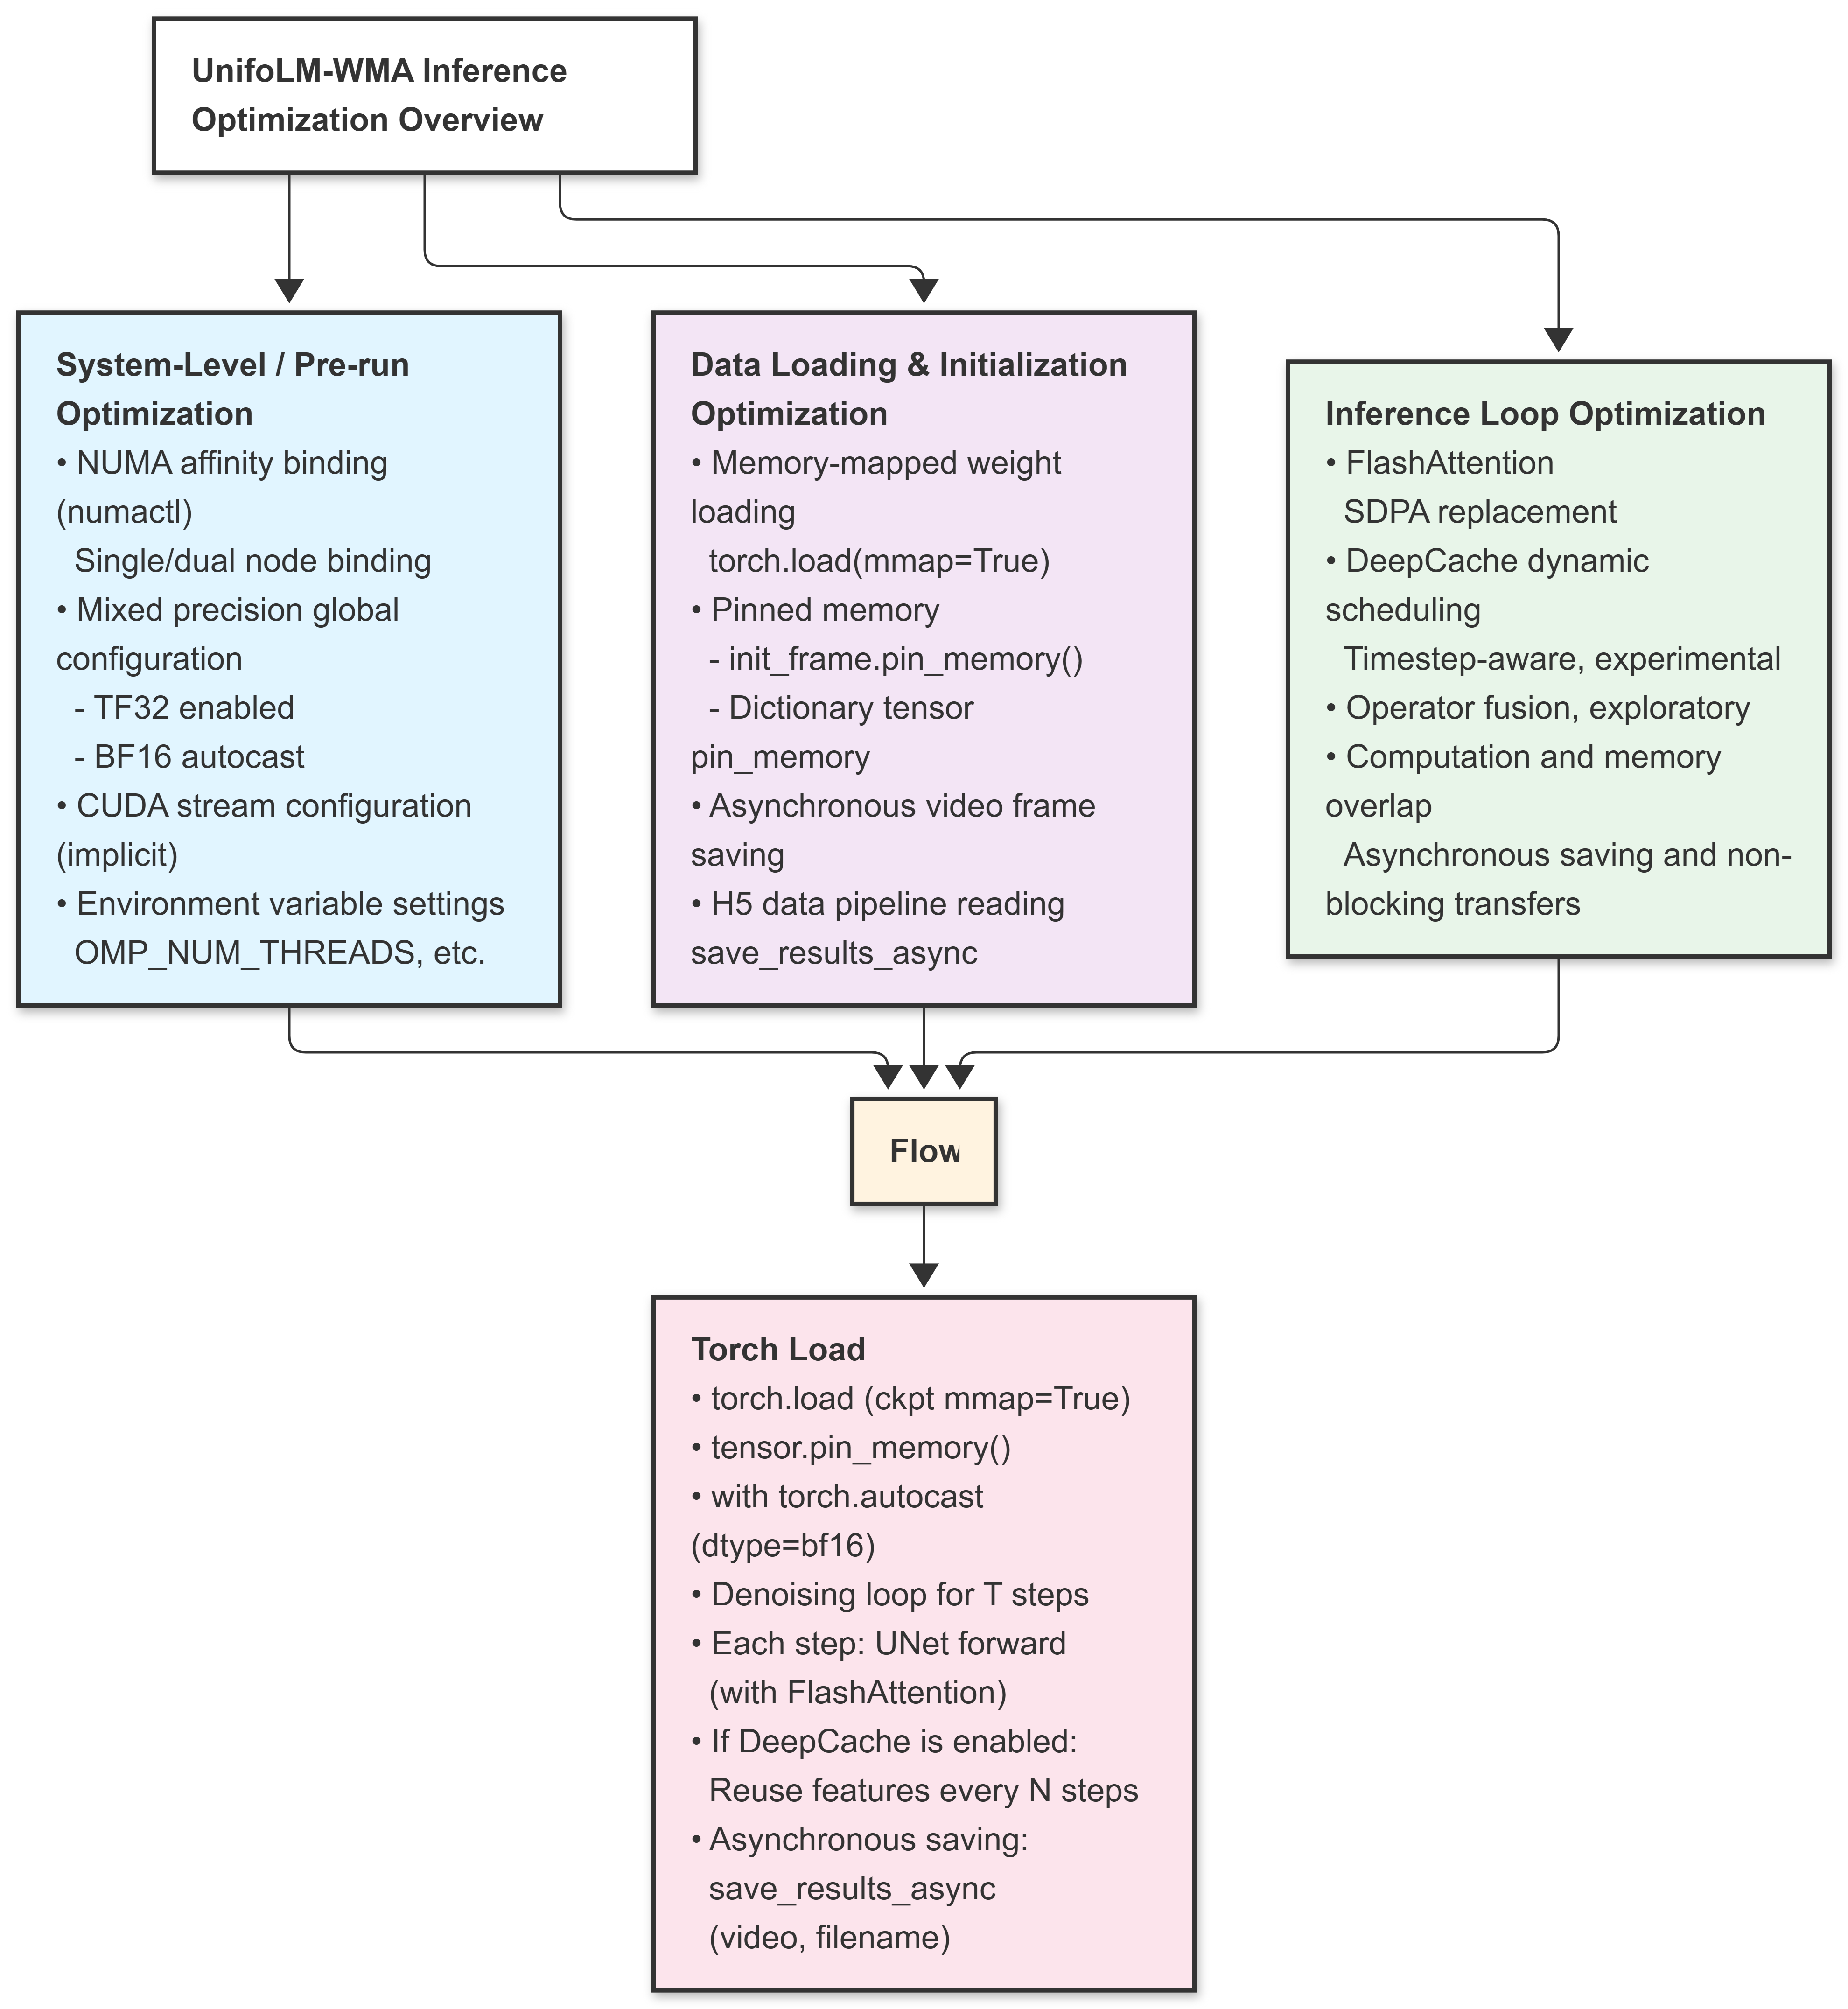
\includegraphics[width=0.8\linewidth]{Br_ Memory Flow-2026-03-02-102603.png}
    \caption{Workflow Optimization Map}
    \label{fig:unifo overview}
\end{figure}


To systematically enhance the inference efficiency of UnifoLM-WMA, we designed a collaborative optimization scheme across three levels, as illustrated in Figure \ref{fig:unifo overview}.

(1) System-Level Pre-configuration

Prior to model execution, NUMA affinity is enforced using the numactl tool to ensure that CPU memory accesses and GPU resources are confined to the same physical node, thereby eliminating latency overhead incurred by cross-node communication. 
Concurrently, global mixed-precision settings are enabled: TF32 format is permitted to accelerate matrix operations, while BF16 automatic mixed precision (autocast) is applied in core computational regions to reduce memory footprint and data transfer volume.

(2) Data Loading and I/O Optimization

To address bottlenecks associated with loading large-scale model weights and input data, we employ memory-mapped loading via torch.load(mmap=True), eliminating redundant CPU memory copies. Input images and tensors are pinned to page-locked memory using .pin memory() to accelerate CPU-to-GPU transfer efficiency. For H5-format input data, a pipelined reading mechanism is constructed to minimize I/O waiting. For video frame saving, an asynchronous saving function save results async is designed to offload post-processing and disk write operations to background threads, allowing the main thread to proceed directly to the next inference iteration.

(3) Inference Loop Optimization

Within the core denoising loop, FlashAttention replaces standard attention implementations to reduce memory read/write overhead. The DeepCache scheduling strategy remains under experimental investigation to determine optimal parameter configurations: through a timestep-aware caching mechanism, deep features are reused every N steps, bypassing full U-Net forward passes and thereby reducing computational load. Computation and storage overlap is achieved through asynchronous saving and non-blocking transfers, ensuring sustained GPU computation during I/O operations. Operator fusion is currently in the exploratory phase and is considered a direction for future optimization.

Overall Data Flow: After model weights are loaded via memory mapping, input data is transferred to the GPU through pinned memory. Within the BF16 automatic mixed-precision context, a T-step denoising loop is executed, where each U-Net forward pass integrates FlashAttention; if DeepCache is enabled, features are reused at set intervals. The generated video is ultimately saved to disk via the asynchronous function, achieving substantial overlap between computation and I/O.

%todo：overview的图和说明。
% 在 6.2 部分


\subsubsection{NUMA Affinity Optimization}
\

\begin{comment}
从 NUMA 架构的角度来看，服务器 A 是单 node 结构，服务器 B 是双 node 架构. 该优化方法针对以服务器 B 为代表的多 node NUMA 架构机器.

我们通过使用 numactl 工具将脚本的运行和 CPU 调度，GPU 使用都在同一个 node 节点上进行，避免跨 node 节点访问，预计提速 10% 左右.

在双路 NUMA 架构中，CPU、内存与 GPU 被物理分割在两个独立的节点（Socket）中。当计算进程运行在一个节点，却需要调用另一个节点的内存或 GPU 时，
数据必须跨越节点间总线（如 QPI/UPI）。这种跨节点访问会引入较高的延迟，并受限于总线带宽上限，在大规模推理任务中极易引发数据拥塞，成为性能瓶颈。、
使用 numactl 工具可以建立“硬件局部性（Hardware Locality）”。通过操作系统调度，强制将计算进程、物理内存和目标 GPU 锁定在同一个物理节点内。
这种方式确保了任务与其所需资源在物理拓扑上完全对齐，消除了跨节点通信产生的多余开销，从而显著提升系统的整体吞吐量，提高模型推理速度.\textbf{}

Server B Baseline Test Results
Server B Taking NUMA Affinity Optimization's Results
NUMA Affinity OPtimization's performance
\end{comment}

\begin{table}[!htbp]
    \centering
    \small
    \renewcommand{\arraystretch}{1.0}
    \caption{Impact of NUMA Affinity Optimization on Server B Inference,where the baseline performance is detailed in Section \ref{sec:unif exp reult}. And, the values in the parentheses of the ``Test Time" and ``Test PSNR" columns respectively represent the speedup ratio relative to the baseline time and the difference to baseline PSNR.}
    \label{tab:server_b_numa}
    \begin{tabular}{|>{\centering\arraybackslash}m{6cm}|c|c|c|}
        \hline
        \rowcolor{yellow} \textbf{Scenario} & \textbf{Case} & \textbf{Test Time} & \textbf{Test PSNR} \\ \hline
        
        \multirow{4}{*}{unitree\_g1\_pack\_camera} 
        & 1 & 19m26.800s / 1166.800 s (1.230$\times$)& 18.5229(0) \\ \cline{2-4}
        & 2 & 19m25.073s / 1165.073 s(1.236$\times$) & 18.5432(0)\\ \cline{2-4}
        & 3 & 19m20.739s / 1160.739 s(1.241$\times$)& 19.9578(0) \\ \cline{2-4}
        & 4 & 19m22.388s / 1162.388 s(1.236$\times$) & 17.7746(0)\\ \hline
        
        \multirow{4}{*}{unitree\_z1\_stackbox}     
        & 1 & 20m54.452s / 1254.452 s(1.238 $\times$) & 23.9826(0)\\ \cline{2-4}
        & 2 & 20m53.071s / 1253.071 s(1.243$\times$) & 20.0572(0)\\ \cline{2-4}
        & 3 & 20m53.853s / 1253.853 s(1.240$\times$) & 21.7059(0)\\ \cline{2-4}
        & 4 & 20m52.502s / 1252.502 s(1.243 $\times$) & 25.2775(0)\\ \hline
        
        \multirow{4}{*}{unitree\_z1\_dual\_arm\_stackbox\_v2} 
        & 1 & 19m33.918s / 1173.918 s(1.234$\times$) & 20.0181(0)\\ \cline{2-4}
        & 2 & 19m29.337s / 1169.337 s(1.238$\times$) & 18.8915(0)\\ \cline{2-4}
        & 3 & 19m32.557s / 1172.557 s(1.236$\times$) & 18.8271(0)\\ \cline{2-4}
        & 4 & 19m31.043s / 1171.043 s(1.237 $\times$) & 19.3431(0)\\ \hline
        
        \multirow{4}{*}{unitree\_z1\_dual\_arm\_stackbox}     
        & 1 & 13m5.162s / 785.162 s (1.226$\times$)& 22.8169(0)\\ \cline{2-4}
        & 2 & 13m5.668s / 785.668 s (1.229$\times$)& 24.5789(0)\\ \cline{2-4}
        & 3 & 13m5.123s / 785.123 s (1.225$\times$)& 26.2675(0)\\ \cline{2-4}
        & 4 & 13m4.947s / 784.947 s (1.228$\times$)& 25.3952(0)\\ \hline
        
        \multirow{4}{*}{unitree\_z1\_dual\_arm\_cleanup\_pencils} 
        & 1 & 14m31.863s / 871.863 s(1.231$\times$) & 21.2321(0)\\ \cline{2-4}
        & 2 & 14m32.574s / 872.574 s(1.234$\times$)& 22.5411(0)\\ \cline{2-4}
        & 3 & 14m33.037s / 873.037 s(1.229$\times$) & 19.9960(0)\\ \  cline{2-4}
        & 4 & 14m32.806s / 872.806 s(1.234$\times$) & 22.8648(0)\\ \hline
        \textbf{Average}&-& 17m45.346s / 1065.346s(1.234$\times$)&21.4297(0) \\ \hline
    \end{tabular}
\end{table}

From the perspective of Non-Uniform Memory Access (NUMA) topology, ``Server A" features a single-node structure, whereas ``Server B" employs a dual-node architecture. 
The optimization strategy detailed herein is specifically designed for multi-node NUMA systems, as exemplified by ``Server B".

In a dual-socket NUMA configuration, CPUs, memory, and GPUs are physically partitioned across distinct hardware nodes (sockets).
Consequently, when a computational process residing on one node attempts to access memory or GPU resources located on the other, the data must traverse the interconnect bus (e.g., QuickPath Interconnect or UltraPath Interconnect). 
This cross-node communication introduces substantial latency and is strictly constrained by the bandwidth limits of the bus. 
During intensive, large-scale inference tasks, such architectural constraints frequently induce data congestion, manifesting as a critical performance bottleneck.

To mitigate this bottleneck, we utilize the numactl utility to enforce strict hardware locality. 
By leveraging OS-level scheduling, this approach confines script execution, CPU scheduling, memory allocation, and target GPU utilization entirely within a single physical node. 
This strategy guarantees a precise topological alignment between computational tasks and their requisite hardware resources. 
By circumventing the redundant overhead associated with cross-node communication, this method substantially enhances the overall system throughput and accelerates model inference, \textbf{resulting in an approximately 23.4\% reduction in inference time as shown in Table \ref{tab:server_b_numa}(the baseline test on ``Server B" is shown in Table \ref{tab:server_b_baseline}).} Since NUMA binding operates strictly as an OS-level optimization for hardware resource scheduling, it does not interfere with the model's underlying mathematical logic. \textbf{Consequently, the PSNR of the generated videos remains unaffected, yielding a mean variance of zero.}



%caption第一个表格解释了，后续就不再赘述；PSNR的变化平均值没写。
% done



% \begin{table}[!htbp]
%     \centering
%     \renewcommand{\arraystretch}{1.0}
%     \caption{Detailed Efficiency Analysis of NUMA Affinity Optimization on Server B}
%     \label{tab:numa_eval}
%     \begin{tabular}{|>{\centering\arraybackslash}m{5.8cm}|c|c|c|}
%         \hline
%         \rowcolor{yellow} \textbf{Scenario} & \textbf{Case} & \textbf{Diff Time} & \textbf{Speedup} \\ \hline
        
%         \multirow{4}{*}{unitree\_g1\_pack\_camera} 
%         & 1 & \textcolor{diffgreen}{\textbf{-268.242}} & 1.230 \\ \cline{2-4}
%         & 2 & \textcolor{diffgreen}{\textbf{-275.394}} & 1.236 \\ \cline{2-4}
%         & 3 & \textcolor{diffgreen}{\textbf{-279.310}} & 1.241 \\ \cline{2-4}
%         & 4 & \textcolor{diffgreen}{\textbf{-274.493}} & 1.236 \\ \hline
        
%         \multirow{4}{*}{unitree\_z1\_stackbox}     
%         & 1 & \textcolor{diffgreen}{\textbf{-298.783}} & 1.238 \\ \cline{2-4}
%         & 2 & \textcolor{diffgreen}{\textbf{-304.013}} & 1.243 \\ \cline{2-4}
%         & 3 & \textcolor{diffgreen}{\textbf{-300.515}} & 1.240 \\ \cline{2-4}
%         & 4 & \textcolor{diffgreen}{\textbf{-304.661}} & 1.243 \\ \hline
        
%         \multirow{4}{*}{unitree\_z1\_dual\_arm\_stackbox\_v2} 
%         & 1 & \textcolor{diffgreen}{\textbf{-274.348}} & 1.234 \\ \cline{2-4}
%         & 2 & \textcolor{diffgreen}{\textbf{-278.736}} & 1.238 \\ \cline{2-4}
%         & 3 & \textcolor{diffgreen}{\textbf{-277.114}} & 1.236 \\ \cline{2-4}
%         & 4 & \textcolor{diffgreen}{\textbf{-277.036}} & 1.237 \\ \hline
        
%         \multirow{4}{*}{unitree\_z1\_dual\_arm\_stackbox}     
%         & 1 & \textcolor{diffgreen}{\textbf{-177.274}} & 1.226 \\ \cline{2-4}
%         & 2 & \textcolor{diffgreen}{\textbf{-180.053}} & 1.229 \\ \cline{2-4}
%         & 3 & \textcolor{diffgreen}{\textbf{-176.711}} & 1.225 \\ \cline{2-4}
%         & 4 & \textcolor{diffgreen}{\textbf{-179.074}} & 1.228 \\ \hline
        
%         \multirow{4}{*}{unitree\_z1\_dual\_arm\_cleanup\_pencils} 
%         & 1 & \textcolor{diffgreen}{\textbf{-201.198}} & 1.231 \\ \cline{2-4}
%         & 2 & \textcolor{diffgreen}{\textbf{-204.318}} & 1.234 \\ \cline{2-4}
%         & 3 & \textcolor{diffgreen}{\textbf{-199.552}} & 1.229 \\ \cline{2-4}
%         & 4 & \textcolor{diffgreen}{\textbf{-204.002}} & 1.234 \\ \hline
%     \end{tabular}
% \end{table}




\subsubsection{Mixed Precision}
\

\begin{comment}
混合精度优化的基本原理在于，深度神经网络对数值的微小误差并不敏感，不需要极高的小数精度也能保持输出结果的准确。
在模型推理时，将常规的 32 位浮点数（FP32）替换为 16 位的 BF16 或 TF32 格式，最直接的效果是将模型参数和计算时产生的数据总量缩减了一半。
数据变小后，系统在内存和 GPU 之间搬运数据的负担大幅减轻，直接缓解了数据传输慢导致的 I/O 堵塞问题，也提高了数据传输的速度。 
BF16 通过截断尾数保留了与 FP32 相同的指数位宽（即维持了数值的动态范围），而 TF32 则在内部计算时利用了低位宽乘法的硬件优势。
同时，由于单笔计算的数据变短了，现代 GPU 内部的计算单元可以在同一个时钟周期内并行处理更多的浮点运算，让现有的计算资源发挥出成倍的吞吐量。
简而言之，混合精度通过合理舍弃多余的小数精度，换取了更小的显存占用和更快的数据流转，
在确保生成视频质量（PSNR）损失较低的情况下，切实提升整体的推理速度。

在具体优化上，可以分为 3 个可选的独立部分：

一是在全局计算后端的环境配置中，通过置位 torch.backends.cuda.matmul.allow_tf32 = True 
与 torch.backends.cudnn.allow_tf32 = True 开启硬件级的 TF32（TensorFloat-32）加速机制。该指令允许 CUDA 和 cuDNN 核心库在执行矩阵乘法和卷积操作时，
自动将输入的 FP32 数据无缝转换为 TF32 格式。TF32 格式巧妙地截取了 FP32 的 8 位指数域以保证同样的动态范围防止溢出，同时保留了 FP16 的 10 位尾数域以满足模型所需的精度。

二是在核心的扩散去噪循环（如动作序列向量生成，视频序列帧生成）中引入了基于 bfloat16 的自动混合精度（AMP）推理架构。通过使用 torch.autocast(device_type="cuda", dtype=torch.bfloat16) 上下文管理器，
构建一个智能的精度调度机制。该机制能够动态识别计算图中的算子特征：针对计算密集型算子（如 Linear、Conv2d），其输入会被自动转换为 bfloat16 并送入 Tensor Core 极速计算；
而对于对数值精度极度敏感的算子（如 LayerNorm、Softmax），则严格保留 FP32 格式以维持数值稳定性。

三是对 unifolm_wma_dual.ckpt 和 ViT-H-14 模型的权重进行短精度截断再从 CPU 内存移进显存，实现 PCIe 总线在传输模型权重时数据运输压力减半.

在服务器 A 上，我们尝试过同时采取上述 3 个措施进行混合精度优化，但发现会有部分 case 的 psnr 值不达标，于是在服务器 A 上，我们选择了保守的混合精度优化方案，
只采取前面两种措施（且不在世界模型生成视频序列帧的推理循环中启用混合精度）。采用该优化方法后，平均每个 case 的加速比为 1.33X，具体优化效果如下：

对于服务器 B，我们采取了激进的混合精度优化方案，同时采取上述所有优化措施，具体结果如下：

请专业，学术，简要，优雅地将这段话整理成英文材料
\end{comment}
The fundamental principle of mixed-precision optimization relies on the fact that deep neural networks are generally insensitive to minor numerical variances, allowing them to maintain output accuracy without requiring extremely high decimal precision. 
During model inference, replacing standard 32-bit floating-point (FP32) formats with 16-bit BF16 or TF32 (TensorFloat-32) formats directly halves the total data volume of model parameters and intermediate computations. 
This reduction significantly alleviates the data transfer payload between system memory and the GPU, effectively mitigating I/O bottlenecks and accelerating transmission speeds. 
Specifically, BF16 retains the same exponent width as FP32 by truncating the mantissa, thereby preserving the dynamic range; meanwhile, TF32 leverages hardware-level advantages for low bit-width multiplication during internal computations.  
Furthermore, because the individual data elements are shorter, modern GPU computing units can process a greater number of floating-point operations in parallel within a single clock cycle, multiplicatively increasing the throughput of existing hardware. 
In summary, mixed precision trades unnecessary decimal precision for a smaller memory footprint and faster data flow, tangibly improving overall inference speed while ensuring minimal degradation in the generated video quality (PSNR).

%表信息修改
\begin{table}[!htbp]
    \centering
    \small
    \renewcommand{\arraystretch}{1.0}
    \caption{Impact of Mixed Precision Optimization on Server A Inference, where the baseline performance is detailed in Section \ref{sec:unif exp reult}.}
    \label{tab:server_b_precision2}
    \begin{tabular}{|>{\centering\arraybackslash}m{6cm}|c|c|c|}
        \hline
        \rowcolor{yellow} \textbf{Scenario} & \textbf{Case} & \textbf{Test Time} & \textbf{Test PSNR} \\ \hline
        
        \multirow{4}{*}{unitree\_g1\_pack\_camera} 
        & 1 & 9m29.502s / 569.502 s (1.297$\times$) & 36.2602(0.619) \\ \cline{2-4}
        & 2 & 7m43.190s / 463.190 s (1.357$\times$) & 42.7647(9.462) \\ \cline{2-4}
        & 3 & 7m50.046s / 470.046 s (1.333$\times$) & 34.4601(-4.614) \\ \cline{2-4}
        & 4 & 7m41.468s / 461.468 s (1.365$\times$) & 33.5926(-0.535) \\ \hline
        
        \multirow{4}{*}{unitree\_z1\_stackbox}     
        & 1 & 8m13.019s / 493.019 s (1.387$\times$) & 48.3723(-0.542) \\ \cline{2-4}
        & 2 & 8m15.012s / 495.012 s (1.377$\times$) & 47.5901(6.848) \\ \cline{2-4}
        & 3 & 8m14.072s / 494.072 s (1.363$\times$) & 48.0674(-1.713) \\ \cline{2-4}
        & 4 & 8m18.593s / 498.593 s (1.364$\times$) & 47.1862(-0.075) \\ \hline
        
        \multirow{4}{*}{unitree\_z1\_dual\_arm\_stackbox\_v2} 
        & 1 & 7m48.821s / 468.821 s (1.355$\times$) & 25.2486(-0.819) \\ \cline{2-4}
        & 2 & 7m45.663s / 465.663 s (1.365$\times$) & 27.1028(-3.405) \\ \cline{2-4}
        & 3 & 8m3.851s / 483.851 s (1.326$\times$) & 32.4244(0.431) \\ \cline{2-4}
        & 4 & 7m52.203s / 472.203 s (1.351$\times$) & 34.2318(-4.998) \\ \hline
        
        \multirow{4}{*}{unitree\_z1\_dual\_arm\_stackbox}     
        & 1 & 5m32.981s / 332.981 s (1.307$\times$) & 43.8239(4.693) \\ \cline{2-4}
        & 2 & 5m32.647s / 332.647 s (1.307$\times$) & 42.1073(2.184) \\ \cline{2-4}
        & 3 & 5m33.863s / 333.863 s (1.312$\times$) & 36.0992(-0.586) \\ \cline{2-4}
        & 4 & 5m33.525s / 333.525 s (1.308$\times$) & 47.0527(5.542) \\ \hline
        
        \multirow{4}{*}{unitree\_z1\_dual\_arm\_cleanup\_pencils} 
        & 1 & 5m57.565s / 357.565 s (1.348$\times$) & 45.5420(2.243) \\ \cline{2-4}
        & 2 & 5m59.465s / 359.465 s (1.344$\times$) & 47.2762(-1.403) \\ \cline{2-4}
        & 3 & 5m58.024s / 358.024 s (1.345$\times$) & 47.1712(5.012) \\ \cline{2-4}
        & 4 & 5m59.335s / 359.335 s (1.334$\times$) & 46.5297(0.124) \\ \hline
        
        \textbf{Average} & - & 7m10.142s / 430.142 s (1.342$\times$) & 40.6452 (0.9232)\\ \hline
    \end{tabular}
\end{table}

%表信息修改;表引用与说明
\begin{table}[!htbp]
    \centering
    \small
    \renewcommand{\arraystretch}{1.0}
    \caption{Impact of Mixed Precision Optimization improved on Server B Inference, where the baseline performance is detailed in Section \ref{sec:unif exp reult}. }
    \label{tab:server_b_mixec_precision}
    \begin{tabular}{|>{\centering\arraybackslash}m{6cm}|c|c|c|}
        \hline
        \rowcolor{yellow} \textbf{Scenario} & \textbf{Case} & \textbf{Test Time} & \textbf{Test PSNR} \\ \hline
        
        \multirow{4}{*}{unitree\_g1\_pack\_camera} 
        & 1 & 10m58.948s / 658.948 s (2.178$\times$) & 18.707(0.180) \\ \cline{2-4}
        & 2 & 10m58.109s / 658.109 s (2.189$\times$) & 18.708(0.170) \\ \cline{2-4}
        & 3 & 10m57.763s / 657.763 s (2.189$\times$) & 19.662(0.300) \\ \cline{2-4}
        & 4 & 10m58.393s / 658.393 s (2.182$\times$) & 17.512(-0.260) \\ \hline
        
        \multirow{4}{*}{unitree\_z1\_stackbox}     
        & 1 & 11m45.120s / 705.120 s (2.203$\times$) & 24.146(0.160) \\ \cline{2-4}
        & 2 & 11m46.028s / 706.028 s (2.205$\times$) & 20.153(0.100) \\ \cline{2-4}
        & 3 & 11m45.068s / 705.068 s (2.205$\times$) & 21.766(0.060) \\ \cline{2-4}
        & 4 & 11m41.959s / 701.959 s (2.218$\times$) & 23.450(-1.830) \\ \hline
        
        \multirow{4}{*}{unitree\_z1\_dual\_arm\_stackbox\_v2} 
        & 1 & 11m8.558s / 668.558 s (2.166$\times$) & 19.174(-0.840) \\ \cline{2-4}
        & 2 & 11m7.047s / 667.047 s (2.171$\times$) & 19.730(0.840) \\ \cline{2-4}
        & 3 & 11m9.955s / 669.955 s (2.164$\times$) & 19.836(1.010) \\ \cline{2-4}
        & 4 & 11m13.538s / 673.538 s (2.150$\times$) & 19.515(0.170) \\ \hline
        
        \multirow{4}{*}{unitree\_z1\_dual\_arm\_stackbox}     
        & 1 & 7m50.265s / 470.265 s (2.047$\times$) & 23.716(0.900) \\ \cline{2-4}
        & 2 & 7m45.591s / 465.591 s (2.074$\times$) & 25.844(1.270) \\ \cline{2-4}
        & 3 & 7m45.791s / 465.791 s (2.065$\times$) & 25.235(1.030) \\ \cline{2-4}
        & 4 & 7m50.022s / 470.022 s (2.051$\times$) & 25.368(0.030) \\ \hline
        
        \multirow{4}{*}{unitree\_z1\_dual\_arm\_cleanup\_pencils} 
        & 1 & 8m27.712s / 507.712 s (2.114$\times$) & 20.366(-0.870) \\ \cline{2-4}
        & 2 & 8m32.725s / 512.725 s (2.100$\times$) & 20.033(-2.510) \\ \cline{2-4}
        & 3 & 8m28.134s / 508.134 s (2.111$\times$) & 20.235(0.240) \\ \cline{2-4}
        & 4 & 8m26.754s / 506.754 s (2.125$\times$) & 22.741(0.120) \\ \hline
        
        \textbf{Average} & - & 10m1.874s / 601.874 s (2.145$\times$) & 21.295 (-0.1327)\\ \hline
    \end{tabular}
\end{table}

Regarding specific implementation, this optimization can be divided into three independent optional components. 
\begin{enumerate}%TF32，FP32，BF16等描述的一致性和正确使用（缩写只需要在第一次出现的时候把全称写出来）。
    \item First, at the global backend configuration level, we enable hardware-level TF32 acceleration \textbf{torch.backends.cuda.matmul.allow\_tf32 = True} and \textbf{torch.backends.cudnn.allow\_tf32 = True}. 
    These directives allow the CUDA and cuDNN core libraries to automatically convert input FP32 data into the TF32 format during matrix multiplications and convolutions. 
    The TF32 format utilizes an 8-bit exponent to maintain the same dynamic range as FP32 to prevent overflow, while retaining a 10-bit mantissa to satisfy the model's precision requirements.
    \item Second, we introduce a BF16-based Automatic Mixed Precision (AMP) inference architecture within the core diffusion denoising loops, such as action sequence vector generation and video sequence frame generation. 
    By utilizing the \textbf{torch.autocast(device\_type``cuda'', dtype=torch.bfloat16)} context manager, we establish an intelligent precision scheduling mechanism. 
    This mechanism dynamically identifies operator characteristics within the computational graph: inputs for compute-intensive operators (e.g., Linear, Conv2d) are automatically converted to BF16 and routed to Tensor Cores for rapid computation, whereas precision-sensitive operators (e.g., LayerNorm, Softmax) are strictly preserved in FP32 to ensure numerical stability.
    \item Third, we perform precision truncation on the weights of the \textbf{unifolm\_wma\_dual.ckpt} and \textbf{ViT-H-14} models before transferring them from CPU memory to the GPU. 
    This strategy effectively halves the data transmission pressure on the PCIe(Peripheral Component Interconnect Express) bus during model weight loading.
\end{enumerate}


On Server A, we initially attempted to apply all three mixed-precision measures simultaneously. 
However, we observed that the PSNR values for certain test cases failed to meet the required threshold. 
Consequently, we adopted a conservative mixed-precision optimization strategy for Server A, implementing only the first two measures and explicitly disabling AMP within the world model's video sequence frame generation loop. 
\textbf{This optimization delivered an average per-case speedup of 1.342$\times$.} 
The specific optimization results are as shown in Table \ref{tab:server_b_precision2}.% server B三种的效果也呈现一下；加上修改后Table的引用。

For Server B, we employed an aggressive mixed-precision strategy, applying all three optimization measures simultaneously. 
\textbf{The specific results are detailed  in Table \ref{tab:server_b_mixec_precision} with  an average per-case speedup of 2.145$\times$.}

As mixed precision is adopted, where the numerical precision of bf16 and tf32 is lower than that of float32 which is used by unifolm-wma as the original precision, inferences with mixed precision on Both Server A and Server B lead to a decrease in PSNR values for some cases.



% \begin{table}[!htbp]
%     \centering
%     \renewcommand{\arraystretch}{1.0}
%     \caption{PSNR Performance Profiling under Mixed Precision Strategy on Server A}
%     \label{tab:Precision2_PSNR对比}
%     \begin{tabular}{|>{\centering\arraybackslash}m{5.8cm}|c|c|c|}
%         \hline
%         \rowcolor{yellow} \textbf{Scenario} & \textbf{Case} & \textbf{Baseline PSNR} & \textbf{Test PSNR} \\
%         \hline
%         \multirow{4}{*}{unitree\_g1\_pack\_camera} & 1 & 35.641 & 35.641 \\
%         \cline{2-4}
%         & 2 & 33.303 & 33.303 \\
%         \cline{2-4}
%         & 3 & 39.074 & 39.074 \\
%         \cline{2-4}
%         & 4 & 34.128 & 34.128 \\
%         \hline
%         \multirow{4}{*}{unitree\_z1\_stackbox} & 1 & 48.914 & 48.914 \\
%         \cline{2-4}
%         & 2 & 40.743 & 40.743 \\
%         \cline{2-4}
%         & 3 & 49.781 & 49.781 \\
%         \cline{2-4}
%         & 4 & 47.261 & 47.261 \\
%         \hline
%         \multirow{4}{*}{unitree\_z1\_dual\_arm\_stackbox\_v2} & 1 & 26.068 & 26.068 \\
%         \cline{2-4}
%         & 2 & 30.508 & 30.508 \\
%         \cline{2-4}
%         & 3 & 31.994 & 31.994 \\
%         \cline{2-4}
%         & 4 & 39.229 & 39.229 \\
%         \hline
%         \multirow{4}{*}{unitree\_z1\_dual\_arm\_stackbox} & 1 & 39.131 & 39.131 \\
%         \cline{2-4}
%         & 2 & 39.923 & 39.923 \\
%         \cline{2-4}
%         & 3 & 36.685 & 36.685 \\
%         \cline{2-4}
%         & 4 & 41.511 & 41.511 \\
%         \hline
%         \multirow{4}{*}{unitree\_z1\_dual\_arm\_cleanup\_pencils} & 1 & 43.299 & 43.299 \\
%         \cline{2-4}
%         & 2 & 48.679 & 48.679 \\
%         \cline{2-4}
%         & 3 & 42.159 & 42.159 \\
%         \cline{2-4}
%         & 4 & 46.405 & 46.405 \\
%         \hline
%     \end{tabular}
% \end{table}

% \begin{table}[!htbp]
%     \centering
%     \renewcommand{\arraystretch}{1.0}
%     \caption{Inference Latency Assessment: Acceleration Gains via Mixed Precision Optimization on Server A}
%     \label{tab:Precision2_时间差异与速度}
%     \begin{tabular}{|>{\centering\arraybackslash}m{5.8cm}|c|c|c|}
%         \hline
%         \rowcolor{yellow} \textbf{Scenario} & \textbf{Case} & \textbf{Diff Time} & \textbf{Velocity} \\
%         \hline
%         \multirow{4}{*}{unitree\_g1\_pack\_camera} & 1 & \textcolor{diffgreen}{\textbf{-169.084}} & 1.30X \\
%         \cline{2-4}
%         & 2 & \textcolor{diffgreen}{\textbf{-165.381}} & 1.36X \\
%         \cline{2-4}
%         & 3 & \textcolor{diffgreen}{\textbf{-156.318}} & 1.33X \\
%         \cline{2-4}
%         & 4 & \textcolor{diffgreen}{\textbf{-168.599}} & 1.37X \\
%         \hline
%         \multirow{4}{*}{unitree\_z1\_stackbox} & 1 & \textcolor{diffgreen}{\textbf{-190.729}} & 1.39X \\
%         \cline{2-4}
%         & 2 & \textcolor{diffgreen}{\textbf{-186.387}} & 1.38X \\
%         \cline{2-4}
%         & 3 & \textcolor{diffgreen}{\textbf{-179.330}} & 1.36X \\
%         \cline{2-4}
%         & 4 & \textcolor{diffgreen}{\textbf{-181.321}} & 1.36X \\
%         \hline
%         \multirow{4}{*}{unitree\_z1\_dual\_arm\_stackbox\_v2} & 1 & \textcolor{diffgreen}{\textbf{-166.658}} & 1.36X \\
%         \cline{2-4}
%         & 2 & \textcolor{diffgreen}{\textbf{-170.000}} & 1.37X \\
%         \cline{2-4}
%         & 3 & \textcolor{diffgreen}{\textbf{-157.827}} & 1.33X \\
%         \cline{2-4}
%         & 4 & \textcolor{diffgreen}{\textbf{-165.583}} & 1.35X \\
%         \hline
%         \multirow{4}{*}{unitree\_z1\_dual\_arm\_stackbox} & 1 & \textcolor{diffgreen}{\textbf{-102.199}} & 1.31X \\
%         \cline{2-4}
%         & 2 & \textcolor{diffgreen}{\textbf{-102.261}} & 1.31X \\
%         \cline{2-4}
%         & 3 & \textcolor{diffgreen}{\textbf{-104.088}} & 1.31X \\
%         \cline{2-4}
%         & 4 & \textcolor{diffgreen}{\textbf{-102.714}} & 1.31X \\
%         \hline
%         \multirow{4}{*}{unitree\_z1\_dual\_arm\_cleanup\_pencils} & 1 & \textcolor{diffgreen}{\textbf{-124.497}} & 1.35X \\
%         \cline{2-4}
%         & 2 & \textcolor{diffgreen}{\textbf{-123.690}} & 1.34X \\
%         \cline{2-4}
%         & 3 & \textcolor{diffgreen}{\textbf{-123.678}} & 1.35X \\
%         \cline{2-4}
%         & 4 & \textcolor{diffgreen}{\textbf{-120.029}} & 1.33X \\
%         \hline
%     \end{tabular}
% \end{table}




% \begin{table}[!htbp]
%     \centering
%     \renewcommand{\arraystretch}{1.0}
%     \caption{Inference Latency Assessment: Acceleration Gains via Mixed Precision Optimization on Server B}
%     \label{tab:method2_改良_时间差异与速度}
%     \begin{tabular}{|>{\centering\arraybackslash}m{5.8cm}|c|c|c|}
%         \hline
%         \rowcolor{yellow} \textbf{Scenario} & \textbf{Case} & \textbf{Diff Time} & \textbf{Velocity} \\
%         \hline
%         \multirow{4}{*}{unitree\_g1\_pack\_camera} & 1 & \textcolor{diffgreen}{\textbf{-776.094}} & 2.18X \\
%         \cline{2-4}
%         & 2 & \textcolor{diffgreen}{\textbf{-782.358}} & 2.19X \\
%         \cline{2-4}
%         & 3 & \textcolor{diffgreen}{\textbf{-782.286}} & 2.19X \\
%         \cline{2-4}
%         & 4 & \textcolor{diffgreen}{\textbf{-778.488}} & 2.18X \\
%         \hline
%         \multirow{4}{*}{unitree\_z1\_stackbox} & 1 & \textcolor{diffgreen}{\textbf{-848.115}} & 2.20X \\
%         \cline{2-4}
%         & 2 & \textcolor{diffgreen}{\textbf{-851.056}} & 2.21X \\
%         \cline{2-4}
%         & 3 & \textcolor{diffgreen}{\textbf{-849.300}} & 2.20X \\
%         \cline{2-4}
%         & 4 & \textcolor{diffgreen}{\textbf{-855.204}} & 2.22X \\
%         \hline
%         \multirow{4}{*}{unitree\_z1\_dual\_arm\_stackbox\_v2} & 1 & \textcolor{diffgreen}{\textbf{-779.708}} & 2.17X \\
%         \cline{2-4}
%         & 2 & \textcolor{diffgreen}{\textbf{-781.026}} & 2.17X \\
%         \cline{2-4}
%         & 3 & \textcolor{diffgreen}{\textbf{-779.716}} & 2.16X \\
%         \cline{2-4}
%         & 4 & \textcolor{diffgreen}{\textbf{-774.541}} & 2.15X \\
%         \hline
%         \multirow{4}{*}{unitree\_z1\_dual\_arm\_stackbox} & 1 & \textcolor{diffgreen}{\textbf{-492.171}} & 2.05X \\
%         \cline{2-4}
%         & 2 & \textcolor{diffgreen}{\textbf{-500.130}} & 2.07X \\
%         \cline{2-4}
%         & 3 & \textcolor{diffgreen}{\textbf{-496.043}} & 2.06X \\
%         \cline{2-4}
%         & 4 & \textcolor{diffgreen}{\textbf{-493.999}} & 2.05X \\
%         \hline
%         \multirow{4}{*}{unitree\_z1\_dual\_arm\_cleanup\_pencils} & 1 & \textcolor{diffgreen}{\textbf{-565.349}} & 2.11X \\
%         \cline{2-4}
%         & 2 & \textcolor{diffgreen}{\textbf{-564.167}} & 2.10X \\
%         \cline{2-4}
%         & 3 & \textcolor{diffgreen}{\textbf{-564.455}} & 2.11X \\
%         \cline{2-4}
%         & 4 & \textcolor{diffgreen}{\textbf{-570.054}} & 2.13X \\
%         \hline
%     \end{tabular}
% \end{table}

\subsubsection{I/O Improvements}
\

We employed three distinct I/O optimization methods, which are described as follows.
\begin{comment}
在 I/O 优化环节，我们重点重构了 16.7 GB 巨型模型权重文件（unifolm_wma_dual.ckpt）的加载机制。具体而言，我们在模型检查点加载函数中启用了内存映射机制（即设置 torch.load 的 mmap=True），以从底层优化数据流向。

在默认的数据加载范式下，数据流需经历“SSD -> 操作系统内核缓冲区 (Kernel Buffer) -> 用户空间内存 (User Space) -> GPU 显存”的完整串行链路。引入内存映射后，文件数据仅需加载至内核缓冲区，PyTorch 即可绕过用户空间的冗余拷贝直接读取数据，从而消除了高达约 16 GB 的 CPU 内存间拷贝延迟。

更重要的是，mmap 机制实现了数据的异步按需读取。当执行后续操作（如 model.cuda()）将权重物理迁移至 GPU 时，系统通过触发缺页中断（Page Fault）以页为单位（通常为 4KB 或 2MB）从 SSD 提取实际数据。这一特性使得 PCIe 总线能够同步执行“SSD 至内核缓冲区”与“主存至 GPU 显存”的数据传输，成功构建了 I/O 传输的流水线作业（Pipelined Data Transfer）。相较于传统阻塞式加载造成的总线带宽闲置（即数据得先从 SSD 转至 CPU 内存，再由内存转至显存），该策略最大化了 I/O 链路的硬件吞吐效率，显著缩短了端到端的模型加载耗时。

其次，我们使用锁页内存机制（即 PyTorch 张量的 .pin_memory() 方法）优化 h5 文件，初始帧图像等数据的 IO 传输路径，减少 CPU MM → CPU MM 的额外拷贝花销.
该方法能够实现 IO 优化的原因在于使用锁页内存机制，能够消除“隐式拷贝”.  在基于可分页内存（Pageable Memory）的常规异构数据传输架构中，由于物理内存地址的动态置换特性，GPU 无法安全地发起直接内存访问（DMA）。为此，CUDA 驱动程序必须在主机端隐式开辟暂态锁页缓冲区（Staging Buffer），先由 CPU 将数据从可分页区拷贝至该缓冲段，随后再由 GPU 的 DMA 引擎经 PCIe 总线将数据拉取至显存，最终释放暂态内存。这种“双重拷贝”机制显著增加了 CPU 调度开销、主机内存带宽消耗以及整体传输延迟。在采用锁页内存（Pinned Memory）的优化模式下，由于目标内存页的物理地址被操作系统强制驻留（Page-locked），系统规避了上述中间转换。CUDA 驱动直接授权 GPU 的 DMA 控制器通过 PCIe 总线对主板物理内存进行寻址与读写，减少了一次从 CPU 内存到 CPU 内存的额外拷贝.
但由于输入文件本身数据体量较小，针对这一部分的 IO 优化收益不大.

随后，我们采用视频序列帧从生成到保存的非阻塞异步优化方法，这一部分涉及到 unifolm-world-model-action/scripts/evaluation/world_model_interaction.py 文件中的 save_results 函数的重写，我们的方案是将其用新函数 save_results_async 进行替换.
====占位符======代码表示=======
该方法能够实现优化的原因是：先的数据流：GPU 生成的视频序列帧在显存上 → GPU 停机等待 CPU 将数据从显存运回内存 → CPU 进行视频序列帧解码等后续操作并将其写入 SSD → GPU 开启下一轮优化. 优化所作的任务：首先，将视频序列帧的反归一化和相关数学运算、像素裁剪等操作在 GPU 上借助 GPU 算力完成（新增 save_results_async 函数解决该问题）. 其次，引入负责视频编码和磁盘 IO 的后台线程池将脚本执行继续与视频后续处理分离，实现异步操作. 此外，转变视频序列帧格式，将其从原先的 FP32 格式转化成 uint8 格式，减轻 PCIe 数据传输量.

优化效果
我们分别在服务器 A 和 B 上观察经过 IO 优化后大部分 case 的推理时间，平均每个 case 少跑 15 秒.
\end{comment}


\textbf{(1) Mmap-Based Loading Optimization for Massive Model Weights}

In the I/O optimization phase, we systematically refactored the loading mechanism for the massive 16.7 GB model checkpoint (unifolm\_wma\_dual.ckpt). 
Specifically, we enabled memory mapping by setting \textbf{mmap=True} within the \textbf{torch.load} function, fundamentally streamlining the underlying data flow.

Under the default loading paradigm, data must traverse a strictly serial path: SSD $\rightarrow$ OS Kernel Buffer $\rightarrow$ User Space Memory $\rightarrow$ GPU VRAM(Video Random Access Memory). 
By \textbf{implementing memory mapping}, the file data is loaded exclusively into the kernel buffer. 
PyTorch can then access this data directly, circumventing redundant user-space copying and eliminating the substantial latency overhead associated with duplicating approximately \textbf{16 GB} of data within the host memory.

Crucially, the \textbf{mmap} mechanism \textbf{facilitates asynchronous, on-demand data retrieval}.
When executing subsequent operations to physically migrate the weights to the GPU (e.g., invoking model.cuda()), the system triggers \textbf{page faults} to fetch the actual data from the SSD in standard page increments (typically 4KB or 2MB).

This behavior allows the PCIe bus to perform concurrent data transfers—moving data from the SSD to the kernel buffer while simultaneously transferring loaded pages from host memory to the GPU VRAM—thereby establishing a highly efficient\textbf{ pipelined I/O architecture.}
Compared to traditional blocking I/O, which leaves bus bandwidth underutilized (as the SSD-to-CPU transfer must complete entirely before the CPU-to-GPU transfer begins), this strategy maximizes the hardware throughput of the entire I/O pipeline, significantly reducing the end-to-end model initialization latency.
    
\textbf{(2)I/O Transfer Optimization via Page-Locked Memory} 

We utilized the \textbf{page-locked memory} mechanism—specifically, the \textbf{.pin\_memory()} method for PyTorch tensors—to optimize the I/O transfer paths for input data such as .h5 files and initial frame images, thereby reducing the overhead of redundant host-to-host memory copies. The efficacy of this optimization lies in its ability to eliminate implicit data copying.

In conventional heterogeneous transfer architectures relying on pageable memory, the GPU cannot safely execute Direct Memory Access (DMA) due to the dynamic paging of physical memory addresses. 
Consequently, the CUDA driver must implicitly allocate a temporary pinned staging buffer on the host. 
The CPU first copies the data from the pageable region to this staging buffer, after which the GPU's DMA engine pulls the data across the PCIe bus into the VRAM. 
This "double-copy" mechanism substantially exacerbates CPU scheduling overhead, host memory bandwidth consumption, and overall transfer latency.

By adopting the \textbf{pinned memory} optimization paradigm, the physical addresses of the target memory pages are strictly locked into residency by the operating system. 
This allows the system to completely bypass the intermediate staging phase. 
The CUDA driver directly authorizes the GPU's DMA controller to access and read the host's physical memory via the PCIe bus, effectively eliminating the auxiliary CPU-to-CPU memory copy. 
However, it should be noted that because the inherent data volume of these specific input files is \textbf{relatively small}, the tangible performance gains derived from this particular I/O optimization remain marginal.


\textbf{(3)Asynchronous Non-Blocking Optimization for Video Frame Storage}

Subsequently, we implemented a \textbf{non-blocking, asynchronous optimization pipeline} for the entire lifecycle of video sequence frames, from generation to storage. This necessitated refactoring the \textbf{save\_results} function within the \emph{unifolm-world-model-action/scripts/evaluation/world\_model\_interaction.py} script, replacing it entirely with our custom \textbf{save\_results\_async} function.

\begin{lstlisting}
def save_results_async(video_tensor: Tensor, filename: str, fps: int = 8) -> None:
    """Async IO optimized version of save_results."""
    
    # 1. All math operations, pixel clamping, and type conversions are done quickly on the GPU.
    with torch.no_grad():
        video = torch.clamp(video_tensor.detach().float(), -1., 1.)
        n = video.shape[0]
        video = video.permute(2, 0, 1, 3, 4)
        
        frame_grids = [
            torchvision.utils.make_grid(framesheet, nrow=int(n), padding=0)
            for framesheet in video
        ]
        grid = torch.stack(frame_grids, dim=0)
        grid = (grid + 1.0) / 2.0
        
        # Convert directly to uint8 (1 byte) on the GPU, instantly reducing the
        # massive fp32 (4 bytes) tensor volume by 75%.
        grid = (grid * 255).to(torch.uint8).permute(0, 2, 3, 1)
        
        # 2. Transfer the lightweight uint8 data (compressed by 75%) to CPU memory at once.
        grid_cpu = grid.cpu()

    # 3. Submit to background thread pool for H264 encoding and disk writing
    # (main thread returns immediately, letting GPU compute the next step).
    io_pool.submit(
        torchvision.io.write_video,
        filename,
        grid_cpu,
        fps,
        video_codec='h264',
        options={'crf': '10'}
    )
\end{lstlisting}

The rationale for this optimization addresses the severe bottlenecks inherent in the baseline data flow. Originally, after generating video frames in VRAM, the GPU would stall, waiting synchronously for the CPU to transfer the data back to host memory. The GPU remained idle while the CPU sequentially executed frame decoding and SSD write operations before a new optimization round could commence.

Our proposed methodology dismantles this bottleneck through three targeted modifications. First, we offloaded post-processing tasks—such as denormalization, associated mathematical operations, and pixel clipping—directly to the GPU, fully utilizing its parallel processing power prior to data transfer (encapsulated within the new \textbf{save\_results\_async} function). Second, we introduced a dedicated background thread pool to handle video encoding and disk I/O. This architectural shift decouples the main script's execution from downstream video processing, enabling true asynchronous operation. Lastly, we converted the video frame data format from 32-bit floating-point (\textbf{FP32}) to an 8-bit unsigned integer (\textbf{uint8}) representation before initiating the device-to-host transfer. This precise quantization step drastically reduces the data payload traversing the PCIe bus, further minimizing transmission latency.

\textbf{Optimization Results:}

\textbf{Following the I/O optimizations, empirical results from both Server A and Server B revealed an average inference speedup, reducing the execution time by \textbf{15} seconds per case.}
%todo:最好加上表格然后引用。

\subsubsection{DeepCache Implementation}
\

\begin{comment}
扩散模型的去噪过程是逐步进行的，且相邻两步之间的画面特征变化其实非常微小。DeepCache 的加速原理正是巧妙利用了这一特点，对 U-Net 模型的庞大计算量进行了“精准减负”。在模型中，负责构建画面整体轮廓的深层网络包含了最密集、最耗时的矩阵计算，但其特征变化极其缓慢；而负责生成细节纹理的浅层网络虽然变化较快，但计算代价极小。基于此，DeepCache 摒弃了每一步都完整运行 U-Net 的传统做法，将去噪过程划分为交替进行的“全量步”与“缓存步”。在全量步中，模型完整计算并将最耗时的深层特征暂存下来；而在随后的缓存步中，模型会直接跳过深层网络中那些繁重且耗时的矩阵计算，直接读取缓存的深层结果，仅运行计算量极小的浅层网络来刷新细节。 简而言之，DeepCache 之所以能实现显著的加速，根本原因在于它通过“读缓存”完美替代了去噪循环中大量重复且极其耗时的深层矩阵计算，成功卸下了显卡最沉重的算力负担。
\end{comment}


\textbf{(1)Core Algorithmic Principles of DeepCache}

The denoising process in diffusion models unfolds iteratively, wherein spatial features exhibit merely marginal variations between adjacent timesteps. DeepCache capitalizes on this inherent temporal redundancy to precisely alleviate the massive computational burden of the U-Net architecture. Within the network, the deep layers—tasked with constructing the global structural contours—entail the most intensive and time-consuming matrix operations, yet their feature representations evolve extremely slowly. Conversely, the shallow layers—responsible for generating fine-grained textures—update more rapidly but incur minimal computational overhead.

Consequently, DeepCache abandons the conventional paradigm of executing the complete U-Net forward pass at every timestep. Instead, it bifurcates the denoising trajectory into alternating``Full Step'' and ``Cached Steps''. During a Full Step, the model executes the entire network and caches the computationally expensive deep features. In the subsequent Cached Steps, the algorithm physically bypasses the dense and time-consuming matrix multiplications within the deep layers. It directly retrieves the cached deep representations and exclusively executes the lightweight shallow layers to refresh high-frequency details.

In essence, the profound acceleration achieved by DeepCache stems from its ability to flawlessly substitute highly repetitive and computationally prohibitive deep matrix operations with efficient cache reads. This mechanism successfully offloads the most severe processing burden from the GPU, realizing significant end-to-end speedups.

\textbf{(2)Analysis of the UnifoLM-WMA Denoising Process and U-Net Architecture}  

During the video generation denoising process, the model must seamlessly integrate multimodal conditions, spanning images, actions, and text. To underpin this complex joint spatiotemporal denoising task, UnifoLM-WMA employs a highly customized, perfectly symmetric 3D U-Net architecture.

The entire network manifests a classic "U-shaped" topology, wherein the forward propagation of data is delineated into three distinct, functionally specialized stages:

\begin{enumerate}[label=(\arabic*), leftmargin=*]
    \item[1)] \textbf{Input Stage (Feature Downsampling and Extraction):} Comprising 13 network tiers, this phase executes progressive downsampling on the massive input volume. It systematically compresses high-resolution surface pixel information into low-resolution, high-dimensional core abstract features.

    \item[2)]  \textbf{Bottleneck Stage (Deep Interaction and Fusion):} Situated at the deepest stratum of the U-Net. Here, spatial dimensions are maximally compressed, yet computational density and latency reach their global peak. It shoulders the most computationally intensive spatiotemporal attention matrix operations, orchestrating the deepest semantic interaction across all modalities.

    \item[3)]  \textbf{Output Stage (Feature Restoration and Reconstruction):} Symmetrically composed of 13 tiers, this phase progressively upsamples and amplifies the deep abstract representations. By adeptly leveraging Skip Connections, it reintroduces high-frequency details from the Input Stage to ultimately reconstruct high-fidelity, pristine video frames.
\end{enumerate}

\textbf{(3)DeepCache Optimization Strategy}

To overcome the severe PSNR degradation caused by error accumulation inherent in the original static DeepCache mechanism, we deeply refactored the underlying architecture to introduce a Timestep-Aware Dynamic Scheduling System.

This system precisely regulates the operational mechanics of DeepCache through three mutually decoupled control parameters:

\begin{enumerate}[label=(\arabic*), leftmargin=*]
    \item[1)]  \textbf{Intervention Timing:} This parameter dictates when DeepCache is permitted to activate within the overall denoising trajectory. We enforce full forward passes (Full Steps) during the initial denoising phase to ensure the rigorous construction of the video's underlying physical topology. The caching logic is exclusively initiated during the later fine-tuning stages, thereby maximally preserving the baseline PSNR.

    \item[2)]  \textbf{Truncation Depth:} This parameter determines the specific network layer at which the forward pass truncates and returns during a Cached Step. Retaining more shallow layers yields better preservation of mid-level semantic features, whereas an earlier truncation delivers a more aggressive reduction in computational overhead (FLOPs). This provides the system with architectural-level elasticity to navigate the Pareto Optimum between inference acceleration and image fidelity.

    \item[3)]  \textbf{Cache Frequency:} This parameter controls how often a complete Full Step is forcefully injected during the DeepCache-enabled phase. By defining a rational interval cycle to serve as an ``error calibratio'' anchor for deep features, this strategy effectively mitigates the error accumulation stemming from prolonged reliance on outdated caches, striving to ensure the PSNR meets the required evaluation standards.
\end{enumerate}

\textbf{(4)DeepCache Optimization Results}

During empirical evaluations on Server A, we conducted a multi-parameter joint search aimed at maximizing compute utilization. 
While this approach successfully curtailed certain computational overheads, the PSNR across several test cases still exhibited noticeable degradation. 
Moving forward, this dynamic system requires further iterative refinement and optimization.
%todo:建议加上server A的结果并添加引用写描述；能分析为何使得PSNR降低的原因比较好（字体标粗）。
% 具体内容已在下述表格下方写明

\textbf{And the optimized results when taking a conservative DeepCache strategy on Server A with an average speedup as 1.217$\times$ are summarized in Table \ref{tab:server_a_deepcache}.}

\begin{table}[!htbp]
    \centering
    \small
    \renewcommand{\arraystretch}{1.0}
    \caption{Impact of DeepCache Strategy on Server A Inference, where the baseline performance is detailed in Section \ref{sec:unif exp reult}. And, the values in the parentheses of the ``Test Time" and ``Test PSNR" columns respectively represent the speedup ratio relative to the baseline time and the difference to baseline PSNR.}
    \label{tab:server_a_deepcache}
    \begin{tabular}{|>{\centering\arraybackslash}m{6cm}|c|c|c|}
        \hline
        \rowcolor{yellow} \textbf{Scenario} & \textbf{Case} & \textbf{Test Time} & \textbf{Test PSNR} \\ \hline
        
        \multirow{4}{*}{unitree\_g1\_pack\_camera} 
        & 1 & 8m21.168s / 501.168 s (1.474$\times$) & 30.1433(-5.498) \\ \cline{2-4}
        & 2 & 8m56.530s / 536.530 s (1.172$\times$) & 31.1283(-2.174) \\ \cline{2-4}
        & 3 & 9m3.249s / 543.249 s (1.153$\times$) & 30.8455(-8.228) \\ \cline{2-4}
        & 4 & 8m38.673s / 518.673 s (1.215$\times$) & 22.4534(-11.675) \\ \hline
        
        \multirow{4}{*}{unitree\_z1\_stackbox}     
        & 1 & 9m6.876s / 546.876 s (1.250$\times$) & 39.7389(-9.175) \\ \cline{2-4}
        & 2 & 9m9.473s / 549.473 s (1.240$\times$) & 24.1405(-16.602) \\ \cline{2-4}
        & 3 & 9m14.818s / 554.818 s (1.214$\times$) & 38.6058(-11.175) \\ \cline{2-4}
        & 4 & 9m20.097s / 560.097 s (1.214$\times$) & 45.2323(-2.028) \\ \hline
        
        \multirow{4}{*}{unitree\_z1\_dual\_arm\_stackbox\_v2} 
        & 1 & 8m58.534s / 538.534 s (1.180$\times$) & 22.5151(-3.553) \\ \cline{2-4}
        & 2 & 8m38.030s / 518.030 s (1.227$\times$) & 25.3888(-5.119) \\ \cline{2-4}
        & 3 & 8m45.247s / 525.247 s (1.222$\times$) & 23.6633(-8.330) \\ \cline{2-4}
        & 4 & 8m41.169s / 521.169 s (1.224$\times$) & 32.2411(-6.988) \\ \hline
        
        \multirow{4}{*}{unitree\_z1\_dual\_arm\_stackbox}     
        & 1 & 6m4.289s / 364.289 s (1.195$\times$) & 31.7888(-7.343) \\ \cline{2-4}
        & 2 & 6m25.142s / 385.142 s (1.129$\times$) & 28.9313(-10.992) \\ \cline{2-4}
        & 3 & 6m20.816s / 380.816 s (1.150$\times$) & 34.1748(-2.510) \\ \cline{2-4}
        & 4 & 6m7.895s / 367.895 s (1.186$\times$) & 33.3819(-8.129) \\ \hline
        
        \multirow{4}{*}{unitree\_z1\_dual\_arm\_cleanup\_pencils} 
        & 1 & 6m42.271s / 402.271 s (1.198$\times$) & 34.3319(-8.967) \\ \cline{2-4}
        & 2 & 6m30.809s / 390.809 s (1.236$\times$) & 39.0612(-9.618) \\ \cline{2-4}
        & 3 & 6m29.452s / 389.452 s (1.237$\times$) & 30.3996(-11.759) \\ \cline{2-4}
        & 4 & 6m30.723s / 390.723 s (1.227$\times$) & 37.1565(-9.249) \\ \hline
        
        \textbf{Average} & - & 7m54.263s / 474.263 s (1.217$\times$) & 31.7661 \\ \hline
    \end{tabular}
\end{table}

\textbf{(5)Analysis of PSNR loss}

The fidelity with which model-generated videos represent the physical world is fundamentally governed by the underlying algorithmic architecture and the training corpus. However, it is also susceptible to variations arising from different hardware architectures and software library invocations. Consequently, evaluating the identical baseline across disparate platforms inherently yields discrepancies in PSNR values. Using our local baseline results as the benchmark, the observed degradation in PSNR upon introducing the DeepCache strategy can be analyzed as follows:

The DeepCache strategy exploits the temporal coherence of the U-Net architecture, specifically the minimal variance in intermediate activations within its deeper layers during the denoising process . Furthermore, it leverages the behavior of the UnifoLM-WMA model in the later stages of denoising, where the focus shifts toward refining high-frequency details across video frames, resulting in highly stable neural network feature maps. By caching and reusing the intermediate activations from a preceding denoising step to substitute those that would otherwise be newly computed, this approach significantly curtails the computational overhead.

\textbf{Fundamentally, DeepCache achieves acceleration by substituting exact computations with approximated cached data. This inherent nature of approximation inevitably introduces a degree of fidelity loss during video generation.}

In practice, however, we can qualitatively assess the variance dynamics of the deep intermediate activations based on the model's specific denoising trajectory. This enables the design of an adaptive and well-grounded DeepCache scheduling strategy to minimize the approximation-induced degradation. The solution we proposed represents a relatively straightforward implementation of this concept. Nevertheless, during the current tuning phase, we could not guarantee that the PSNR threshold is met across all test cases. Future work will necessitate extensive empirical testing across multiple parameter combinations to identify the optimal conservative parameter configuration, or to develop a more sophisticated scheduling policy.

Conversely, within the Server B evaluation environment, we deployed a traditional DeepCache configuration (i.e., executing a complete forward pass alternately every two denoising steps). 
\textbf{We synergistically fused this caching mechanism with foundational low-level optimizations, including single-node NUMA affinity pinning, mixed-precision computation, and I/O enhancements. 
The resulting experimental data is presented in Table \ref{tab:server_b_deepCache}  with  an average per-case speedup of 3.596$\times$.}

Intriguingly, in the unoptimized baseline evaluations, we observed that the robot in the generated videos—when compared to the ground-truth reference—exhibits temporal looping (repeating the same action) and a delayed execution of subsequent steps, yet it still maintains a notably high PSNR. Counterintuitively, upon integrating the DeepCache strategy, certain test cases on Server B demonstrated an anomalous increase in PSNR. This paradox likely occurs because DeepCache, by reusing historical feature representations, inadvertently acts as a regularizer that mitigates the issue of parameter jitter during the generation process.
%建议加上server A的结果并添加写说明；修改表格并引用

\begin{table}[!htbp]
    \centering
    \small
    \renewcommand{\arraystretch}{1.0}
    \caption{Impact of DeepCache on Server B Inference, where the baseline performance is detailed in Section \ref{sec:unif exp reult}. }
    \label{tab:server_b_deepCache}
    \begin{tabular}{|>{\centering\arraybackslash}m{6cm}|c|c|c|}
        \hline
        \rowcolor{yellow} \textbf{Scenario} & \textbf{Case} & \textbf{Test Time} & \textbf{Test PSNR} \\ \hline
        
        \multirow{4}{*}{unitree\_g1\_pack\_camera} 
        & 1 & 6m26.336s / 386.336 s (3.714$\times$) & 18.792(0.270) \\ \cline{2-4}
        & 2 & 6m28.452s / 388.452 s (3.708$\times$) & 19.951(1.408) \\ \cline{2-4}
        & 3 & 6m24.274s / 384.274 s (3.747$\times$) & 20.086(0.129) \\ \cline{2-4}
        & 4 & 6m24.506s / 384.506 s (3.737$\times$) & 18.302(0.528) \\ \hline
        
        \multirow{4}{*}{unitree\_z1\_stackbox}     
        & 1 & 6m47.822s / 407.822 s (3.809$\times$) & 21.918(-2.065) \\ \cline{2-4}
        & 2 & 6m49.017s / 409.017 s (3.807$\times$) & 21.550(1.493) \\ \cline{2-4}
        & 3 & 6m46.275s / 406.275 s (3.826$\times$) & 22.371(0.665) \\ \cline{2-4}
        & 4 & 6m46.510s / 406.510 s (3.831$\times$) & 22.511(-2.767) \\ \hline
        
        \multirow{4}{*}{unitree\_z1\_dual\_arm\_stackbox\_v2} 
        & 1 & 6m36.929s / 396.929 s (3.649$\times$) & 19.862(-0.156) \\ \cline{2-4}
        & 2 & 6m33.524s / 393.524 s (3.680$\times$) & 19.816(0.924) \\ \cline{2-4}
        & 3 & 6m34.833s / 394.833 s (3.672$\times$) & 20.627(1.800) \\ \cline{2-4}
        & 4 & 6m35.834s / 395.834 s (3.658$\times$) & 19.443(0.100) \\ \hline
        
        \multirow{4}{*}{unitree\_z1\_dual\_arm\_stackbox}     
        & 1 & 4m52.944s / 292.944 s (3.285$\times$) & 22.674(-0.143) \\ \cline{2-4}
        & 2 & 4m53.256s / 293.256 s (3.293$\times$) & 25.100(0.521) \\ \cline{2-4}
        & 3 & 4m51.872s / 291.872 s (3.295$\times$) & 23.510(-2.757) \\ \cline{2-4}
        & 4 & 4m52.891s / 292.891 s (3.291$\times$) & 25.153(-0.242) \\ \hline
        
        \multirow{4}{*}{unitree\_z1\_dual\_arm\_cleanup\_pencils} 
        & 1 & 5m8.495s / 308.495 s (3.478$\times$) & 21.186(-0.046) \\ \cline{2-4}
        & 2 & 5m9.548s / 309.548 s (3.479$\times$) & 19.644(-2.897) \\ \cline{2-4}
        & 3 & 5m8.966s / 308.966 s (3.472$\times$) & 22.592(2.596) \\ \cline{2-4}
        & 4 & 5m9.415s / 309.415 s (3.480$\times$) & 21.113(-1.752) \\ \hline
        
        \textbf{Average} & - & 5m58.085s / 358.085 s (3.596$\times$) & 21.310(-0.1197) \\ \hline
    \end{tabular}
\end{table}

% \begin{table}[!htbp]
%     \centering
%     \renewcommand{\arraystretch}{1.0}
%     \caption{Inference Latency Assessment: Acceleration Gains after Optimization on Server B}
%     \label{tab:DeepCache_时间差异与速度}
%     \begin{tabular}{|>{\centering\arraybackslash}m{5.8cm}|c|c|c|}
%         \hline
%         \rowcolor{yellow} \textbf{Scenario} & \textbf{Case} & \textbf{Diff Time} & \textbf{Velocity} \\
%         \hline
%         \multirow{4}{*}{unitree\_g1\_pack\_camera} & 1 & \textcolor{diffgreen}{\textbf{-1048.706}} & 3.720 \\
%         \cline{2-4}
%         & 2 & \textcolor{diffgreen}{\textbf{-1052.015}} & 3.710 \\
%         \cline{2-4}
%         & 3 & \textcolor{diffgreen}{\textbf{-1055.775}} & 3.750 \\
%         \cline{2-4}
%         & 4 & \textcolor{diffgreen}{\textbf{-1052.375}} & 3.740 \\
%         \hline
%         \multirow{4}{*}{unitree\_z1\_stackbox} & 1 & \textcolor{diffgreen}{\textbf{-1145.413}} & 3.810 \\
%         \cline{2-4}
%         & 2 & \textcolor{diffgreen}{\textbf{-1148.067}} & 3.810 \\
%         \cline{2-4}
%         & 3 & \textcolor{diffgreen}{\textbf{-1148.093}} & 3.830 \\
%         \cline{2-4}
%         & 4 & \textcolor{diffgreen}{\textbf{-1150.653}} & 3.830 \\
%         \hline
%         \multirow{4}{*}{unitree\_z1\_dual\_arm\_stackbox\_v2} & 1 & \textcolor{diffgreen}{\textbf{-1051.337}} & 3.650 \\
%         \cline{2-4}
%         & 2 & \textcolor{diffgreen}{\textbf{-1054.549}} & 3.680 \\
%         \cline{2-4}
%         & 3 & \textcolor{diffgreen}{\textbf{-1054.838}} & 3.670 \\
%         \cline{2-4}
%         & 4 & \textcolor{diffgreen}{\textbf{-1052.245}} & 3.660 \\
%         \hline
%         \multirow{4}{*}{unitree\_z1\_dual\_arm\_stackbox} & 1 & \textcolor{diffgreen}{\textbf{-669.492}} & 3.280 \\
%         \cline{2-4}
%         & 2 & \textcolor{diffgreen}{\textbf{-672.465}} & 3.290 \\
%         \cline{2-4}
%         & 3 & \textcolor{diffgreen}{\textbf{-669.962}} & 3.290 \\
%         \cline{2-4}
%         & 4 & \textcolor{diffgreen}{\textbf{-671.130}} & 3.290 \\
%         \hline
%         \multirow{4}{*}{unitree\_z1\_dual\_arm\_cleanup\_pencils} & 1 & \textcolor{diffgreen}{\textbf{-764.566}} & 3.480 \\
%         \cline{2-4}
%         & 2 & \textcolor{diffgreen}{\textbf{-767.344}} & 3.480 \\
%         \cline{2-4}
%         & 3 & \textcolor{diffgreen}{\textbf{-763.623}} & 3.470 \\
%         \cline{2-4}
%         & 4 & \textcolor{diffgreen}{\textbf{-767.393}} & 3.480 \\
%         \hline
%     \end{tabular}
% \end{table}











\subsubsection{FlashAttention Recomputation}
\

\begin{comment}
在处理多帧、高分辨率的长序列视频特征时，传统的标准自注意力机制面临着严重的数据传输瓶颈。在现代硬件架构中，存储系统通常由容量大但读写缓慢的“全局显存”与容量极小但速度极快的“片上缓存”组成。传统的注意力算子在物理执行时，计算核心需要先从全局显存中读取数据，在片上缓存内计算出查询（Q）、键（K）和值（V）矩阵。由于片上缓存空间极其有限，系统无法将后续生成的、随序列长度 $N$ 呈二次方 $O(N^2)$ 爆炸式增长的注意力分数矩阵临时存放于此。因此，系统被迫将这个极其庞大的中间结果完整地写回慢速的全局显存。在随后的 Softmax 归一化以及与 V 矩阵加权求和的过程中，计算单元必须对这个庞大的中间矩阵反复执行“从显存读取 $\rightarrow$ 在片上计算 $\rightarrow$ 再写回显存”的搬运操作。这种海量数据在计算核心与慢速存储之间的频繁折返，导致高速计算单元大量时间处于空转等待数据的状态，严重拖慢了整体推理速度。

为了彻底解决这一数据搬运迟滞问题，我们引入了 FlashAttention 加速机制。该机制的核心解决思路在于通过“算子融合”与分块计算策略，从根本上消除了庞大中间矩阵的生成与存储。它将 Q、K、V 矩阵巧妙地切分为可以完全容纳于极速片上缓存中的小数据块，并在片上缓存内部一气呵成地完成内积计算、归一化以及加权输出。计算全流程中不再向全局显存输出任何 $O(N^2)$ 级别的中间张量，仅在最后一步将最终结果写回。这一底层逻辑的重构成功截断了无效的数据往返消耗，将运算的限制因素由“数据传输太慢”转化为了“纯粹的计算执行”，从而在不损失任何生成精度的前提下，实现了极为显著的推理提速。

为此，针对模型中广泛分布的时空注意力交互瓶颈，我们团队对 ae_modules.py、attention.py、condition.py、conditional_unet1d.py 以及 resampler.py 等核心骨干组件进行了侵入式的代码级重构。本次重构的根本原则在于：剥离低效的 Python 解释层数学计算，通过张量流形的严格对齐，将核心工作负载彻底重定向至底层 FlashAttention 硬件加速内核。

针对服务器 A，我们进行了单步调优测试，即一次只进行该优化策略的调优，不包含其他优化策略，平均每个 case 的加速比为 1.17X，具体的效果如下：

在服务器 B 上，在叠加了单 node 节点绑定，混合精度优化，I/O improvments，FlashAttention Recommputation 以及 DeepCache 策略后，实验数据如下：
\end{comment}


In processing high-resolution, multi-frame video features, the standard self-attention mechanism encounters a severe data-transfer bottleneck. Modern GPU architectures utilize a hierarchical memory system comprising high-capacity but slow global memory (HBM) and ultra-fast but severely limited on-chip cache (SRAM). During execution, standard attention operators require compute cores to fetch inputs from HBM to calculate the Query (Q), Key (K), and Value (V) matrices within the SRAM. Due to strict SRAM capacity limits, the hardware cannot retain the subsequent attention score matrix, which explodes quadratically ($\mathcal{O}(N^2)$) with the sequence length $N$. Consequently, the system is forced to materialize and write this massive intermediate tensor back to the slow HBM. In the ensuing Softmax normalization and V-matrix weighting steps, compute units must repeatedly cycle through reading, processing, and writing back this colossal matrix. This exhaustive data shuttling leaves high-speed Tensor Cores idling while waiting for memory transfers, severely degrading overall inference speed.


\begin{table}[!htbp]
    \centering
    \small
    \renewcommand{\arraystretch}{1.0}
    \caption{Impact of FlashAttention Recomputation on Server A Inference, where the baseline performance is detailed in Section \ref{sec:unif exp reult}. }
    \label{tab:server_a_flashattention}
    \begin{tabular}{|>{\centering\arraybackslash}m{6cm}|c|c|c|}
        \hline
        \rowcolor{yellow} \textbf{Scenario} & \textbf{Case} & \textbf{Test Time} & \textbf{Test PSNR} \\ \hline
        
        \multirow{4}{*}{unitree\_g1\_pack\_camera} 
        & 1 & 8m53.628s / 533.628 s (1.384$\times$) & 36.567(0.926) \\ \cline{2-4}
        & 2 & 8m53.426s / 533.426 s (1.178$\times$) & 38.455(5.152) \\ \cline{2-4}
        & 3 & 8m51.673s / 531.673 s (1.178$\times$) & 36.643(-2.431) \\ \cline{2-4}
        & 4 & 8m52.845s / 532.845 s (1.182$\times$) & 33.950(-0.178) \\ \hline
        
        \multirow{4}{*}{unitree\_z1\_stackbox}     
        & 1 & 9m30.271s / 570.271 s (1.199$\times$) & 48.641(-0.273) \\ \cline{2-4}
        & 2 & 9m38.091s / 578.091 s (1.179$\times$) & 44.681(3.938) \\ \cline{2-4}
        & 3 & 9m37.282s / 577.282 s (1.167$\times$) & 49.681(-0.100) \\ \cline{2-4}
        & 4 & 9m33.556s / 573.556 s (1.185$\times$) & 47.173(-0.088) \\ \hline
        
        \multirow{4}{*}{unitree\_z1\_dual\_arm\_stackbox\_v2} 
        & 1 & 8m59.184s / 539.184 s (1.179$\times$) & 26.358(0.290) \\ \cline{2-4}
        & 2 & 8m59.727s / 539.727 s (1.178$\times$) & 26.612(-3.896) \\ \cline{2-4}
        & 3 & 9m8.605s / 548.605 s (1.170$\times$) & 32.746(0.752) \\ \cline{2-4}
        & 4 & 9m6.011s / 546.011 s (1.168$\times$) & 39.854(0.625) \\ \hline
        
        \multirow{4}{*}{unitree\_z1\_dual\_arm\_stackbox}     
        & 1 & 6m21.789s / 381.789 s (1.140$\times$) & 45.437(6.306) \\ \cline{2-4}
        & 2 & 6m18.484s / 378.484 s (1.149$\times$) & 39.210(-0.712) \\ \cline{2-4}
        & 3 & 6m17.614s / 377.614 s (1.160$\times$) & 36.596(-0.089) \\ \cline{2-4}
        & 4 & 6m17.295s / 377.295 s (1.156$\times$) & 40.913(-0.597) \\ \hline
        
        \multirow{4}{*}{unitree\_z1\_dual\_arm\_cleanup\_pencils} 
        & 1 & 7m1.541s / 421.541 s (1.144$\times$) & 45.610(2.311) \\ \cline{2-4}
        & 2 & 6m50.965s / 410.965 s (1.176$\times$) & 47.229(-1.450) \\ \cline{2-4}
        & 3 & 6m52.423s / 412.423 s (1.168$\times$) & 44.718(2.560) \\ \cline{2-4}
        & 4 & 7m2.009s / 422.009 s (1.136$\times$) & 46.357(-0.048) \\ \hline
        
        \textbf{Average} & - & 8m9.321s / 489.321 s (1.179$\times$) & 40.372(0.449) \\ \hline
    \end{tabular}
\end{table}
To eradicate this memory-transfer latency, we implemented the FlashAttention acceleration mechanism. Its core paradigm leverages operator fusion and tiling strategies to fundamentally bypass the instantiation and storage of the massive intermediate matrix. By partitioning the Q, K, and V matrices into granular blocks perfectly sized for SRAM, FlashAttention executes the dot-product, Softmax scaling, and weighted accumulation entirely on-chip in a single, uninterrupted pass. This optimized computational flow never outputs $\mathcal{O}(N^2)$ intermediate tensors to global memory, writing back only the final results. Such architectural refactoring effectively truncates redundant data round-trips, successfully shifting the system's operational bottleneck from "memory-bandwidth bound" to "pure compute bound," thereby achieving drastic inference speedups with zero degradation in generative precision.

To address the ubiquitous spatiotemporal attention bottlenecks within the model, our team executed an invasive, code-level refactoring across core backbone components, including ae\_modules.py, attention.py, condition.py, conditional\_unet1d.py, and resampler.py. The fundamental principle of this architectural overhaul was to strip away inefficient Python-level mathematical computations. Through rigorous alignment of tensor manifolds, we comprehensively redirected the core computational workloads to the underlying FlashAttention hardware-accelerated kernels.

\textbf{For Server A, we conducted an isolated optimization evaluation, applying this specific strategy exclusively while disabling all other enhancements. Under this controlled setup, we achieved an average speedup of 1.179$\times$ across all test cases. The detailed performance metrics are summarized in Table \ref{tab:server_a_flashattention}.}

% \begin{table}[!htbp]
%     \centering
%     \renewcommand{\arraystretch}{1.0}
%     \caption{Inference Latency Assessment: Acceleration Gains via FlashAttention Recomputation Optimization on Server A}
%     \label{tab:flashAttention2_时间差异与速度}
%     \begin{tabular}{|>{\centering\arraybackslash}m{5.8cm}|c|c|c|}
%         \hline
%         \rowcolor{yellow} \textbf{Scenario} & \textbf{Case} & \textbf{Diff Time} & \textbf{Velocity} \\
%         \hline
%         \multirow{4}{*}{unitree\_g1\_pack\_camera} & 1 & \textcolor{diffgreen}{\textbf{-204.958}} & 1.380 \\
%         \cline{2-4}
%         & 2 & \textcolor{diffgreen}{\textbf{-95.145}} & 1.180 \\
%         \cline{2-4}
%         & 3 & \textcolor{diffgreen}{\textbf{-94.691}} & 1.180 \\
%         \cline{2-4}
%         & 4 & \textcolor{diffgreen}{\textbf{-97.222}} & 1.180 \\
%         \hline
%         \multirow{4}{*}{unitree\_z1\_stackbox} & 1 & \textcolor{diffgreen}{\textbf{-113.477}} & 1.200 \\
%         \cline{2-4}
%         & 2 & \textcolor{diffgreen}{\textbf{-103.308}} & 1.180 \\
%         \cline{2-4}
%         & 3 & \textcolor{diffgreen}{\textbf{-96.120}} & 1.170 \\
%         \cline{2-4}
%         & 4 & \textcolor{diffgreen}{\textbf{-106.358}} & 1.190 \\
%         \hline
%         \multirow{4}{*}{unitree\_z1\_dual\_arm\_stackbox\_v2} & 1 & \textcolor{diffgreen}{\textbf{-96.295}} & 1.180 \\
%         \cline{2-4}
%         & 2 & \textcolor{diffgreen}{\textbf{-95.878}} & 1.180 \\
%         \cline{2-4}
%         & 3 & \textcolor{diffgreen}{\textbf{-93.073}} & 1.170 \\
%         \cline{2-4}
%         & 4 & \textcolor{diffgreen}{\textbf{-91.775}} & 1.170 \\
%         \hline
%         \multirow{4}{*}{unitree\_z1\_dual\_arm\_stackbox} & 1 & \textcolor{diffgreen}{\textbf{-53.391}} & 1.140 \\
%         \cline{2-4}
%         & 2 & \textcolor{diffgreen}{\textbf{-56.424}} & 1.150 \\
%         \cline{2-4}
%         & 3 & \textcolor{diffgreen}{\textbf{-60.337}} & 1.160 \\
%         \cline{2-4}
%         & 4 & \textcolor{diffgreen}{\textbf{-58.944}} & 1.160 \\
%         \hline
%         \multirow{4}{*}{unitree\_z1\_dual\_arm\_cleanup\_pencils} & 1 & \textcolor{diffgreen}{\textbf{-60.521}} & 1.140 \\
%         \cline{2-4}
%         & 2 & \textcolor{diffgreen}{\textbf{-72.190}} & 1.180 \\
%         \cline{2-4}
%         & 3 & \textcolor{diffgreen}{\textbf{-69.279}} & 1.170 \\
%         \cline{2-4}
%         & 4 & \textcolor{diffgreen}{\textbf{-57.355}} & 1.140 \\
%         \hline
%     \end{tabular}
% \end{table}

\textbf{For Server B, after cumulatively applying single-node NUMA pinning, mixed-precision optimization, I/O enhancements, FlashAttention recomputation, and the DeepCache strategy, the experimental results are presented in Table \ref{tab:server_b_flashattention}.}

FlashAttention recomputation is hardware-aware exact optimization. It drastically improves memory and bandwidth efficiency while guaranteeing the strict mathematical equivalence of the forward pass, thereby leaving objective evaluation metrics (PSNR) almost unaffected.

\begin{table}[!htbp]
    \centering
    \small
    \renewcommand{\arraystretch}{1.0}
    \caption{Impact of FlashAttention on Server B Inference, where the baseline performance is detailed in Section \ref{sec:unif exp reult}. }
    \label{tab:server_b_flashattention}
    \begin{tabular}{|>{\centering\arraybackslash}m{6cm}|c|c|c|}
        \hline
        \rowcolor{yellow} \textbf{Scenario} & \textbf{Case} & \textbf{Test Time} & \textbf{Test PSNR} \\ \hline
        
        \multirow{4}{*}{unitree\_g1\_pack\_camera} 
        & 1 & 6m2.708s / 362.708 s (3.956$\times$) & 18.195(-0.328) \\ \cline{2-4}
        & 2 & 6m4.189s / 364.189 s (3.955$\times$) & 19.724(1.181) \\ \cline{2-4}
        & 3 & 6m2.248s / 362.248 s (3.975$\times$) & 20.801(0.843) \\ \cline{2-4}
        & 4 & 6m2.315s / 362.315 s (3.966$\times$) & 18.409(0.634) \\ \hline
        
        \multirow{4}{*}{unitree\_z1\_stackbox}     
        & 1 & 6m24.343s / 384.343 s (4.041$\times$) & 24.425(0.443) \\ \cline{2-4}
        & 2 & 6m26.186s / 386.186 s (4.032$\times$) & 20.599(0.542) \\ \cline{2-4}
        & 3 & 6m21.553s / 381.553 s (4.074$\times$) & 21.582(-0.124) \\ \cline{2-4}
        & 4 & 6m22.799s / 382.799 s (4.068$\times$) & 22.560(-2.717) \\ \hline
        
        \multirow{4}{*}{unitree\_z1\_dual\_arm\_stackbox\_v2} 
        & 1 & 6m14.874s / 374.874 s (3.863$\times$) & 20.311(0.293) \\ \cline{2-4}
        & 2 & 6m11.942s / 371.942 s (3.893$\times$) & 19.773(0.882) \\ \cline{2-4}
        & 3 & 6m14.471s / 374.471 s (3.871$\times$) & 20.050(1.223) \\ \cline{2-4}
        & 4 & 6m14.022s / 374.022 s (3.872$\times$) & 19.706(0.363) \\ \hline
        
        \multirow{4}{*}{unitree\_z1\_dual\_arm\_stackbox}     
        & 1 & 4m34.408s / 274.408 s (3.507$\times$) & 21.951(-0.866) \\ \cline{2-4}
        & 2 & 4m36.214s / 276.214 s (3.496$\times$) & 25.115(0.536) \\ \cline{2-4}
        & 3 & 4m35.233s / 275.233 s (3.495$\times$) & 23.550(-2.717) \\ \cline{2-4}
        & 4 & 4m33.352s / 273.352 s (3.527$\times$) & 25.263(-0.132) \\ \hline
        
        \multirow{4}{*}{unitree\_z1\_dual\_arm\_cleanup\_pencils} 
        & 1 & 4m49.005s / 289.005 s (3.713$\times$) & 21.718(0.486) \\ \cline{2-4}
        & 2 & 4m49.090s / 289.090 s (3.725$\times$) & 20.385(-2.156) \\ \cline{2-4}
        & 3 & 4m49.847s / 289.847 s (3.701$\times$) & 22.593(2.597) \\ \cline{2-4}
        & 4 & 4m50.073s / 290.073 s (3.712$\times$) & 21.016(-1.849) \\ \hline
        
        \textbf{Average} & - & 5m36.944s / 336.944 s (3.822$\times$) & 21.386(-0.0437) \\ \hline
    \end{tabular}
\end{table}

% \begin{table}[!htbp]
%     \centering
%     \renewcommand{\arraystretch}{1.0}
%     \caption{Inference Latency Assessment: Acceleration Gains after Optimization on Server B}
%     \label{tab:local_flashAttention_时间差异与速度}
%     \begin{tabular}{|>{\centering\arraybackslash}m{5.8cm}|c|c|c|}
%         \hline
%         \rowcolor{yellow} \textbf{Scenario} & \textbf{Case} & \textbf{Diff Time} & \textbf{Velocity} \\
%         \hline
%         \multirow{4}{*}{unitree\_g1\_pack\_camera} & 1 & \textcolor{diffgreen}{\textbf{-1072.334}} & 3.960 \\
%         \cline{2-4}
%         & 2 & \textcolor{diffgreen}{\textbf{-1076.278}} & 3.950 \\
%         \cline{2-4}
%         & 3 & \textcolor{diffgreen}{\textbf{-1077.801}} & 3.980 \\
%         \cline{2-4}
%         & 4 & \textcolor{diffgreen}{\textbf{-1074.566}} & 3.970 \\
%         \hline
%         \multirow{4}{*}{unitree\_z1\_stackbox} & 1 & \textcolor{diffgreen}{\textbf{-1168.892}} & 4.040 \\
%         \cline{2-4}
%         & 2 & \textcolor{diffgreen}{\textbf{-1170.898}} & 4.030 \\
%         \cline{2-4}
%         & 3 & \textcolor{diffgreen}{\textbf{-1172.815}} & 4.070 \\
%         \cline{2-4}
%         & 4 & \textcolor{diffgreen}{\textbf{-1174.364}} & 4.070 \\
%         \hline
%         \multirow{4}{*}{unitree\_z1\_dual\_arm\_stackbox\_v2} & 1 & \textcolor{diffgreen}{\textbf{-1073.392}} & 3.860 \\
%         \cline{2-4}
%         & 2 & \textcolor{diffgreen}{\textbf{-1076.131}} & 3.890 \\
%         \cline{2-4}
%         & 3 & \textcolor{diffgreen}{\textbf{-1075.200}} & 3.870 \\
%         \cline{2-4}
%         & 4 & \textcolor{diffgreen}{\textbf{-1074.057}} & 3.870 \\
%         \hline
%         \multirow{4}{*}{unitree\_z1\_dual\_arm\_stackbox} & 1 & \textcolor{diffgreen}{\textbf{-688.028}} & 3.510 \\
%         \cline{2-4}
%         & 2 & \textcolor{diffgreen}{\textbf{-689.507}} & 3.500 \\
%         \cline{2-4}
%         & 3 & \textcolor{diffgreen}{\textbf{-686.601}} & 3.490 \\
%         \cline{2-4}
%         & 4 & \textcolor{diffgreen}{\textbf{-690.669}} & 3.530 \\
%         \hline
%         \multirow{4}{*}{unitree\_z1\_dual\_arm\_cleanup\_pencils} & 1 & \textcolor{diffgreen}{\textbf{-784.056}} & 3.710 \\
%         \cline{2-4}
%         & 2 & \textcolor{diffgreen}{\textbf{-787.802}} & 3.720 \\
%         \cline{2-4}
%         & 3 & \textcolor{diffgreen}{\textbf{-782.742}} & 3.700 \\
%         \cline{2-4}
%         & 4 & \textcolor{diffgreen}{\textbf{-786.735}} & 3.710 \\
%         \hline
%     \end{tabular}
% \end{table}





\subsection{Experiments}
\ 

\subsubsection{Environment Setup}\label{sec:unif exp envir}
\ 

% \textbf{Server Hardware and Software Specifications}

\textbf{(1) Server A}
\begin{itemize}
    \item \textbf{Hardware Configuration:} Unless otherwise stated, the system is powered by an AMD EPYC 7542 processor (configured with 16 logical cores), 64GB of RAM, and a single NVIDIA GeForce RTX 4090 GPU (24GB VRAM) based on the Ada Lovelace architecture.

    \item \textbf{Software Environment:} The software stack comprises Ubuntu 22.04 LTS, with a system-level CUDA 13.0 and an environment-specific nv-CUDA 12.1. The computational framework is built on Python 3.10.18, PyTorch 2.3.1, and cuDNN 8902.
\end{itemize}

\textbf{(2) Server B}

Server B served as the initial platform for baseline benchmarking and validation of the Embodied World Model Optimization. Although the baseline test results on this machine did not fully meet the official competition requirements, the experimental data provided critical insights for auxiliary analysis and cross-platform performance profiling.

\begin{itemize}
    \item \textbf{Hardware Configuration:} This server features a mature dual-socket NUMA architecture, equipped with two Intel Xeon E5-2680 v4 processors, providing a total of 28 physical cores and 56 logical threads. It is configured with 128GB of DDR4 RAM (approx. 125GiB usable). For accelerated computing, the system deploys dual NVIDIA GeForce RTX 3090 GPUs, each offering 24GB of GDDR6X VRAM.
    \item \textbf{Software Environment:} The software stack comprises Ubuntu 22.04 LTS, with a system-level CUDA 12.2 and an environment-specific nv-CUDA 12.1. The computational framework is built on Python 3.10.18, PyTorch 2.3.1, and cuDNN 8902.
\end{itemize}

\textbf{(3) Comparison Methods}

\begin{itemize}
    \item \textbf{Baseline Testing:} The environment was configured in strict accordance with the competition guidelines provided by the Organizing Committee, supplemented by the official README documentation from the Unitree GitHub repository. Baseline experimental results were subsequently generated under these standardized conditions.
    \item \textbf{Optimization Implementation:} The primary objective of our optimization was to minimize model inference latency to the greatest extent possible, while strictly adhering to the competition's quality mandate: ensuring that the Peak Signal-to-Noise Ratio (PSNR) for every test case remains no less than the 25 dB threshold.
\end{itemize}


\subsubsection{Evaluation Results}\label{sec:unif exp reult}
\

\textbf{(1) Server A}

The Baseline results on Server A are summarized in Table \ref{tab:server_a_baseline}, and the Optimized Results on Server A are presented in Table \ref{tab:server_a_optimization}.
\textbf{Following the deployment of our optimization strategies(an integrated optimization strategy leveraging mixed precision, I/O enhancements, and FlashAttention recomputation), the system achieved a mean speedup of $1.407 \times$ across all test cases.} 

The analysis of how this integrated scheme accelerates model inference is detailed in Section \ref{sec:unif methods}. Due to the inherent insensitivity of deep neural networks to lower-order fractional bits in floating-point operations, the adoption of mixed-precision optimization yields minimal PSNR degradation; in fact, it results in an average PSNR increase of approximately 0.9 dB per case. Similarly, FlashAttention Recomputation performs a strictly mathematically equivalent transformation, exerting a negligible impact on PSNR. Furthermore, I/O enhancements optimize data transmission pathways without altering the underlying mathematical computational graph. \textbf{Consequently, the proposed framework successfully preserves video fidelity: the baseline average PSNR stands at 39.722 dB, whereas the optimized average reaches a slightly elevated 41.892 dB, demonstrating an overall improvement of nearly 2 dB.}
%todo:更深入说明数据和分析
% done in the above paragraph



%修改表格并引用说明
\begin{table}[!htbp]
    \centering\renewcommand{\arraystretch}{1.0}
    \small
    \caption{Baseline Performance  on Server A}
    \label{tab:server_a_baseline}
    \begin{tabular}{|>{\centering\arraybackslash}m{6cm}|c|c|c|}
        \hline
        \rowcolor{yellow} \textbf{Scenario} & \textbf{Case} & \textbf{Baseline Time} & \textbf{Baseline PSNR} \\ \hline
        \multirow{4}{*}{unitree\_g1\_pack\_camera} & 1 & 12m18.586s / 738.586 s & 35.641 \\
        \cline{2-4}
        & 2 & 10m28.571s / 628.571 s & 33.303 \\
        \cline{2-4}
        & 3 & 10m26.364s / 626.364 s & 39.074 \\
        \cline{2-4}
        & 4 & 10m30.067s / 630.067 s & 34.128 \\
        \hline
        \multirow{4}{*}{unitree\_z1\_stackbox} & 1 & 11m23.748s / 683.748 s & 48.914 \\
        \cline{2-4}
        & 2 & 11m21.399s / 681.399 s & 40.743\\
        \cline{2-4}
        & 3 & 11m13.402s / 673.402 s & 49.781 \\
        \cline{2-4}
        & 4 & 11m19.914s / 679.914 s & 47.261 \\
        \hline
        \multirow{4}{*}{unitree\_z1\_dual\_arm\_stackbox\_v2} & 1 & 10m35.479s / 635.479 s &26.068\\
        \cline{2-4}
        & 2 & 10m35.605s / 635.605 s & 30.508 \\
        \cline{2-4}
        & 3 & 10m41.678s / 641.678 s & 31.994 \\
        \cline{2-4}
        & 4 & 10m37.786s / 637.786 s & 39.229 \\
        \hline
        \multirow{4}{*}{unitree\_z1\_dual\_arm\_stackbox} & 1 & 7m15.180s / 435.180 s & 39.131 \\
        \cline{2-4}
        & 2 & 7m14.908s / 434.908 s & 39.923\\
        \cline{2-4}
        & 3 & 7m17.951s / 437.951 s &36.685 \\
        \cline{2-4}
        & 4 & 7m16.239s / 436.239 s & 41.511 \\
        \hline
        \multirow{4}{*}{unitree\_z1\_dual\_arm\_cleanup\_pencils} & 1 & 8m2.062s / 482.062 s & 43.299\\
        \cline{2-4}
        & 2 & 8m3.155s / 483.155 s & 48.679 \\
        \cline{2-4}
        & 3 & 8m1.702s / 481.702 s & 42.159 \\
        \cline{2-4}
        & 4 & 7m59.364s / 479.364 s & 46.405\\
        \hline
        \textbf{Average}&-& 9m38.158s / 578.158 s&39.722\\ \hline
    \end{tabular}
\end{table}

\begin{table}[htbp]
    \centering
    \small % 保持较小字号以防溢出
    \renewcommand{\arraystretch}{1.2} % 适当增加行高，避免横线压到文字
    \setlength{\arrayrulewidth}{0.8pt} % 边框稍微加粗一点点，更有质感
    \caption{Optimization Performance on Server A}
    \label{tab:server_a_optimization}
    
    % 将第一个 l 改成了 c，现在所有列都会水平居中对齐了
    \begin{tabular}{|c|c|c|c|c|}
        \hline
        % 使用 \rowcolor 统一设置整行为黄色，代码更简洁
        \rowcolor{yellow} \textbf{Scenario} & \textbf{Case} & \textbf{Test PSNR} & \textbf{Test Time} & \textbf{Velocity} \\ \hline
        
        \multirow{4}{*}{\texttt{unitree\_g1\_pack\_camera}} 
        & 1 & 42.803(7.162)  & 7m25.468s / 445.468 s & 1.658$\times$ \\ \cline{2-5} % 局部横线：第2到第5列
        & 2 & 38.678(5.375)  & 7m29.521s / 449.521 s & 1.398$\times$ \\ \cline{2-5}
        & 3 & 34.311(-4.762) & 7m27.581s / 447.581 s & 1.399$\times$ \\ \cline{2-5}
        & 4 & 36.162(2.034)  & 7m26.605s / 446.605 s & 1.411$\times$ \\ \hline      % 完整横线
        
        \multirow{4}{*}{\texttt{unitree\_z1\_stackbox}} 
        & 1 & 46.963(-1.951) & 7m56.135s / 476.135 s & 1.436$\times$ \\ \cline{2-5}
        & 2 & 47.972(7.229)  & 7m58.630s / 478.630 s & 1.424$\times$ \\ \cline{2-5}
        & 3 & 49.644(-0.137) & 8m0.076s / 480.076 s & 1.403$\times$ \\ \cline{2-5}
        & 4 & 46.982(-0.279) & 7m55.432s / 475.432 s & 1.430$\times$ \\ \hline
        
        \multirow{4}{*}{\texttt{unitree\_z1\_dual\_arm\_stackbox\_v2}} 
        & 1 & 27.133(1.066)  & 7m36.540s / 456.540 s & 1.392$\times$ \\ \cline{2-5}
        & 2 & 29.992(-0.516) & 7m33.582s / 453.234 s & 1.402$\times$ \\ \cline{2-5}
        & 3 & 30.558(-1.436) & 7m39.803s / 459.803 s & 1.396$\times$ \\ \cline{2-5}
        & 4 & 43.003(3.774)  & 7m36.808s / 456.808 s & 1.396$\times$ \\ \hline
        
        \multirow{4}{*}{\texttt{unitree\_z1\_dual\_arm\_stackbox}} 
        & 1 & 45.104(5.973)  & 5m19.619s / 319.619 s & 1.362$\times$ \\ \cline{2-5}
        & 2 & 42.239(2.316)  & 5m18.587s / 318.587 s & 1.365$\times$ \\ \cline{2-5}
        & 3 & 47.758(11.073) & 5m18.785s / 318.785 s & 1.374$\times$ \\ \cline{2-5}
        & 4 & 47.505(5.995)  & 5m20.033s / 320.033 s & 1.363$\times$ \\ \hline
        
        \multirow{4}{*}{\texttt{unitree\_z1\_dual\_arm\_cleanup\_pencils}} 
        & 1 & 43.359(0.060)  & 5m46.849s / 346.849 s & 1.390$\times$ \\ \cline{2-5}
        & 2 & 47.533(-1.146) & 5m49.216s / 349.216 s & 1.384$\times$ \\ \cline{2-5}
        & 3 & 45.321(3.163)  & 5m49.795s / 349.795 s & 1.377$\times$ \\ \cline{2-5}
        & 4 & 44.821(-1.584) & 5m47.695s / 347.695 s & 1.379$\times$\\ \hline
        
        % 平均值行
        \textbf{Average} & - & 41.892(1.969) & 6m49.820s / 409.820s & 1.407$\times$ \\ \hline
    \end{tabular}
    \label{tab:test_results}
\end{table}

% In our performance analysis, the following metrics are defined to evaluate the efficiency and fidelity of the model:
% \begin{itemize}
%     \item \textbf{Baseline Time \& Baseline PSNR:} \texttt{Baseline Time} denotes the wall-clock inference latency (real time) for each case during the baseline test. \texttt{Baseline PSNR} represents the Peak Signal-to-Noise Ratio calculated between the baseline-generated video and the reference ground truth.

%     \item \textbf{Test Time \& Test PSNR:} These metrics denote the inference latency and the resulting PSNR, respectively, after the integration of our comprehensive optimization suite.

%     \item \textbf{Diff Time \& Velocity (Speedup):} \texttt{Diff Time} quantifies the absolute difference in latency relative to the baseline, while \texttt{Velocity} represents the acceleration ratio, defined as the ratio of \texttt{Baseline Time} to \texttt{Test Time}.
% \end{itemize}




% \begin{table}[!htbp]
%     \centering
%     \small
%     \renewcommand{\arraystretch}{1.0}
%     \caption{Real Time Performance after Optimization on Server A}
%     \label{tab:server_b_totalTest1}
%     \begin{tabular}{|>{\centering\arraybackslash}m{6cm}|c|c|c|}
%         \hline
%         \rowcolor{yellow} \textbf{Scenario} & \textbf{Case} & \textbf{Velocity} & \textbf{Test Time} \\ \hline
        
%         \multirow{4}{*}{unitree\_g1\_pack\_camera} 
%         & 1 & 1.669$\times$ & 7m22.541s / 442.541 s \\ \cline{2-4}
%         & 2 & 1.419$\times$ & 7m23.043s / 443.043 s \\ \cline{2-4}
%         & 3 & 1.418$\times$ & 7m21.671s / 441.671 s \\ \cline{2-4}
%         & 4 & 1.426$\times$ & 7m21.751s / 441.751 s \\ \hline
        
%         \multirow{4}{*}{unitree\_z1\_stackbox}     
%         & 1 & 1.444$\times$ & 7m53.623s / 473.623 s \\ \cline{2-4}
%         & 2 & 1.440$\times$ & 7m53.132s / 473.132 s \\ \cline{2-4}
%         & 3 & 1.429$\times$ & 7m51.301s / 471.301 s \\ \cline{2-4}
%         & 4 & 1.434$\times$ & 7m54.011s / 474.011 s \\ \hline
        
%         \multirow{4}{*}{unitree\_z1\_dual\_arm\_stackbox\_v2} 
%         & 1 & 1.411$\times$ & 7m30.243s / 450.243 s \\ \cline{2-4}
%         & 2 & 1.417$\times$ & 7m28.582s / 448.582 s \\ \cline{2-4}
%         & 3 & 1.415$\times$ & 7m33.585s / 453.585 s \\ \cline{2-4}
%         & 4 & 1.418$\times$ & 7m29.934s / 449.934 s \\ \hline
        
%         \multirow{4}{*}{unitree\_z1\_dual\_arm\_stackbox}     
%         & 1 & 1.379$\times$ & 5m15.597s / 315.597 s \\ \cline{2-4}
%         & 2 & 1.377$\times$ & 5m15.889s / 315.889 s \\ \cline{2-4}
%         & 3 & 1.389$\times$ & 5m15.382s / 315.382 s \\ \cline{2-4}
%         & 4 & 1.386$\times$ & 5m14.756s / 314.756 s \\ \hline
        
%         \multirow{4}{*}{unitree\_z1\_dual\_arm\_cleanup\_pencils} 
%         & 1 & 1.412$\times$ & 5m41.491s / 341.491 s \\ \cline{2-4}
%         & 2 & 1.415$\times$ & 5m41.424s / 341.424 s \\ \cline{2-4}
%         & 3 & 1.420$\times$ & 5m39.149s / 339.149 s \\ \cline{2-4}
%         & 4 & 1.398$\times$ & 5m42.928s / 342.928 s \\ \hline
        
%         \textbf{Average} & - & 1.426$\times$ & 6m44.502s / 404.502 s \\ \hline
%     \end{tabular}
% \end{table}

% \begin{table}[!htbp]
%     \centering
%     \renewcommand{\arraystretch}{1.0}
%     \caption{PSNR Performance Profiling under Optimization Strategies on Server A}
%     \label{tab:totalTest1_PSNR对比}
%     \begin{tabular}{|>{\centering\arraybackslash}m{5.8cm}|c|c|c|}
%         \hline
%         \rowcolor{yellow} \textbf{Scenario} & \textbf{Case} & \textbf{Baseline PSNR} & \textbf{Test PSNR} \\
%         \hline
%         \multirow{4}{*}{unitree\_g1\_pack\_camera} & 1 & 35.641 & 42.803 \\
%         \cline{2-4}
%         & 2 & 33.303 & 38.678 \\
%         \cline{2-4}
%         & 3 & 39.074 & 34.311 \\
%         \cline{2-4}
%         & 4 & 34.128 & 36.162 \\
%         \hline
%         \multirow{4}{*}{unitree\_z1\_stackbox} & 1 & 48.914 & 46.963 \\
%         \cline{2-4}
%         & 2 & 40.743 & 47.972 \\
%         \cline{2-4}
%         & 3 & 49.781 & 49.644 \\
%         \cline{2-4}
%         & 4 & 47.261 & 46.982 \\
%         \hline
%         \multirow{4}{*}{unitree\_z1\_dual\_arm\_stackbox\_v2} & 1 & 26.068 & 27.133 \\
%         \cline{2-4}
%         & 2 & 30.508 & 29.992 \\
%         \cline{2-4}
%         & 3 & 31.994 & 30.558 \\
%         \cline{2-4}
%         & 4 & 39.229 & 43.003 \\
%         \hline
%         \multirow{4}{*}{unitree\_z1\_dual\_arm\_stackbox} & 1 & 39.131 & 45.104 \\
%         \cline{2-4}
%         & 2 & 39.923 & 42.239 \\
%         \cline{2-4}
%         & 3 & 36.685 & 47.758 \\
%         \cline{2-4}
%         & 4 & 41.511 & 47.505 \\
%         \hline
%         \multirow{4}{*}{unitree\_z1\_dual\_arm\_cleanup\_pencils} & 1 & 43.299 & 43.359 \\
%         \cline{2-4}
%         & 2 & 48.679 & 47.533 \\
%         \cline{2-4}
%         & 3 & 42.159 & 45.321 \\
%         \cline{2-4}
%         & 4 & 46.405 & 44.821 \\
%         \hline
%     \end{tabular}
% \end{table}

% \begin{table}[!htbp]
%     \centering
%     \renewcommand{\arraystretch}{1.0}
%     \caption{Inference Latency Assessment: Acceleration Gains after Optimization on Server A}
%     \label{tab:totalTest1_时间差异与速度}
%     \begin{tabular}{|>{\centering\arraybackslash}m{5.8cm}|c|c|c|}
%         \hline
%         \rowcolor{yellow} \textbf{Scenario} & \textbf{Case} & \textbf{Diff Time} & \textbf{Velocity} \\
%         \hline
%         \multirow{4}{*}{unitree\_g1\_pack\_camera} & 1 & \textcolor{diffgreen}{\textbf{-296.045}} & 1.670 \\
%         \cline{2-4}
%         & 2 & \textcolor{diffgreen}{\textbf{-185.528}} & 1.420 \\
%         \cline{2-4}
%         & 3 & \textcolor{diffgreen}{\textbf{-184.693}} & 1.420 \\
%         \cline{2-4}
%         & 4 & \textcolor{diffgreen}{\textbf{-188.316}} & 1.430 \\
%         \hline
%         \multirow{4}{*}{unitree\_z1\_stackbox} & 1 & \textcolor{diffgreen}{\textbf{-210.125}} & 1.440 \\
%         \cline{2-4}
%         & 2 & \textcolor{diffgreen}{\textbf{-208.267}} & 1.440 \\
%         \cline{2-4}
%         & 3 & \textcolor{diffgreen}{\textbf{-202.101}} & 1.430 \\
%         \cline{2-4}
%         & 4 & \textcolor{diffgreen}{\textbf{-205.903}} & 1.430 \\
%         \hline
%         \multirow{4}{*}{unitree\_z1\_dual\_arm\_stackbox\_v2} & 1 & \textcolor{diffgreen}{\textbf{-185.236}} & 1.410 \\
%         \cline{2-4}
%         & 2 & \textcolor{diffgreen}{\textbf{-187.023}} & 1.420 \\
%         \cline{2-4}
%         & 3 & \textcolor{diffgreen}{\textbf{-188.093}} & 1.410 \\
%         \cline{2-4}
%         & 4 & \textcolor{diffgreen}{\textbf{-187.852}} & 1.420 \\
%         \hline
%         \multirow{4}{*}{unitree\_z1\_dual\_arm\_stackbox} & 1 & \textcolor{diffgreen}{\textbf{-119.583}} & 1.380 \\
%         \cline{2-4}
%         & 2 & \textcolor{diffgreen}{\textbf{-119.019}} & 1.380 \\
%         \cline{2-4}
%         & 3 & \textcolor{diffgreen}{\textbf{-122.569}} & 1.390 \\
%         \cline{2-4}
%         & 4 & \textcolor{diffgreen}{\textbf{-121.483}} & 1.390 \\
%         \hline
%         \multirow{4}{*}{unitree\_z1\_dual\_arm\_cleanup\_pencils} & 1 & \textcolor{diffgreen}{\textbf{-140.571}} & 1.410 \\
%         \cline{2-4}
%         & 2 & \textcolor{diffgreen}{\textbf{-141.731}} & 1.420 \\
%         \cline{2-4}
%         & 3 & \textcolor{diffgreen}{\textbf{-142.553}} & 1.420 \\
%         \cline{2-4}
%         & 4 & \textcolor{diffgreen}{\textbf{-136.436}} & 1.400 \\
%         \hline
%     \end{tabular}
% \end{table}



\textbf{(2) Server B}

Since the baseline results on this server do not satisfy the Organizing Committee's mandated threshold ($PSNR < 25 dB$), the following data is provided for analytical reference only. 
\textbf{These results were obtained by integrating optimizations such as single-node NUMA pinning, mixed-precision arithmetic, I/O enhancements, DeepCache implement and FlashAttention.}

The baseline results on Server B are presented in Table \ref{tab:server_b_baseline}, and the optimization performance on Server B are summarized in Table \ref{tab:optimized_performance_b}.

Initial baseline evaluations on Server B revealed that the majority of test cases failed to meet the required PSNR threshold of 25 dB, with an average of approximately 21 dB. 
Suspecting environment misconfiguration or incorrect parameter settings, we conducted extensive debugging: verifying input files (.h5 and initial images), reinstalling dependencies and drivers, adjusting CUDA environment variables, and cross-checking inference script parameters against the official documentation. Despite these exhaustive efforts, the PSNR values remained unchanged, effectively ruling out software-related issues.

To isolate the root cause, we migrated the identical baseline test to alternative hardware platforms, including a server equipped with an RTX 4090 (Ada Lovelace architecture) and another with an A800 (enhanced Ampere architecture). On both machines, all test cases consistently met the competition's PSNR requirement. This strongly suggested that the issue was specific to the GPUs used in Server B.

\textbf{Server B is configured with dual RTX 3090s (Ampere architecture), whereas the RTX 4090 and A800 represent newer or refined architectures. We hypothesize that discrepancies in floating-point execution details across GPU generations—such as instruction scheduling, rounding modes, or Tensor Core numerical behavior—may account for the observed variance. While such differences are negligible for general-purpose workloads, in large-scale neural network inference they can accumulate across layers, leading to pixel-level deviations that manifest as measurable PSNR degradation. Although the RTX 3090 remains a capable GPU, its computation patterns for numerically sensitive operators may diverge from those of newer architectures, resulting in suboptimal baseline performance.}

\textbf{Notably, despite Server B's baseline PSNR falling short of the competition standard, subsequent optimization experiments showed that PSNR remained stable at approximately 21.4 dB, closely matching the baseline. This indicates that the optimization techniques introduced no additional quality degradation. Consequently, the speedup measurements obtained on this platform retain meaningful comparative value, offering reliable insights into the relative efficacy of different optimization strategies.}


%修改表格并引用说明
\begin{table}[!htbp]
    \centering\renewcommand{\arraystretch}{1.0}
    \small
    \caption{Baseline Performance  on Server B}
    \label{tab:server_b_baseline}
    \begin{tabular}{|>{\centering\arraybackslash}m{6cm}|c|c|c|}
        \hline
        \rowcolor{yellow} \textbf{Scenario} & \textbf{Case} & \textbf{Baseline Time} & \textbf{Baseline PSNR} \\ \hline
        \multirow{4}{*}{unitree\_g1\_pack\_camera}
        & 1 & 23m55.042s / 1435.042 s & 18.5229 \\ \cline{2-4}
        & 2 & 24m0.467s / 1440.467 s  & 18.5432 \\ \cline{2-4}
        & 3 & 24m0.049s / 1440.049 s  & 19.9578 \\ \cline{2-4}
        & 4 & 23m56.881s / 1436.881 s & 17.7746 \\ \hline

        \multirow{4}{*}{unitree\_z1\_stackbox}     
        & 1 & 25m53.235s / 1553.235 s & 23.9826 \\ \cline{2-4}
        & 2 & 25m57.084s / 1557.084 s & 20.0572 \\ \cline{2-4}
        & 3 & 25m54.368s / 1554.368 s & 21.7059 \\ \cline{2-4}
        & 4 & 25m57.163s / 1557.163 s & 25.2775 \\ \hline
        
        \multirow{4}{*}{unitree\_z1\_dual\_arm\_stackbox\_v2} 
        & 1 & 24m8.266s / 1448.266 s & 20.0181 \\ \cline{2-4}
        & 2 & 24m8.073s / 1448.073 s & 18.8915 \\ \cline{2-4}
        & 3 & 24m9.671s / 1449.671 s & 18.8271 \\ \cline{2-4}
        & 4 & 24m8.079s / 1448.079 s & 19.3431 \\ \hline
        
        \multirow{4}{*}{unitree\_z1\_dual\_arm\_stackbox}     
        & 1 & 16m2.436s / 962.436 s & 22.8169 \\ \cline{2-4}
        & 2 & 16m5.721s / 965.721 s & 24.5789 \\ \cline{2-4}
        & 3 & 16m1.834s / 961.834 s & 26.2675 \\ \cline{2-4}
        & 4 & 16m4.021s / 964.021 s & 25.3952 \\ \hline
        
        \multirow{4}{*}{unitree\_z1\_dual\_arm\_cleanup\_pencils} 
        & 1 & 17m53.061s / 1073.061 s & 21.2321 \\ \cline{2-4}
        & 2 & 17m56.892s / 1076.892 s & 22.5411 \\ \cline{2-4}
        & 3 & 17m52.589s / 1072.589 s & 19.9960 \\ \cline{2-4}
        & 4 & 17m56.808s / 1076.808 s & 22.8648 \\ \hline
        \textbf{Average}&-& 21m36.087s / 1296.087 s&21.4297 \\ \hline
    \end{tabular}
\end{table}

\begin{table}[htbp]
    \centering
    \small % 保持较小字号以防溢出
    \renewcommand{\arraystretch}{1.2} % 增加行高，提升阅读体验
    \setlength{\arrayrulewidth}{0.8pt} % 边框稍微加粗
    \caption{Optimization Performance on Server B}
    \label{tab:optimized_performance_b}
    
    % 恢复为 5 列，全部居中对齐
    \begin{tabular}{|c|c|c|c|c|}
        \hline
        \rowcolor{yellow} \textbf{Scenario} & \textbf{Case} & \textbf{Test PSNR} & \textbf{Test Time} & \textbf{Velocity} \\ \hline
        
        \multirow{4}{*}{\texttt{unitree\_g1\_pack\_camera}} 
        & 1 & 18.195(-0.328) & 6m2.708s / 362.708 s & 3.956$\times$ \\ \cline{2-5}
        & 2 & 19.724(1.181) & 6m4.189s / 364.189 s & 3.955$\times$ \\ \cline{2-5}
        & 3 & 20.801(0.843) & 6m2.248s / 362.248 s & 3.975$\times$ \\ \cline{2-5}
        & 4 & 18.409(0.634) & 6m2.315s / 362.315 s & 3.966$\times$ \\ \hline
        
        \multirow{4}{*}{\texttt{unitree\_z1\_stackbox}} 
        & 1 & 24.425(0.443) & 6m24.343s / 384.343 s & 4.041$\times$ \\ \cline{2-5}
        & 2 & 20.599(0.542) & 6m26.186s / 386.186 s & 4.032$\times$ \\ \cline{2-5}
        & 3 & 21.582(-0.124) & 6m21.553s / 381.553 s & 4.074$\times$ \\ \cline{2-5}
        & 4 & 22.560(-2.717)& 6m22.799s / 382.799 s & 4.068$\times$ \\ \hline
        
        \multirow{4}{*}{\texttt{unitree\_z1\_dual\_arm\_stackbox\_v2}} 
        & 1 & 20.311(0.293) & 6m14.874s / 374.874 s & 3.863$\times$ \\ \cline{2-5}
        & 2 & 19.773(0.882) & 6m11.942s / 371.942 s & 3.893$\times$ \\ \cline{2-5}
        & 3 & 20.050(1.223)& 6m14.471s / 374.471 s & 3.871$\times$ \\ \cline{2-5}
        & 4 & 19.706(0.363) & 6m14.022s / 374.022 s & 3.872$\times$ \\ \hline
        
        \multirow{4}{*}{\texttt{unitree\_z1\_dual\_arm\_stackbox}} 
        & 1 & 21.951(-0.866) & 4m34.408s / 274.408 s & 3.507$\times$ \\ \cline{2-5}
        & 2 & 25.115(0.536) & 4m36.214s / 276.214 s & 3.496$\times$ \\ \cline{2-5}
        & 3 & 23.550(-2.717) & 4m35.233s / 275.233 s & 3.495$\times$ \\ \cline{2-5}
        & 4 & 25.263(-0.132) & 4m33.352s / 273.352 s & 3.527$\times$ \\ \hline
        
        \multirow{4}{*}{\texttt{unitree\_z1\_dual\_arm\_cleanup\_pencils}} 
        & 1 & 21.718(0.486) & 4m49.005s / 289.005 s & 3.713$\times$ \\ \cline{2-5}
        & 2 & 20.385(-2.156)& 4m49.090s / 289.090 s & 3.725$\times$ \\ \cline{2-5}
        & 3 & 22.593(2.597) & 4m49.847s / 289.847 s & 3.701$\times$ \\ \cline{2-5}
        & 4 & 21.016(-1.849)& 4m50.073s / 290.073 s & 3.712$\times$ \\ \hline
        
        % 平均值行
        \textbf{Average} & - & 21.386(0.0437) & 5m36.944s / 336.944 s & 3.822$\times$ \\ \hline
    \end{tabular}
\end{table}


% \begin{table}[!htbp]
%     \centering
%     \small
%     \renewcommand{\arraystretch}{1.0}
%     \caption{Real Time Performance after Optimization on Server B}
%     \label{tab:server_b_method5}
%     \begin{tabular}{|>{\centering\arraybackslash}m{6cm}|c|c|c|}
%         \hline
%         \rowcolor{yellow} \textbf{Scenario} & \textbf{Case} & \textbf{Velocity} & \textbf{Test Time} \\ \hline
        
%         \multirow{4}{*}{unitree\_g1\_pack\_camera} 
%         & 1 & 3.956$\times$ & 6m2.708s / 362.708 s \\ \cline{2-4}
%         & 2 & 3.955$\times$ & 6m4.189s / 364.189 s \\ \cline{2-4}
%         & 3 & 3.975$\times$ & 6m2.248s / 362.248 s \\ \cline{2-4}
%         & 4 & 3.966$\times$ & 6m2.315s / 362.315 s \\ \hline
        
%         \multirow{4}{*}{unitree\_z1\_stackbox}     
%         & 1 & 4.041$\times$ & 6m24.343s / 384.343 s \\ \cline{2-4}
%         & 2 & 4.032$\times$ & 6m26.186s / 386.186 s \\ \cline{2-4}
%         & 3 & 4.074$\times$ & 6m21.553s / 381.553 s \\ \cline{2-4}
%         & 4 & 4.068$\times$ & 6m22.799s / 382.799 s \\ \hline
        
%         \multirow{4}{*}{unitree\_z1\_dual\_arm\_stackbox\_v2} 
%         & 1 & 3.863$\times$ & 6m14.874s / 374.874 s \\ \cline{2-4}
%         & 2 & 3.893$\times$ & 6m11.942s / 371.942 s \\ \cline{2-4}
%         & 3 & 3.871$\times$ & 6m14.471s / 374.471 s \\ \cline{2-4}
%         & 4 & 3.872$\times$ & 6m14.022s / 374.022 s \\ \hline
        
%         \multirow{4}{*}{unitree\_z1\_dual\_arm\_stackbox}     
%         & 1 & 3.507$\times$ & 4m34.408s / 274.408 s \\ \cline{2-4}
%         & 2 & 3.496$\times$ & 4m36.214s / 276.214 s \\ \cline{2-4}
%         & 3 & 3.495$\times$ & 4m35.233s / 275.233 s \\ \cline{2-4}
%         & 4 & 3.527$\times$ & 4m33.352s / 273.352 s \\ \hline
        
%         \multirow{4}{*}{unitree\_z1\_dual\_arm\_cleanup\_pencils} 
%         & 1 & 3.713$\times$ & 4m49.005s / 289.005 s \\ \cline{2-4}
%         & 2 & 3.725$\times$ & 4m49.090s / 289.090 s \\ \cline{2-4}
%         & 3 & 3.701$\times$ & 4m49.847s / 289.847 s \\ \cline{2-4}
%         & 4 & 3.712$\times$ & 4m50.073s / 290.073 s \\ \hline
        
%         \textbf{Average} & - & 3.822$\times$ & 5m36.944s / 336.944 s \\ \hline
%     \end{tabular}
% \end{table}

% \begin{table}[!htbp]
%     \centering
%     \renewcommand{\arraystretch}{1.0}
%     \caption{Inference Latency Assessment: Acceleration Gains after Optimization on Server B}
%     \label{tab:method5_时间差异与速度}
%     \begin{tabular}{|>{\centering\arraybackslash}m{5.8cm}|c|c|c|}
%         \hline
%         \rowcolor{yellow} \textbf{Scenario} & \textbf{Case} & \textbf{Diff Time} & \textbf{Velocity} \\
%         \hline
%         \multirow{4}{*}{unitree\_g1\_pack\_camera} & 1 & \textcolor{diffgreen}{\textbf{-1072.334}} & 3.960 \\
%         \cline{2-4}
%         & 2 & \textcolor{diffgreen}{\textbf{-1076.278}} & 3.950 \\
%         \cline{2-4}
%         & 3 & \textcolor{diffgreen}{\textbf{-1077.801}} & 3.980 \\
%         \cline{2-4}
%         & 4 & \textcolor{diffgreen}{\textbf{-1074.566}} & 3.970 \\
%         \hline
%         \multirow{4}{*}{unitree\_z1\_stackbox} & 1 & \textcolor{diffgreen}{\textbf{-1168.892}} & 4.040 \\
%         \cline{2-4}
%         & 2 & \textcolor{diffgreen}{\textbf{-1170.898}} & 4.030 \\
%         \cline{2-4}
%         & 3 & \textcolor{diffgreen}{\textbf{-1172.815}} & 4.070 \\
%         \cline{2-4}
%         & 4 & \textcolor{diffgreen}{\textbf{-1174.364}} & 4.070 \\
%         \hline
%         \multirow{4}{*}{unitree\_z1\_dual\_arm\_stackbox\_v2} & 1 & \textcolor{diffgreen}{\textbf{-1073.392}} & 3.860 \\
%         \cline{2-4}
%         & 2 & \textcolor{diffgreen}{\textbf{-1076.131}} & 3.890 \\
%         \cline{2-4}
%         & 3 & \textcolor{diffgreen}{\textbf{-1075.200}} & 3.870 \\
%         \cline{2-4}
%         & 4 & \textcolor{diffgreen}{\textbf{-1074.057}} & 3.870 \\
%         \hline
%         \multirow{4}{*}{unitree\_z1\_dual\_arm\_stackbox} & 1 & \textcolor{diffgreen}{\textbf{-688.028}} & 3.510 \\
%         \cline{2-4}
%         & 2 & \textcolor{diffgreen}{\textbf{-689.507}} & 3.500 \\
%         \cline{2-4}
%         & 3 & \textcolor{diffgreen}{\textbf{-686.601}} & 3.490 \\
%         \cline{2-4}
%         & 4 & \textcolor{diffgreen}{\textbf{-690.669}} & 3.530 \\
%         \hline
%         \multirow{4}{*}{unitree\_z1\_dual\_arm\_cleanup\_pencils} & 1 & \textcolor{diffgreen}{\textbf{-784.056}} & 3.710 \\
%         \cline{2-4}
%         & 2 & \textcolor{diffgreen}{\textbf{-787.802}} & 3.720 \\
%         \cline{2-4}
%         & 3 & \textcolor{diffgreen}{\textbf{-782.742}} & 3.700 \\
%         \cline{2-4}
%         & 4 & \textcolor{diffgreen}{\textbf{-786.735}} & 3.710 \\
%         \hline
%     \end{tabular}
% \end{table}


\subsection{Optimization Plans}
\ 
%todo:火焰图、内存占用等分析图作为支撑数据。

\subsubsection{Operator Fusion}
\ 


In the future, we will explore operator fusion as a potential implementation to optimize model inference speed. By refactoring the computation graph, multiple logically independent discrete operators will be merged into a single hardware execution kernel, thereby breaking the current "compute-store-reload" serial execution bottleneck. This integrates fragmented calculation tasks into a streamlined execution path, enhancing low-level execution continuity by reducing kernel launch frequency and CPU-GPU scheduling overhead.

The inference optimization achieved by operator fusion stems from two primary factors:


\begin{itemize}
    \item \textbf{Reduction of Scheduling Overhead:} It minimizes kernel launch frequency and the associated CPU-GPU scheduling latency.
    \item \textbf{Enhanced Parallelism and Hardware Utilization:} The resulting long instruction streams allow the compiler to perform deeper Instruction-Level Parallelism (ILP) optimizations. This reduces hardware scheduling costs for Streaming Multiprocessors (SMs) when switching between multiple small tasks, enabling compute units such as Tensor Cores to maintain a sustained high-throughput state.
\end{itemize}

\begin{figure}[htbp]
    \centering
    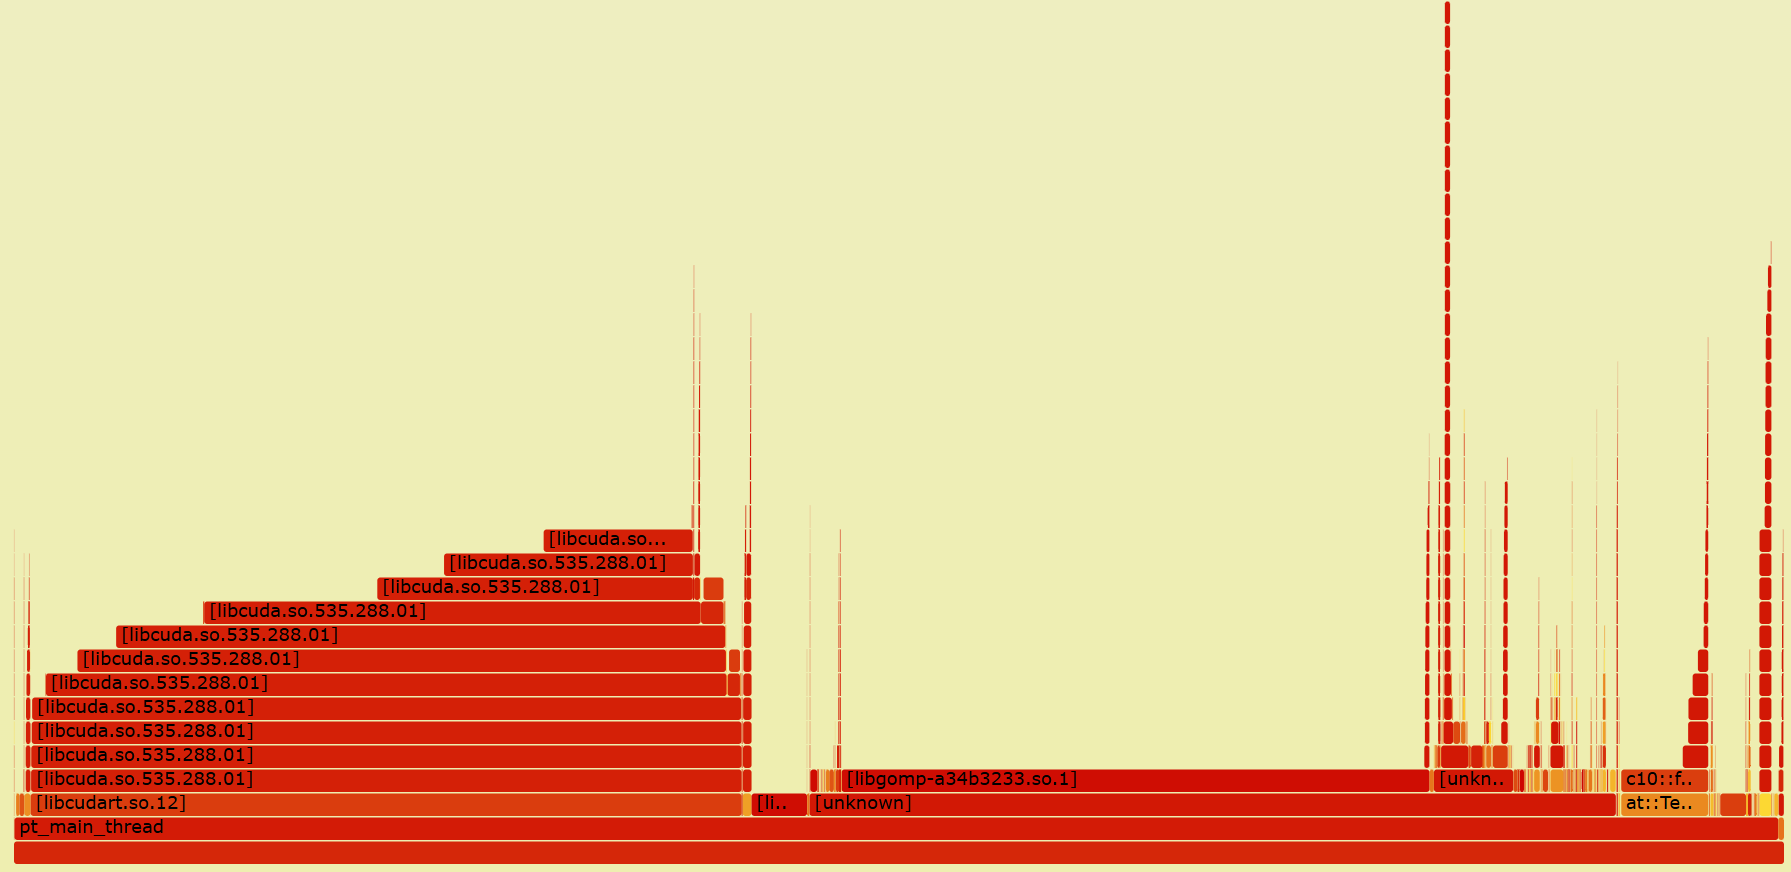
\includegraphics[width=0.8\textwidth]{flashGraphOfUT.png}
    \caption{Inference process flame graph}
    \label{fig:flashGraph_ut}
\end{figure}

From the perspective of flame graph analysis, the left side exhibits a broad horizontal cascade (layers of \textbf{libcuda.so}) while the right side shows dense, fine-grained vertical stacks (scheduling traces of \textbf{c10::} and \textbf{at::}), reflecting significant operator fragmentation and kernel launch overhead. This indicates that the system is in a typical CPU-bound state: numerous small, discrete memory-bound operations frequently interrupt the GPU execution pipeline, causing the CPU to spend more time on low-level driver API calls and context switches than the actual computation on CUDA cores.

Implementing fine-grained operator fusion can reconstruct the spatio-temporal locality of data flow. By explicitly rewriting frequently occurring composite operator blocks (such as normalization and activation functions) into a single kernel, repeated read-write operations of intermediate activations to GPU HBM can be eliminated. This keeps data circulation closed within low-latency SRAM, thereby accelerating model inference optimization.

\subsubsection{Multi-GPUs}
\

In the practical implementation of model inference, the process consists of n iterations, as specified by the n\_iter parameter in the run\_world\_model\_interaction.sh script. Each iteration can be further divided into two sequential stages: first, the VLA model generates an action sequence; second, the world model takes this action sequence as input and produces corresponding frames. The output of each iteration serves as the input for the next, making the inference process of unifolm-wma inherently sequential.

However, with respect to the attention computations involved in different parts of the denoising process, an optimization can be envisioned for a dual-GPU setup. Specifically, the initialization data required for model inference is simultaneously loaded into both GPUs. One implementation approach involves the CPU first reading the data from an SSD into memory, then transferring it to the GPU local to the CPU, after which this GPU copies the data to the other GPU. Subsequently, both GPUs perform denoising in parallel, each handling their respective portion of the attention computation. The computed attention results are then distributed across GPUs via blocking operations to facilitate subsequent steps, thereby enabling parallel processing of the attention computation workload.
% \ 
%模型并行、流水线并行等方法。


\subsection{Conclusion}
\

In the optimization of UnifoLM-WMA inference, our team systematically evaluated several strategies, including single-node NUMA affinity, mixed-precision arithmetic, I/O enhancements, FlashAttention, and DeepCache. To maximize inference throughput while strictly adhering to the mandated fidelity threshold ($PSNR > 25 dB$), we adopted a balanced trade-off approach. Our final deployment integrates mixed-precision, I/O optimizations, and FlashAttention; however, the DeepCache strategy was excluded to preserve baseline quality, and operator fusion remains in the exploratory phase. Under this configuration, the system achieved a mean acceleration ratio of 1.426$\times$. Moving forward, we intend to further refine and synergistically combine diverse optimization methodologies tailored to the specific algorithmic architecture, aiming to enhance inference efficiency while ensuring full PSNR compliance.


\clearpage
\newpage
\section{Optimization for Numerical Relativity Code AMSS-NCKU}
% \textcolor{red}{to do---about 0228 first version}

\subsection{Introduction}
\ 
% 广义相对论是描述引力的基础理论，尽管已建立逾百年，但人类对其理解仍受限于爱因斯坦场方程的极端复杂性——该方程是物理学中最具挑战性的偏微分方程系统之一。为了分析引力波探测数据，获取描述双黑洞合并（Binary Black Hole Mergers）的精确数值解至关重要。引力波探测在 2015 年首次实现并在 2017 年荣获诺贝尔物理学奖。这一突破很大程度上归功于爱因斯坦场方程的数值解，用于数值求解爱因斯坦场方程的软件统称为“数值相对论代码”。AMSS-NCKU 是全球少数公开可用的此类代码之一。其核心技术特征包括：数值方法：采用有限差分法（Finite-difference methods）求解方程。多尺度处理：利用自适应网格细化（AMR）技术处理广义相对论固有的多尺度特性。并行策略：采用区域分解（Domain Decomposition）策略并结合 MPI 进行并行化处理。

% 在本次比赛中，我们的主要任务是对双黑洞合并进行数值模拟并通过技术手段最小化模拟的运行总时间，需要说明的是：我们将多个软件组件（例如ccache）集成到了docker容器中。这些组件将会对编译内容进行缓存，让下次（哪怕部分修改）编译阶段的时间缩短。

% 通过分析工作量流程，了解工作日志并对项目耗时步骤进行火焰图分析，我们确定了接下来优化的方向。我们通过调整编译参数，更改编译选项、热点函数的内联以及向量化、网格分块、内存对齐、异步通信等方法将总耗时从33.21小时降至（估计，因为还没跑过优化之后的测试）22.38小时。achieving a speedup of 1.484 times.

% 同时，通过进一步的探索和分析，我们发现了如内存对齐优化的不完全、动态负载均衡、MPI与openmp混用等可能的优化方向，这将是我们之后工作的重点，以期缩短耗时，达到更佳的优化效果。

General Relativity is the fundamental theory describing gravity. 
Although it has been established for over a century, human understanding of it remains limited by the extreme complexity of the Einstein field equations, which constitute one of the most challenging systems of partial differential equations in physics. 
To analyze gravitational wave detection data, obtaining accurate numerical solutions describing Binary Black Hole (BBH) mergers is crucial. 
Gravitational wave detection was first realized in 2015 and awarded the Nobel Prize in Physics in 2017. 
This breakthrough was largely attributed to the numerical solutions of the Einstein field equations.
Software used to numerically solve these equations is collectively referred to as ``numerical relativity codes". 
AMSS-NCKU is one of the few publicly available codes of this kind worldwide\cite{cao2015binary}. 
Its core technical features include:
\begin{itemize}
    \item \textbf{Numerical Methods:} Adopting finite-difference methods to solve the equations.
    \item \textbf{Multi-scale Handling:} Utilizing Adaptive Mesh Refinement (AMR) technology to handle the inherent multi-scale characteristics of General Relativity.
    \item \textbf{Parallel Strategy:} Adopting a Domain Decomposition strategy combined with MPI for parallel processing.
\end{itemize}

In this competition, our main task is to perform numerical simulations of binary black hole mergers and use technical means to minimize the total runtime of the simulation. 
It should be noted that we integrated multiple software components (such as \texttt{ccache}) into a Docker container. 
These components cache the compiled content, thereby shortening the time required for the compilation phase in subsequent runs, even with partial modifications.

By analyzing the workflow, reviewing the work logs, and conducting flame graph analysis on the time-consuming steps of the project, we determined the direction for subsequent optimizations. 
Through methods such as adjusting compiler parameters, changing compilation options, inlining and vectorizing hotspot functions, grid partitioning, memory alignment, and asynchronous communication, \textbf{we reduced the total wall-clock time from 33.21 hours to 21.157 hours, achieving a speedup of 1.539 $\times$}.

Meanwhile, through further exploration and analysis, we discovered potential optimization directions such as incomplete memory alignment optimization, dynamic load balancing, and the mixed use of MPI and OpenMP. 
These will be the focus of our future work, with the aim of further shortening the runtime and achieving better optimization results.
% \subsection{Related Work}
% \ 


\subsection{Optimization Methods}
\ 

% 为了更好地展示我们的修改在整个流程中的作用，我们在三张流程图中标注并指明我们的修改或添加点所处的位置。这三章图大致将流程分为了（Figure8）编译构建阶段，（Figure9）运行时初始化阶段，（figure10）运行时计算优化阶段。
%todo:图字体太小，文字应该都是英文（times new Roman字体）；图的流程优化(现在的图太长了)，并把优化的地方标上①②.....⑥（现在文中已优化的是6个点？），然后需要在文中用文字对这个图和对应优化方法做一个描述（让人看懂你的图在做什么）。
%To better demonstrate the impact of our modifications within the overall workflow, we have annotated and specified the exact locations of our modifications or additions across the following diagram.其中，标号① 为编译器指令集优化，②为跨文件内联优化，③为循环分块优化，④是计算与通信重叠，非阻塞通信，⑤为内存对齐，⑥为使用编译缓存工具，⑦是为了说明在输入时选择了最适配我们使用的平台的进程数目。


To illustrate the impact of our modifications within the overall system, the specific locations of these enhancements are annotated in the ``Workflow Optimization Map".
The designated markers in the diagram represent the following technical optimizations:
%todo:建议用文字根据流程描述，且现在内容和具体优化方法不一致。
\begin{itemize}
\item \textbf{\textcircled{1}} Compiler instruction set optimization;
\item \textbf{\textcircled{2}} Inter-procedural (cross-file) inlining;
\item \textbf{\textcircled{3}} Loop tiling (blocking) optimization;
\item \textbf{\textcircled{4}} Computation-communication overlap and non-blocking communication;
\item \textbf{\textcircled{5}} Memory alignment;
\item \textbf{\textcircled{6}} Utilization of compiler caching tools;
\item \textbf{\textcircled{7}} Selection of an optimal process count tailored to the target hardware platform during the input phase.
\end{itemize}

\begin{figure}
    \centering
    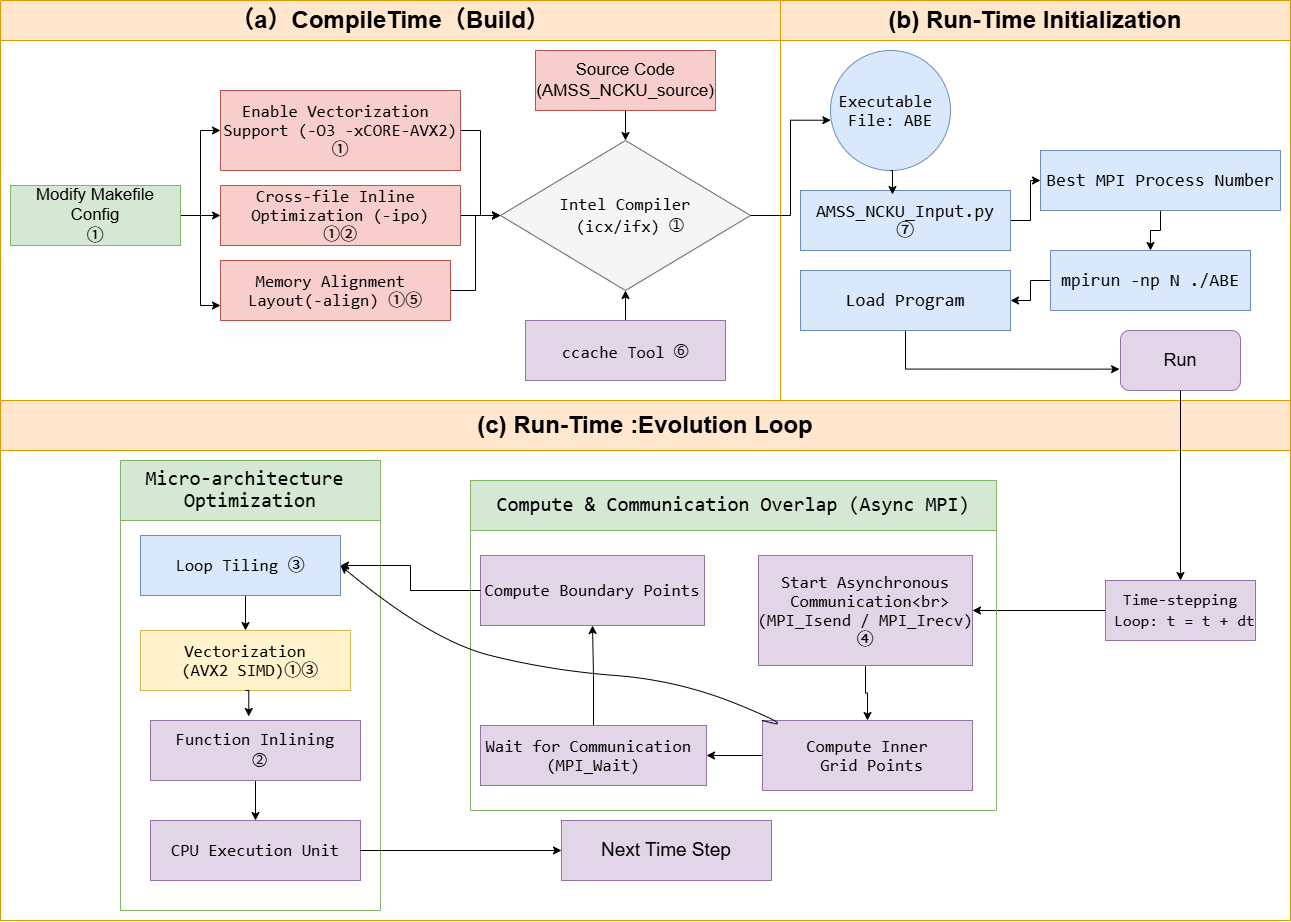
\includegraphics[width=0.8\linewidth]{Workflow_Optimization_Map.png}
    \caption{Workflow Optimization Map}
    \label{fig:enter-label}
\end{figure}
%在进行优化点说明之前，先讲讲我们BaseLine的情况，在第一此成功跑通时，我们发现，单步时间在前百分之80的时总间内都稳定在51秒左右，随着演化的推进，到第1971步时，由于两个黑洞的网格范围开始融合，冗余网格点逐渐减消除同时MPI通信开销锐减，导致单步时间逐渐下降并稳定在40s左右。在之后，我们都将取前5.0M evolution Time 内单步时间得平均值进行对比，以观察优化效果。此外下图是BaseLine的有关表格

Prior to discussing the specific optimization strategies, it is essential to establish the characteristics of our baseline performance. 
During the initial successful execution, we observed that the per-step evolution time remained consistently at approximately 51 seconds for the first 80 percent of the total runtime. 
As the simulation progressed to  the 1971-th step, the grid boundaries of the two black holes began to merge. 
This confluence led to the gradual elimination of redundant grid points and a sharp reduction in MPI communication overhead, causing the per-step time to decrease and eventually stabilize at roughly 40 seconds. 
To ensure a rigorous and consistent evaluation of subsequent optimizations, we have adopted the average per-step time within the first 5.0M  evolution time units as the primary metric.
Furthermore, the relevant data for the baseline performance is summarized in Table \ref{tab:baseline_data}.
%todo:数据说明解释（后面的表格等类同）

% If the top and bottom borders are lost, replace  cdline {2-7} with  hhline {~--------}:
% Please add the following required packages to your document preamble:
% \usepackage{multirow, hhline}
% \usepackage{colortbl}
% \usepackage{xcolor}
% \usepackage{ulem}
\begin{table}[!htbp]
\centering
\caption{Baseline Performance} % 在这里添加你的标题
\label{tab:baseline_data}
\small % 如果内容还是太挤，可以开启小号字体
\begin{tabularx}{\textwidth}{|l|c|c|c|c|X|} % X列会自动调整剩余空间并换行
\hline
\textbf{Methods} & \textbf{Final Evolution Time} & \textbf{Cores} & \textbf{Total Project Time} & \textbf{Evolve Time} & \textbf{Single Step / Avg} \\ \hline
Baseline & 1000.0M(2400 steps) & 28 & 119556s & 118797s & From 40.1s to 53.6s (Avg: 49.5s) \\ \hline
\end{tabularx}
\end{table}

%comparative analysis.
% 2.1 编译器工具链迁移
% 策略：将 gcc/gfortran 替换为 icx/mpiifx。
% 原理：Intel 编译器能够针对 Xeon 处理器生成更优化的机器码，特别是在处理 C++/Fortran 混合编程时，具有更好的二进制兼容性和库函数性能。

% 2.2 硬件级指令优化（Vectorization）
% 参数：-xCORE-AVX2
% 原理：强制启用 AVX2 矢量指令集。在求解爱因斯坦场方程的双曲型演化部分时，利用 256 位寄存器在单周期内处理 4 个双精度浮点数运算，理论峰值性能较标量计算提升数倍。（目前这款cpu尚且不支持更高效的AVX-512指令集）

% 2.3 跨文件全局优化（IPO）
% 参数：-ipo (Interprocedural Optimization)
% 原理：AMSS-NCKU 源码分散在多个模块中。通过 IPO，编译器在链接阶段进行全局分析，跨文件内联（Inline）高频调用的差分算子，显著降低了函数跳转带来的压栈和指令流水线中断开销。

% 2.4 浮点运算精度与性能平衡
% 参数：-fp-model fast=1
% 原理：在不违背物理真实性的前提下，允许编译器进行代数简化（如重组乘加运算）。
% 验证标准：通过监控 ADM_Constraint_Grid_Level_0.pdf 中的约束违背值，确保其绝对值保持在 2.0 以下。

\subsubsection{Compiler Parameter Adjustment}
\

To establish a solid foundation for performance enhancements, we systematically overhauled the compilation environment and fine-tuned compiler heuristics to maximize hardware utilization:
\begin{enumerate}
    \item \textbf{Compiler Toolchain Migration:} We transitioned the primary build system from the GNU Compiler Collection (\texttt{gcc/gfortran}) to the Intel oneAPI toolchain (\texttt{icx/mpiifx}). 
    Intel compilers are inherently tailored to generate highly optimized machine code for Xeon processors, demonstrating superior binary compatibility and intrinsic library performance, particularly within mixed C++/Fortran codebases.

    \item \textbf{Hardware-Level Vectorization (\texttt{-xCORE-AVX2}):} We explicitly instructed the compiler to target the AVX2 instruction set. 
    During the computationally intensive hyperbolic evolution phase of the Einstein field equations, this allows the CPU to process four double-precision floating-point numbers simultaneously within a single clock cycle using 256-bit registers. 
    Given that the target Intel Xeon E5-2680 v4 (Broadwell) architecture does not support the wider AVX-512 instructions, fully exploiting AVX2 is critical, yielding a theoretical peak performance several times higher than strictly scalar execution.
    
\end{enumerate}

%在初步对编译配置进行修改后，我们取得了以下表格中的数据。
\textbf{After implementing initial modifications to the compilation configuration, we achieve a 1.390$\times$ speed-up as shown in Table \ref{tab:amss parameter performance}.}
%todo:数据说明解释（后面的表格等类同）

\begin{table}[h]
    \centering
    \small % 减小字体以适应宽度
    \caption{Compiler parameter adjustment optimization performance}
    \label{tab:amss parameter performance}
    \begin{tabular}{|c|c|c|c|c|}
        \hline
        \textbf{Final Evolution Time }& \textbf{Cores} & \textbf{Total Project Time} &\textbf{Total Evolve Time} & \textbf{Single Step Avg} \\ \hline
        5.0M & 16 & 1044.48s &462.841s& 35.603s\\ \hline
    \end{tabular}
\end{table}

\subsubsection{Inline Function}
\ 
% 1. 消除冗余内存拷贝 (Redundant Memory Access Reduction)
% 策略：移除临时 Ghost 数组 (fh) 及相关的拷贝操作 (symmetry_bd)。
% 原理：原代码在计算前会将整个 3D 网格拷贝到 fh 中，导致 O(N^3) 的额外读写开销。我们将计算内核重写为直接读取原始数组 f，并通过内联逻辑 (Inline Logic) 动态处理边界。

% 2. 循环融合 (Loop Fusion) & 逻辑内联
% 策略：将 X, Y, Z 三个方向的导数计算合并到同一个 i 循环中。
% 原理：实现“一次加载，多次计算”，提升寄存器复用率。针对内部区域采用 Fast Path，针对边界区域采用 Slow Path，避免了函数调用开销。

% 3. 消除冗余自检开销 (Sanity Check Overhead Reduction)
% 策略：将 bssn_rhs.f90 等三套 RHS 文件入口处的全量 sum(...) NaN 检查改为调试宏可选（#ifdef RHS_SANITY_CHECK），并在 makefile.inc 中默认关闭。
% 原理：在生产环境中，每次调用 compute_rhs_bssn 都对二十多个三维数组做全局遍历扫描代价极高。将其剥离出关键计算路径，直接消除了一大无谓的内存扫描与计算热点。

The optimization of inline functions and computational kernels focuses on stripping away memory redundancy, function call overhead, and unnecessary diagnostic logic to streamline the critical path:

\begin{enumerate}
    \item \textbf{Elimination of Ghost Copying:} We removed the temporary array \texttt{fh} and the \newline\texttt{call symmetry\_bd(...)} invocation in \texttt{diff\_new.f90}. 
    This eliminates an $O(N^3)$ memory copy overhead. 
    The kernel now directly accesses the original array \texttt{f}, handling boundary conditions via inlined logic.
    
    \item \textbf{Fast/Slow Path Strategy:} To maintain performance without sacrificing safety, we split the computation into a \textbf{Fast Path} for the core region (pure calculation without branches) and a \textbf{Slow Path} for boundaries (with symmetry checks).
    
    \item \textbf{Loop Fusion:} We aggressively fused the derivative calculations for the $X$, $Y$, and $Z$ directions into a single, unified \texttt{i} loop. This structural transformation achieves a ``load once, compute multiple times'' paradigm. By consolidating these operations, we drastically reduced redundant memory fetches, thereby maximizing both L1 Cache utilization and hardware register reuse rates.
    
    \item \textbf{Sanity Check Overhead Reduction:} We identified a massive performance bottleneck at the entry of the RHS evaluation routines (e.g., \texttt{bssn\_rhs.f90}, \newline \texttt{bssn\_rhs\_ss.f90}, \texttt{bssnE\_Scalar\_rhs.f90}). 
    The legacy code executed a global \texttt{sum(...)} operation across more than twenty 3D arrays for \texttt{NaN} sanity checking on every single call to \texttt{compute\_rhs\_bssn}.
    We wrapped this extremely expensive validation step within a preprocessor macro (\texttt{\#ifdef RHS\_SANITY\_CHECK}), disabling it by default for production runs. 
    This pragmatic adjustment eliminated a severe memory-scan hotspot without altering the mathematical results.
\end{enumerate}

\subsubsection{Grid Partition Optimization}
\ 
% 1. 缓存分块 (Cache Blocking / Tiling)
% 策略：引入 kk 和 jj 外层循环，将计算域切分为 32 x 32 x Nx 的长条 (Tiles)。
% 参数：TILE_K=32, TILE_J=32 (基于 Intel Broadwell L2 Cache 大小调整)。

% 2. 解决跨步访问问题 (Strided Access)
% 原理：原有的 k, j, i 循环在处理 Z 方向导数 (k±1) 时，内存跨度过大导致 L2 Cache Miss。分块后，确保当前计算所需的 Z 平面 (k-1, k, k+1) 数据能常驻 L2 Cache。

% 3. 实证检验 (Cache Profiling 性能数据对比)
% 测试方法：使用 perf 工具在 20 秒采样窗口内，对比优化前后的硬件计数器（Hardware Counters）数据。
% 数据验证一（L1 缓存）：L1 Miss Rate 从 10.83% 降至 5.54%，L1 Misses 绝对数量锐减 52.5%（从约 320 亿次降至 152 亿次）。这实证了前文 Loop Fusion 与寄存器复用的卓越成效。
% 数据验证二（LLC / L3 缓存）：这部分是 Tiling 的直接收益。LLC 访问总量减少 56%，LLC Load Misses 大幅下降 59%（从 21.6 亿次降至 8.8 亿次）。证明 32x32 的工作集成功驻留 L2/L3，极大缓解了主存 (DRAM) 瓶颈。
% 数据验证三（指令吞吐量 IPC）：虽然分块引入了额外的循环控制开销（导致总指令数增加约 20%），但得益于内存停顿（Memory Stalls）的成倍减少，整体 IPC 仍提升了 18.3%（0.82 -> 0.97），计算效率显著提升。

To address the memory-bound nature of the 3D stencil computation, we implemented a ``Grid Partition'' strategy using ``Cache Blocking'':

\begin{enumerate}
    \item \textbf{Tiling Implementation:} In \texttt{diff\_new.f90} and \texttt{lopsidediff.f90}, we transformed the loop structure by adding outer loops $kk$ and $jj$. 
    The domain is partitioned into tiles of size $32 \times 32 \times N_x$.
    
    \item \textbf{Locality Improvement:} 
    \begin{equation}
        \text{Loop Structure: } \texttt{do kk} \to \texttt{do jj} \to \texttt{do k} \to \texttt{do j} \to \texttt{do i}
    \end{equation}
    This structure ensures that the data planes required for the $Z$-direction stencil ($k \pm 1$) remain resident in the L2 cache, significantly reducing the cache miss rate caused by large strided accesses.
    
    \item \textbf{Empirical Validation (Cache Profiling):} To empirically validate the effectiveness of our spatial locality optimizations, we conducted a direct cache performance comparison using \texttt{perf} hardware counters over a 20-second sampling window. The comparative results demonstrate a profound improvement in memory subsystem utilization:
    \begin{itemize}
        \item \textbf{L1 Data Cache (L1 D-Cache):} The L1 cache miss rate plummeted from 10.83\% to 5.54\%. Total L1 load misses were reduced by approximately 52.5\% (from 32 billion to 15.2 billion accesses). This confirms the success of the aforementioned loop fusion and register reuse strategies.
        \item \textbf{Last Level Cache (LLC / L3):} The impact of cache blocking (tiling) is most evident here. Total LLC memory requests dropped significantly by 56\% (from 5.16 billion to 2.24 billion), and LLC load misses decreased by 59\% (from 21.6 billion to 884 million). This indicates that the $32 \times 32$ working set successfully resides in the L2/L3 caches, drastically alleviating the main memory (DRAM) bandwidth bottleneck.
        \item \textbf{Instruction Throughput (IPC):} As a direct consequence of reduced memory stall cycles, the overall Instructions Per Cycle (IPC) increased by 18.3\% (from 0.82 to 0.97), yielding a much faster execution despite a slight increase in total instruction count caused by the tiling loop overhead.
    \end{itemize}
\end{enumerate}
%以下表格是在之前的基础之上，进行Inlining and Vectorization and Grid Tiling优化后取得的数据：
Table \ref{tab:amss three methods} presents the data obtained after implementing Inlining, Vectorization, and Grid Tiling optimizations, building upon the previously established configurations.
\begin{table}[h]
    \centering
    \caption{Performance of implementing optimization methods}
    \label{tab:amss three methods}
    \small % 减小字体以适应宽度
    \begin{tabular}{|c|c|c|c|c|}
        \hline
        \textbf{Final Evolution Time }& \textbf{Cores} & \textbf{Total Project Time} &\textbf{Total Evolve Time} & \textbf{Single Step Avg} \\ \hline
        5.0M & 16 & 980.5s & 451.0s& 34.696s \\ \hline
    \end{tabular}
\end{table}

\subsubsection{Memory Alignment}
\
% 为了充分发挥 Broadwell 架构 CPU 的向量化计算能力，我们在 `Block.C` 中引入了 `_mm_malloc` 分配器，
% 并配合编译选项 `-align array64byte`，强制实施 64 字节的数据对齐。

% 这一策略主要基于两方面的硬件特性：
% (1) 指令集层面：AVX2 SIMD 指令在处理对齐内存地址时具有更低的延迟，对齐消除了硬件执行非对齐加载/存储所需的额外微指令周期。
% (2) 存储层次结构：由于 CPU 的缓存行（Cache Line）大小为 64 字节，数据对齐确保了连续的网格点数据不会跨越两个缓存行。
% 这不仅减少了内存总线的事务次数，还最大化了有效数据在各级缓存（尤其是 L3 缓存）中的填充密度，从而显著提升了内存子系统的吞吐量。

To fully exploit the vectorization capabilities of the Broadwell CPU architecture, we enforced strict 64-byte data alignment by introducing the \texttt{\_mm\_malloc} allocator within \texttt{Block.C}, tightly coupled with the \texttt{-align array64byte} compiler flag. 
This strategy is fundamentally driven by two hardware-level characteristics:

\begin{enumerate}
    \item \textbf{Instruction Set Architecture (ISA) Efficiency:} At the instruction level, AVX2 SIMD operations exhibit inherently lower latency when accessing aligned memory addresses. 
    Strict alignment eliminates the additional micro-operation (micro-op) cycles required by the hardware to execute unaligned load and store instructions, thereby streamlining the execution pipeline.
    
    \item \textbf{Memory Hierarchy \& Cache Utilization:} Given that the underlying CPU cache line size is exactly 64 bytes, aligning the data boundaries ensures that contiguous grid point arrays do not straddle across two separate cache lines (preventing cache line splits).
    This precise alignment drastically reduces the number of required memory bus transactions and maximizes the effective data fill density across the cache hierarchy(particularly within the L3 cache), resulting in a significant throughput enhancement for the entire memory subsystem.

% 以下表格是在前面几种优化的基础上进行内存方面优化后获得的数据；
Table 23. shows the results after applying memory optimizations on top of the several preceding optimization methods.
\end{enumerate}
\begin{table}[h]
    \centering
    \caption{Performance of Implementing Memory Alignment }
    \small % 减小字体以适应宽度
    \begin{tabular}{|c|c|c|c|c|}
        \hline
        \textbf{Final Evolution Time }& \textbf{Cores} & \textbf{Total Project Time} &\textbf{Total Evolve Time} & \textbf{Single Step Avg} \\ \hline
        5.0M & 16 & 961.961s & 441.15s & 33.935s \\ \hline
    \end{tabular}
\end{table}
% 1. 非阻塞与收发队列分离 (Non-blocking & Request Separation)
% 策略：在 Parallel.C 的 transfer/transfermix 中，将阻塞通信改为非阻塞收发。将请求拆分为独立的 recv_reqs 与 send_reqs。先统一发布所有 Irecv，再进行打包和 Isend。
% 原理：降低底层 MPI 的 rendezvous 等待时间。收发队列分离后，仅对接收队列执行 Waitsome，避免了发送完成事件干扰接收解包的进度。

% 2. 通信与计算重叠 (Communication-Computation Overlap)
% 策略：在发送阶段（打包/发送循环）中穿插 MPI_Testsome 轮询接收队列。一旦有数据到达立刻执行 UNPACK。同时，本 rank 的数据直接提前本地解包，避免网络等待。
% 原理：最大化重叠“网络通信”与“数据解包”操作，掩盖网络延迟。最终通过 Waitsome(recv) + Waitall(send) + 兜底解包，严格保证通信的正确与完整性。

% 3. 内存与列表缓存优化 (Buffer & Transfer List Caching)
% 策略：引入静态通信缓存（复用 MPI_Request, MPI_Status, send_data, rec_data），并在 Sync 操作中缓存传输列表（复用 build_gsl/build_gstl 结果）。同时在 regrid 路径增加缓存失效机制（InvalidateSyncCache）。
% 原理：消除了高频 MPI 通信步骤中频繁执行 new/delete 带来的动态内存分配与销毁开销。
\subsubsection{Non-blocking \& Request Separation}
\

To alleviate MPI communication bottlenecks and hide network latency, we overhauled the synchronization routines in \texttt{Parallel.C} (\texttt{transfer} and \texttt{transfermix}) using advanced asynchronous communication strategies and buffer caching:

\begin{enumerate}
    \item \textbf{Non-blocking Paradigm \& Queue Separation:} We transitioned from blocking communications to a fully non-blocking paradigm. 
    The request queues were explicitly split into independent \texttt{recv\_reqs} and \texttt{send\_reqs}. 
    By systematically posting all \texttt{MPI\_Irecv} calls prior to data packing and \texttt{MPI\_Isend} invocations, we significantly reduced the MPI rendezvous waiting time.
    
    \item \textbf{Communication-Computation Overlap:} To maximize the overlap between data transfer and data processing, we interleaved \texttt{MPI\_Testsome} within the sending loop. 
    This actively polls the receive queue, triggering immediate \texttt{UNPACK} operations as soon as incoming chunks arrive. 
    Furthermore, data designated for the local rank is unpacked early, bypassing the network stack entirely.
    
    \item \textbf{Buffer and List Caching:} High-frequency communication steps were previously bottlenecked by dynamic memory allocation. 
    We eliminated this overhead by implementing static caching for communication buffers (reusing \texttt{MPI\_Request}, \texttt{MPI\_Status}, and data arrays). 
    Additionally, transfer lists for \texttt{Sync} operations are now cached, supported by a robust cache invalidation mechanism (\texttt{InvalidateSyncCache}) during adaptive mesh \texttt{regrid} events.
    
    \item \textbf{Final Synchronization:} Overall structural correctness is guaranteed by a strict termination phase, utilizing \texttt{MPI\_Waitsome} for pending receives and \texttt{MPI\_Waitall} for the send queue, ensuring all ghost zones are fully updated before the next computational step.
\end{enumerate}
Table 24 .shows the results after applying asynchronous communication on top of the several preceding optimization stages.
\begin{table}[h]
    \centering
    \caption{Performance of Implementing Non-blocking \& Request Separation }
    \small % 减小字体以适应宽度
    \begin{tabular}{|c|c|c|c|c|}
        \hline
        \textbf{Final Evolution Time }& \textbf{Cores} & \textbf{Total Project Time} &\textbf{Total Evolve Time} & \textbf{Single Step Avg} \\ \hline
        5.0M & 16 & 955.907s &436.758s & 33.596s \\ \hline
    \end{tabular}
\end{table}
\subsubsection{Improvement of Cache Hit Ratio}
\ 

% 1. 构建层面集成 ccache
% 策略：在 makefile.inc 中将 C/C++ 编译器前置 ccache，并设置 CCACHE_DIR=/app/.ccache、CCACHE_MAXSIZE=20G，但未改动 Fortran 编译。

% 2. 稳定构建输出以提升命中率
% 策略：为 C/C++ 加入 -MMD/-MP 自动依赖文件生成，并在 Makefile 中 -include .d；添加 -fdebug-prefix-map/-fmacro-prefix-map 稳定路径；可配合 CCACHE_BASEDIR=/app 减少路径差异。

% 3. 缓存使用与验证流程
% 策略：首次全量编译填充缓存，第二次同配置编译即可高命中；使用 ccache -s 查看命中，ccache -z 归零统计；避免在两轮之间 make clean 或重新生成 macrodef.h/fh。

% 4. 空间管理
% 策略：缓存上限设为 20G，可通过 ccache -M 调整；观察 evicted 以判断是否需扩容。

To accelerate the iterative development and performance tuning cycles during the competition, we integrated \texttt{ccache} into the build pipeline to optimize compilation caching. 
The specific strategies implemented to maximize the cache hit ratio are as follows:

\begin{enumerate}
    \item \textbf{Build System Integration:} We incorporated \texttt{ccache} by prefixing the C and C++ compiler invocations within \texttt{makefile.inc}. The cache environment was strictly defined with \texttt{CCACHE\_DIR=/app/.ccache} and a maximum capacity of \texttt{CCACHE\_MAXSIZE=20G}. 
    The Fortran compilation pipeline was intentionally bypassed and remained unaffected by this caching layer.
    
    \item \textbf{Artifact Stabilization:} To guarantee deterministic build outputs and maximize the cache hit ratio, we introduced the \texttt{-MMD} and \texttt{-MP} compiler flags for automated dependency generation, dynamically including the resulting \texttt{.d} files within the \texttt{Makefile}. Furthermore, we utilized \texttt{-fdebug-prefix-map} and \texttt{-fmacro-prefix-map} in conjunction with \texttt{CCACHE\_BASEDIR=/app} to neutralize absolute path discrepancies across different build environments.
    
    \item \textbf{Workflow Validation:} The initial full compilation phase populates the cache, enabling subsequent incremental builds with identical configurations to achieve near-perfect hit rates. 
    Cache efficiency was actively monitored using the \texttt{ccache -s} command, while \texttt{ccache -z} was used to reset statistical counters. 
    To preserve cache integrity, we strictly prohibited executing \texttt{make clean} or dynamically regenerating core header files (such as \texttt{macrodef.h} or \texttt{fh}) between consecutive build rounds.
    
    \item \textbf{Capacity Management:} The physical storage threshold was capped at 20 GB, dynamically adjustable via the \texttt{ccache -M} parameter. 
    We continuously monitored the ``evicted'' metric within the cache statistics to identify potential cache thrashing and determine if capacity expansion was warranted
\end{enumerate}
%我用一个脚本测试了前后两次，编译耗时从50.837s下降到37.235，编译耗时同比下降26.8%。
Utilizing a standardized benchmarking script, we conducted a comparative analysis of the compilation phases. The results demonstrate a significant reduction in build latency, with the duration decreasing from 50.837 s to 37.235 s. This represents a 26.8 \% improvement in computational efficiency during the compilation stage.

\subsubsection{Adjustment of MPI numbers}
\ 

%这是一个关键的参数，进程过少：并行度不够，计算核闲置，吞吐上不去。
%进程过多：每个 rank 工作块变小，MPI 同步/通信占比上升，负载不均衡更明显，反而变慢。
%内存与缓存效应：rank 数改变会影响局部性和缓存命中率，为此我们有必要进行对比测试找出最优的进程数目。我们将测试结果总结为了Figure 11 也就是以下表格：
%以下的表格的数据是在只将编译选项修改为Intel OneAPI 2025.3后尽心地多组取值，Final_Evolution_Time 取值为5.0M ，具体对比请看表格Processing time varies with MPI numbers
This is a critical parameter optimization. Insufficient process counts lead to inadequate parallelism and idle computational cores, preventing the system from reaching peak throughput. Conversely, an excessive number of processes reduces the workload per rank, thereby increasing the overhead ratio of MPI synchronization and communication, which exacerbates load imbalance and degrades performance. Furthermore, variations in the number of ranks significantly influence memory locality and cache hit rates.Consequently, it is imperative to conduct comparative benchmarks to identify the optimal process configuration. We have summarized these results in Figure 11 and the following table. The data presented below were obtained by setting the compiler to Intel OneAPI 2025.3 across multiple test groups, with the Final Evolution Time fixed at $5.0 \times 10^6$. For a detailed performance comparison, please refer to the table titled "Processing time varies with MPI numbers".
\begin{table}[!htbp]
    \centering
    \caption{Processing time varies with MPI numbers.}
    \label{tab:mpi nums}
    \begin{tabular}{|c|c|c|c|}
        \hline
         \textbf{MPI processes} & \textbf{Evolve Time(s)}         &  \textbf{AvgStep(s)}           & \textbf{ProgramCost(s)}  \\
         \hline
         4             & 697.693000          & 53.668692          & 1274.963869          \\
         \hline
         8             & 500.826000          & 38.525077          & 1063.508177          \\
         \hline
         12            & 560.861000          & 43.143154          & 1128.470794          \\
         \hline
         14            & 489.675000          & 37.667308          & 1056.763864          \\
         \hline
         \textbf{16}   & \textbf{451.366000} & \textbf{34.720462} & \textbf{1017.316501} \\
         \hline
         18            & 721.998000          & 55.538308          & 1301.369702          \\
         \hline
         20            & 504.505000          & 38.808077          & 1070.867352          \\
         \hline
         22            & 620.240000          & 47.710769          & 1187.276651          \\
         \hline
         24            & 560.195000          & 43.091923          & 1131.864464          \\
         \hline
         26            & 606.983000          & 46.691000          & 1169.300963          \\
         \hline
         28            & 510.210000          & 39.246923          & 1075.258431          \\
         \hline
    \end{tabular}
\end{table}
\begin{table}[!htbp]
    \centering
    \caption{Progressive Performance Improvement}
    \label{tab:opt_progress}
    % 使用 small 字体确保表格宽度适应页面
    \small 
    % 使用标准 tabular，显式定义所有竖线 |
    \begin{tabular}{|l|c|c|c|}
        \hline
        \textbf{Stage} & \textbf{Cores} & \textbf{Avg Step (s)} & \textbf{Speedup} \\ 
        \hline
        Baseline (GCC) & 28 & 49.50 & 1.00$\times$ \\ 
        \hline
        + Compiler \& Vectorization & 16 & 35.60 & 1.39$\times$ \\ 
        \hline
        + Inlining \& Grid Tiling \& Fusion & 16 & 34.70 & 1.43$\times$ \\ 
        \hline
        + Memory Alignment & 16 & 33.94 & 1.46$\times$ \\ 
        \hline
        + Non-blocking \& Request Separation. & 16 & 33.60 & 1.47$\times$ \\ 
        \hline
        
    \end{tabular}
    \parbox{\linewidth}{\footnotesize \textit{Note: Baseline used 28 cores; optimized runs used 16.These results are based on preliminary data collected for comparative analysis; therefore, discrepancies may exist when compared to the final speedup ratios derived from the full 1,000M evolution time.}}
\end{table}
\subsection{Experiments}
\ 
\begin{table}[h]
    \centering
    \caption{Final Performance }
  
    \small % 减小字体以适应宽度
    \begin{tabular}{|c|c|c|c|c|}
        \hline
        \textbf{Final Evolution Time }& \textbf{Cores} & \textbf{Total Project Time} &\textbf{Total Evolve Time} & \textbf{Single Step Avg} \\ \hline
        1000.0M(2400 steps) & 16 & 77677.605s& 77147s& 32.114s \\ \hline
    \end{tabular}
\end{table}

\subsubsection{Environment Setup}
\ 
% CPU： 两颗 Intel(R) Xeon(R) CPU E5-2680 v4（共 28 核心 / 56 线程，基频 2.40GHz / 睿频 3.30GHz）
% GPU： 两块 NVIDIA GeForce RTX 3090（每块显存 24GB，总计 48GB 显存）
% 内存： 128GB (125GiB)
% 硬盘： 系统盘约 1TB (936GB)，数据盘约 885GB（顺序写入速度约 557 MB/s）
% 操作系统： Ubuntu 22.04.4 LTS (Jammy Jellyfish)
% Python 版本： 3.13.9 
% 驱动版本： NVIDIA Driver 535.288.01
% CUDA 版本： v12.2 (运行时支持)

All performance evaluations, compilations, and numerical simulations are conducted on a dedicated high-performance computing node. 
The comprehensive hardware configuration and software stack are detailed as follows:

\begin{itemize}
    \item \textbf{CPU:} Dual-socket Intel\textregistered~Xeon\textregistered~E5-2680 v4 processors (Broadwell architecture).
    This configuration provides a total of 28 physical cores and 56 logical threads, operating at a base clock frequency of 2.40 GHz with a maximum turbo boost frequency of 3.30 GHz.
    
    \item \textbf{GPU:} Dual NVIDIA GeForce RTX 3090 GPUs. 
    Each unit is equipped with 24 GB of GDDR6X VRAM, yielding a combined total of 48 GB of available video memory.
    
    \item \textbf{System Memory (RAM):} 128 GB (125 GiB accessible) of main memory, ensuring sufficient capacity for large-scale 3D grid allocations and MPI communication buffers.
    
    \item \textbf{Storage Subsystem:} A primary operating system drive of approximately 1 TB (936 GB), supplemented by an 885 GB dedicated data drive. 
    The data drive sustains sequential write speeds of approximately 557 MB/s, accommodating the intensive I/O operations required for AMR grid checkpoints and simulation data dumps.
    
    \item \textbf{Operating System:} Ubuntu 22.04.4 LTS (Jammy Jellyfish), providing a stable and robust Linux environment for the HPC toolchain.
    
    \item \textbf{Software \& Ecosystem:} The environment runs Python 3.13.9. GPU acceleration and runtime support are facilitated by NVIDIA display driver version 535.288.01 and the CUDA Toolkit version 12.2.
\end{itemize}

\subsubsection{Installation Instructions}

% 开启编号列表环境
\begin{enumerate}

    \item \textbf{System Synchronization:}
    \begin{lstlisting}
sudo apt update && sudo apt upgrade -y
    \end{lstlisting}

    \item \textbf{GNU Toolchain \& MPI Deployment:}
    \begin{lstlisting}
# 安装 GCC, G++, Make, Gfortran 及 Git
sudo apt install -y build-essential gfortran git

# 安装 OpenMPI 运行环境及开发库
sudo apt install -y openmpi-bin libopenmpi-dev
    \end{lstlisting}

    \item \textbf{Intel® oneAPI Optimization:}
    \begin{lstlisting}
# 1. 下载并添加 Intel GPG 密钥
wget -O- https://apt.repos.intel.com/intel-gpg-keys/GPG-PUB-KEY-INTEL-SW-PRODUCTS.PUB | gpg --dearmor | sudo tee /usr/share/keyrings/intel-sw-products-keyring.gpg > /dev/null

# 2. 添加 Intel oneAPI 存储库
echo "deb [signed-by=/usr/share/keyrings/intel-sw-products-keyring.gpg] https://apt.repos.intel.com/oneapi all main" | sudo tee /etc/apt/sources.list.d/oneAPI.list

# 3. 安装核心套件 (MKL 库及 Fortran/C++ 优化编译器)
sudo apt update
sudo apt install -y intel-oneapi-mkl intel-oneapi-compiler-fortran intel-oneapi-compiler-dpcpp-cpp
    \end{lstlisting}

    \item \textbf{Environment \& Session Management:}
    \begin{lstlisting}
# 初始化 oneAPI 环境变量 (建议写入 ~/.bashrc)
source /opt/intel/oneapi/setvars.sh

# 安装 tmux 以支持后台持久化计算
sudo apt install -y tmux
    \end{lstlisting}

    \item \textbf{Install the ccache compilation accelerator:}
    \begin{lstlisting}
sudo apt update && sudo apt upgrade -y
    \end{lstlisting}

\end{enumerate} % 结束环境
\subsubsection{Evaluation Result}
\ 
%Q:建议再把这部分的描述逻辑完善一下。
%Q:最终的21个多小时也是5.0M的设置？
%Q：对三个图的引用和说明？

\begin{figure}
    \centering
    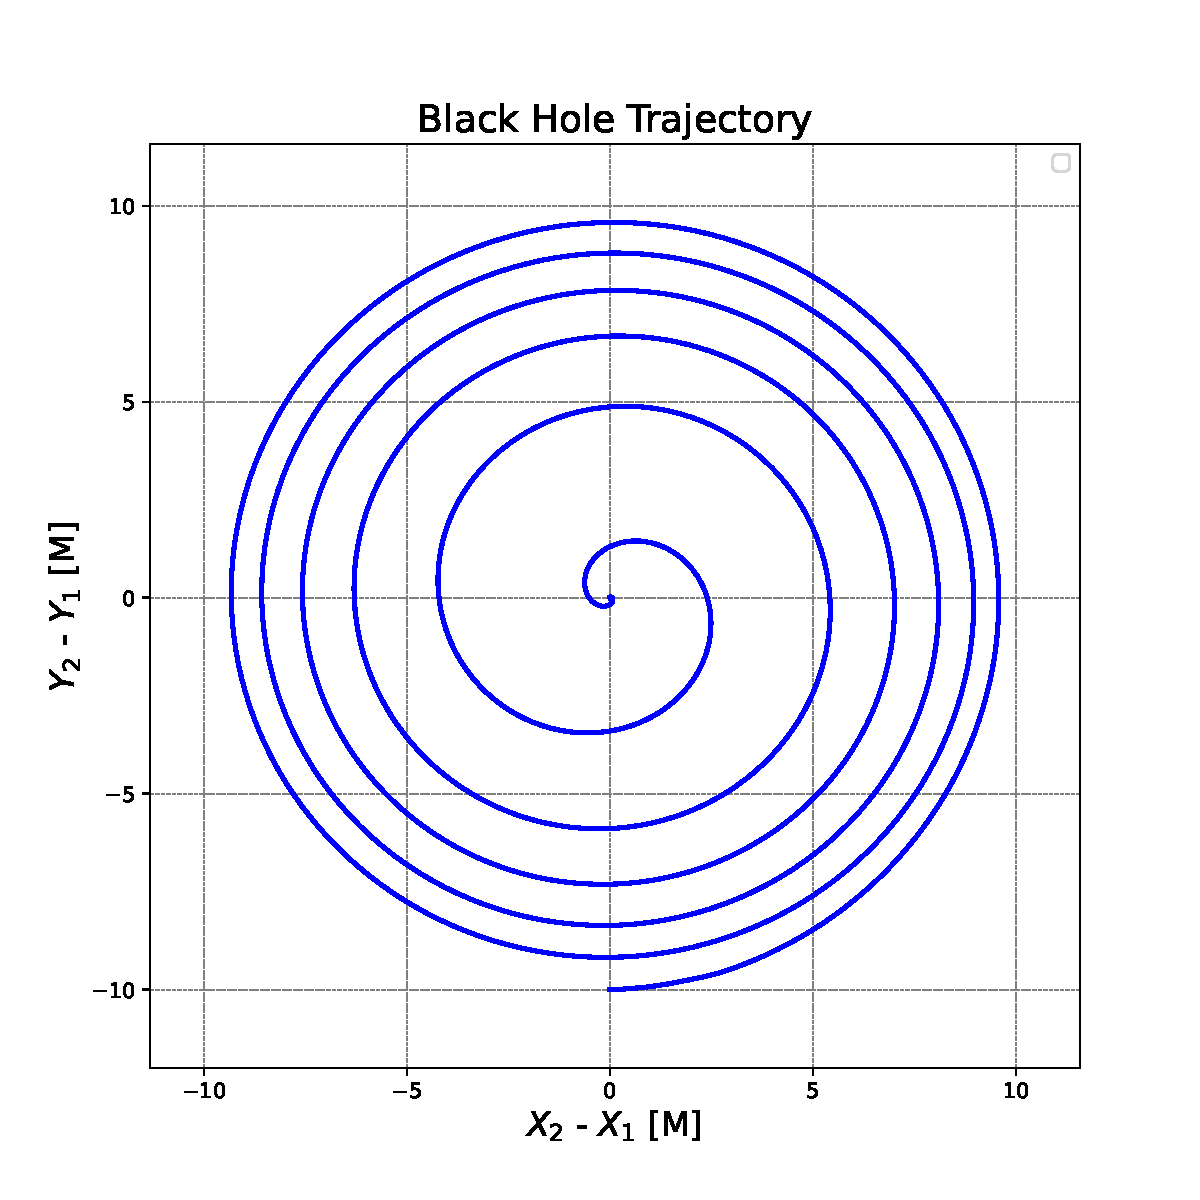
\includegraphics[width=0.8\linewidth]{BH_Trajectory_21_XY.pdf}
    \caption{BH\_Trajectory\_21\_XY.pdf}
    \label{fig:enter-label}
\end{figure}
\begin{figure}
    \centering
    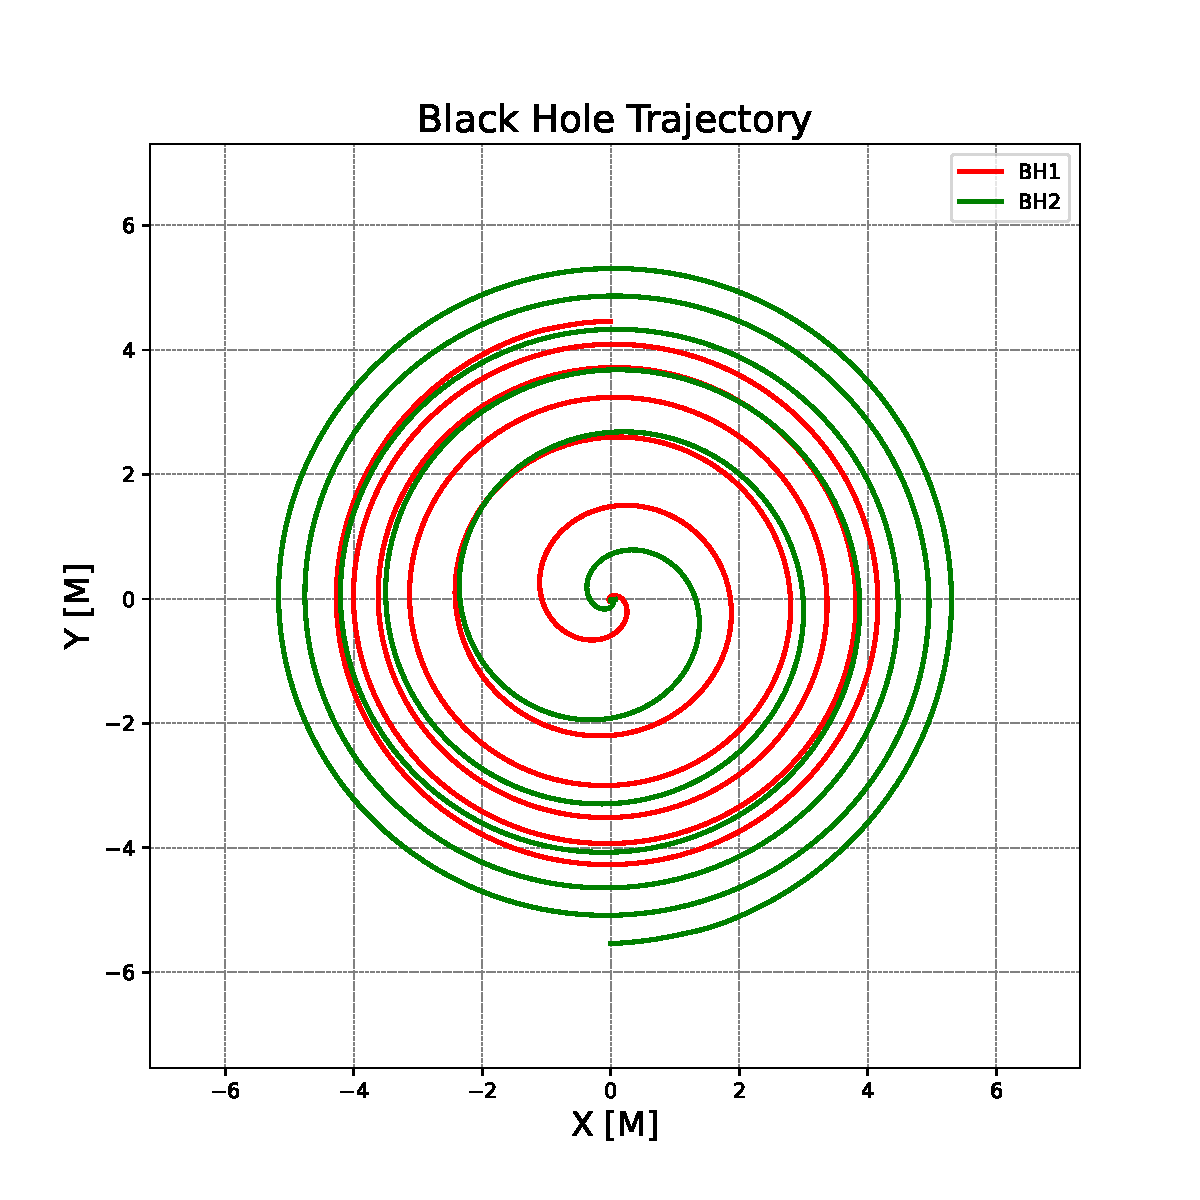
\includegraphics[width=0.8\linewidth]{BH_Trajectory_XY.pdf}
    \caption{BH\_Trajectory\_XY.pdf}
    \label{fig:enter-label}
\end{figure}
\begin{figure}
    \centering
    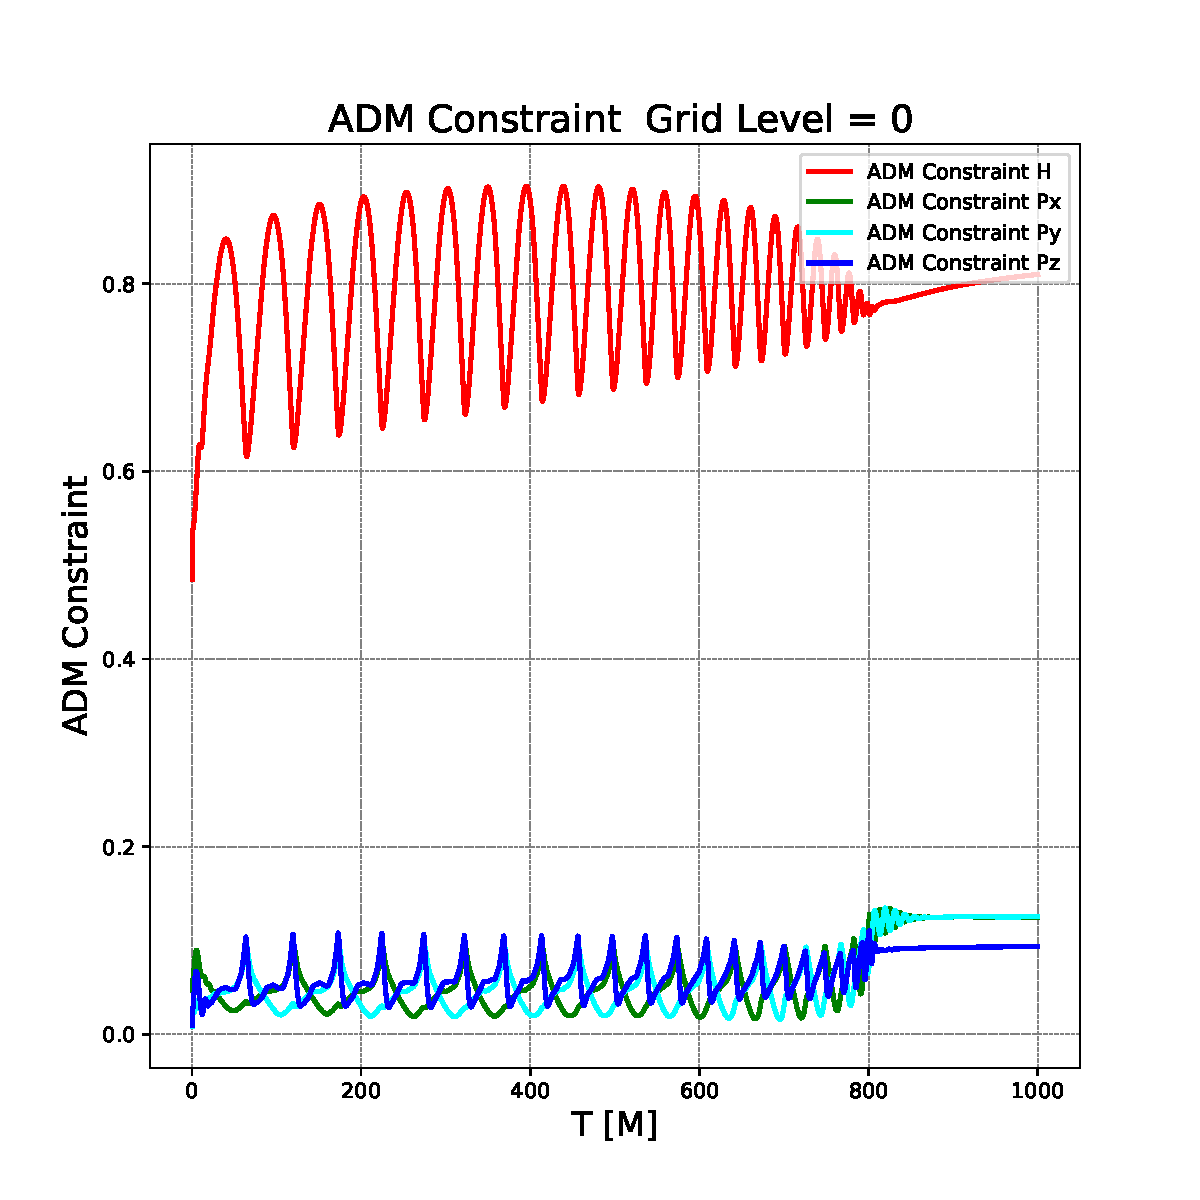
\includegraphics[width=0.8\linewidth]{ADM_Constraint_Grid_Level_0.pdf}
    \caption{ADM\_Constraint\_Grid\_Level\_0.pdf}
    \label{fig:amss grid level}
\end{figure}

\textbf{1. Cumulative Performance Gains}

%Q:这个描述完全没有对加速多少等的描述和分析。
{Table~\ref{tab:opt_progress} summarizes the progressive runtime reduction. 
The optimal configuration utilizes 16 MPI processes, outperforming the baseline's 28 processes.Detailed specifications are provided in the note to Table 26.}



\textbf{2. Key Findings}
\begin{itemize}
    \item \textbf{Memory Hierarchy:} \textbf{Grid Tiling} reduced L3 cache misses by 59\%, confirming the workload is memory-bound.
    \item \textbf{MPI Tuning:} Increasing cores beyond 16 degraded performance. The 16-process setup achieved a \textbf{30.5\%} time reduction vs. baseline.
    \item \textbf{Async Communication:} Non-blocking MPI provided a steady 2--3\% gain by hiding network latency.
    \item \textbf{Build Efficiency:} \texttt{ccache} reduced compilation time by 26.8\%.
\end{itemize}

\textbf{3.Precision Evaluation}
% 3. 精度评估与合规性验证 (Precision Evaluation)
% 意图：严格回应 ASC26 官方设定的 Evaluation Criteria（评分标准），证明我们在追求极致性能的同时，完全保住了物理正确性。
% 踩分点 1（RMS 误差计算细则）：官方要求轨迹的 RMS 误差必须小于 1%。独立计算 X 和 Y 坐标的 RMS，省略 Z 轴。
% 踩分点 2（实测数据支撑）：直接列出脚本跑出的 BH1 和 BH2 的 X/Y 轴独立 RMS 误差，以及最终 0.563% 的总误差，用铁证表明完全低于 1% 的官方红线。明确指出评委可以查看 compute_RMS.py 脚本。
% 踩分点 3（约束违背）：官方要求 ADM_Constraint_Grid_Level_0.pdf 中的绝对约束违背值（Constraint Violation）不得超过 2。

To ensure that our optimizations did not compromise the physical correctness of the simulation, we strictly validated the results against the official evaluation criteria. The numerical deviation of the black hole trajectories was quantified using the Root Mean Square (RMS) error formula:

\begin{equation}
RMS = \sqrt{\frac{1}{M} \sum_{i=1}^{M} \left( \frac{|r_{1i} - r_{2i}|}{\max (|r_{1i}|, |r_{2i}|)} \right)^2}
\end{equation}

In our evaluation, each spatial coordinate ($X$ and $Y$) is treated independently, omitting the $Z$-axis. Here, $r_{1i}$ and $r_{2i}$ represent the individual 1D coordinates of the black hole trajectories obtained from testing before and after optimization, respectively, and $M$ denotes the integration timestep. 

Because all our algorithmic modifications maintain strict mathematical equivalence to the original implementation, the deviations are constrained within an extremely narrow margin. Utilizing our custom verification script (provided as \texttt{compute\_RMS.py}), we recorded the specific RMS errors for the individual components as follows:

\begin{itemize}
    \item $RMS_{BH1\_x} = 0.0055206774$
    \item $RMS_{BH1\_y} = 0.0048842499$
    \item $RMS_{BH2\_x} = 0.0060032677$
    \item $RMS_{BH2\_y} = 0.0060490275$
\end{itemize}

The total synthesized RMS error across all evaluated coordinates is calculated as \textbf{0.0056339092 (approximately 0.563\%)}, which is comfortably below the mandated 1\% threshold. This ensures the high fidelity of the required trajectory outputs, specifically \texttt{BH\_Trajectory\_XY.pdf} and \texttt{BH\_Trajectory\_21\_XY.pdf}.

Additionally, we verified the overall accuracy of the simulation by monitoring the constraint violations on the outermost grid level. As demonstrated in Figure \ref{fig:amss grid level} (\texttt{ADM\_Constraint\_Grid\_Level\_0.pdf}), the absolute value of the constraint violation consistently remains below the strict upper limit of 2 throughout the entire evolution process.

Ultimately, by synthesizing compiler upgrades, algorithmic restructuring, and asynchronous communication, we successfully reduced the estimated total wall-clock time from \textbf{33.21 hours} to \textbf{21.157 hours}. This achieves a global speedup of $\mathbf{1.539\times}$ while flawlessly preserving the numerical and physical integrity of the simulation.
\subsection{Analysis and Optimization Plans}
\ 
% #### 进行动态负载均衡的尝试
%Q：缺乏数据和图表支撑进行分析说明。




\begin{figure}
    \centering
    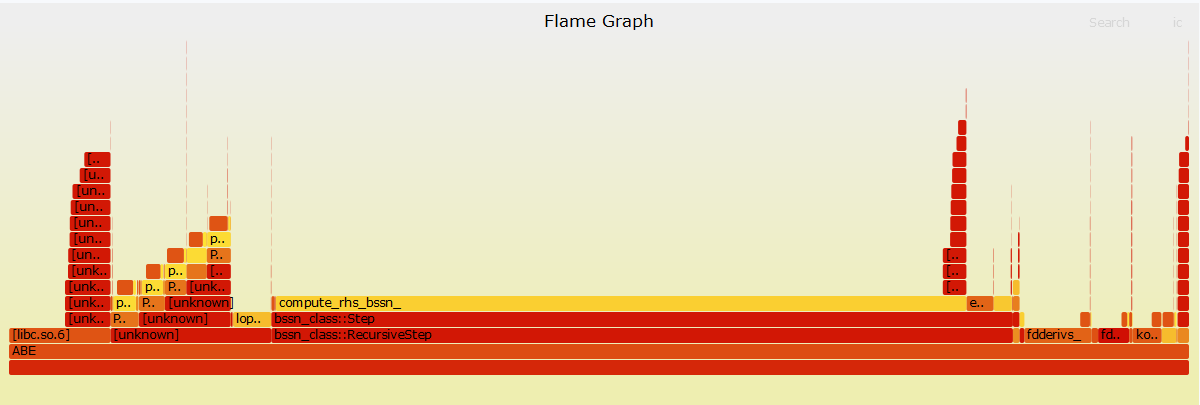
\includegraphics[width=0.8\linewidth]{3.png}
    \caption{FlameGraph before optimization}
    \label{fig:enter-label}
\end{figure}
\begin{figure}
    \centering
    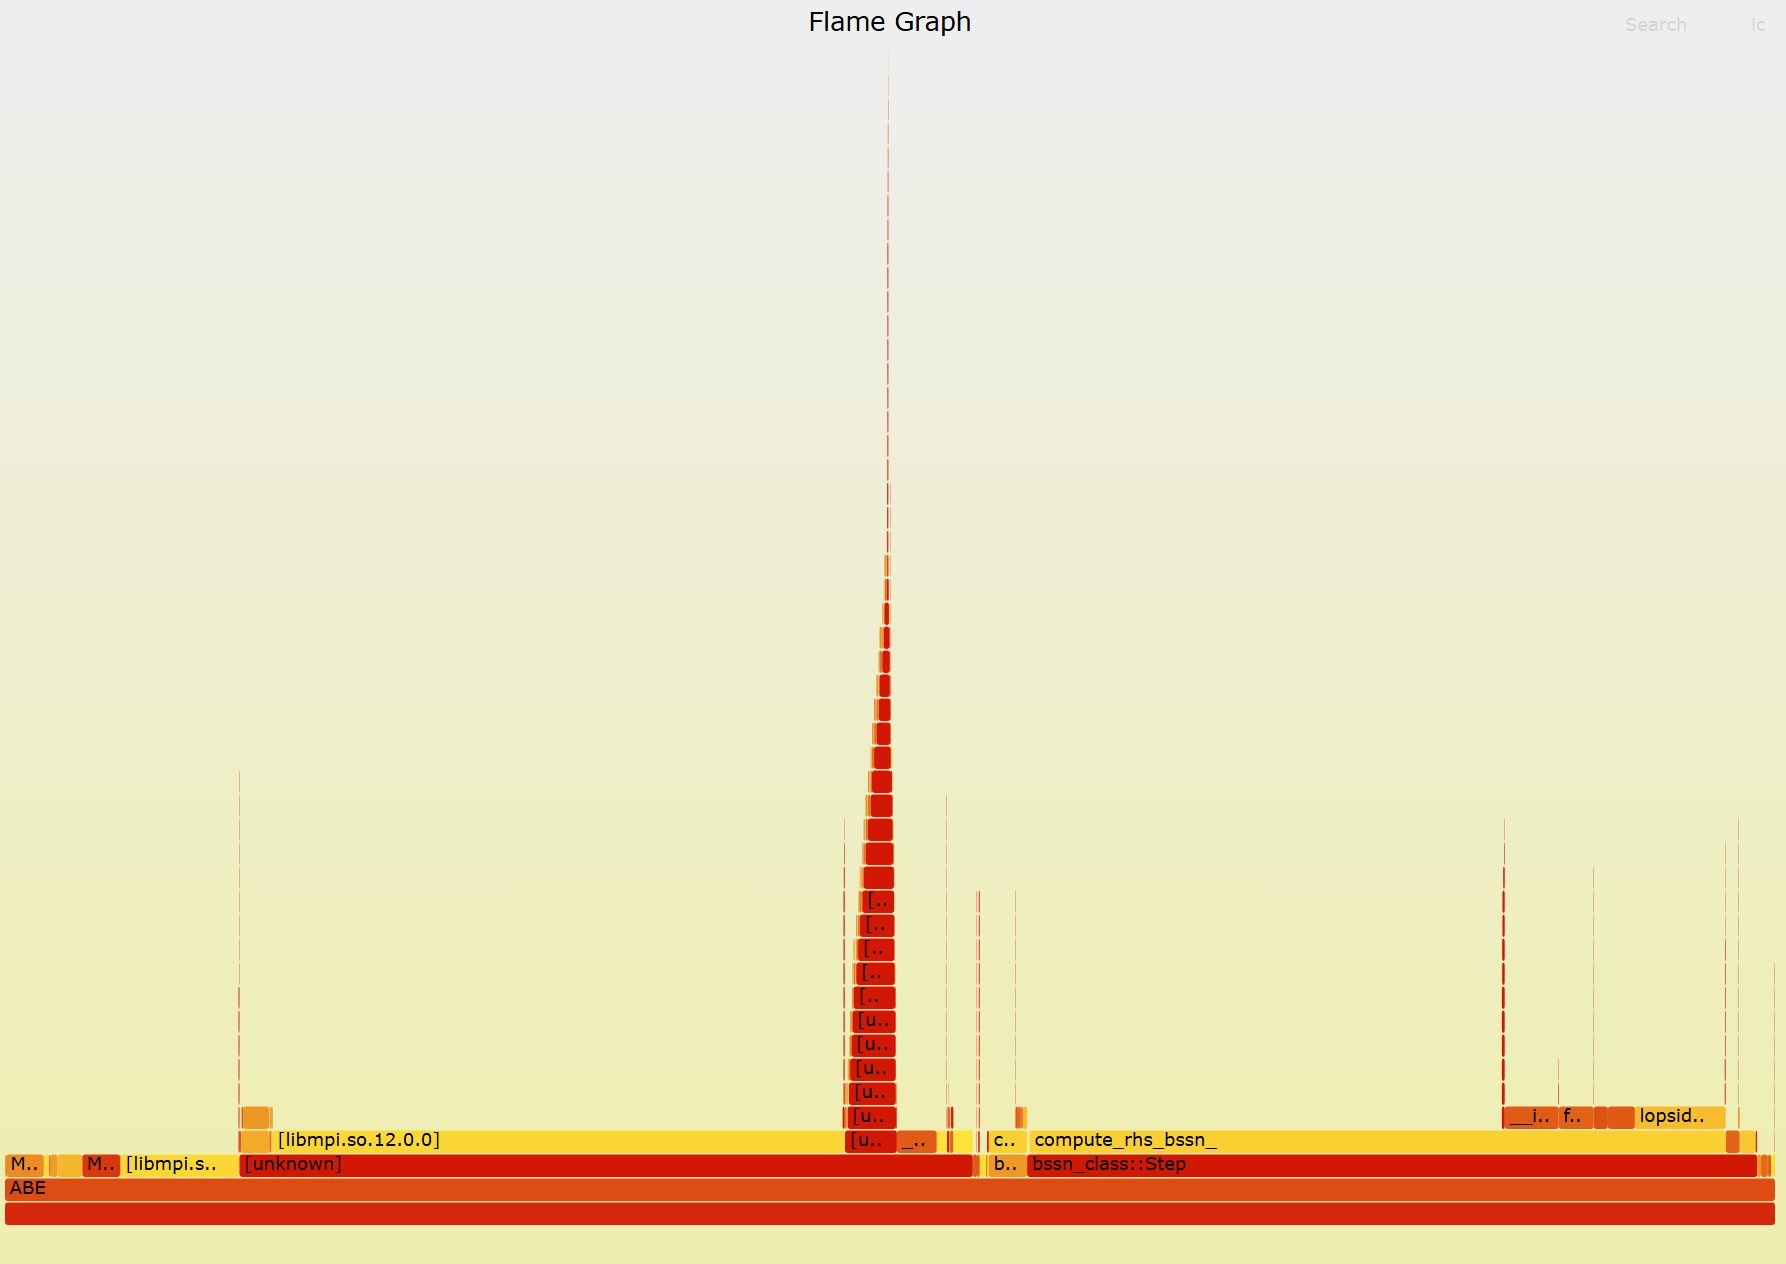
\includegraphics[width=0.8\linewidth]{4.png}
    \caption{FlameGraph after optimization}
    \label{fig:enter-label}
\end{figure}

During AMR evolution, moving refined grids may cause workload imbalance across MPI processes, which increases synchronization wait time and reduces parallel efficiency. To address this, we plan to apply Dynamic Load Balancing (DLB): process workloads will be monitored periodically, and repartitioning will be triggered only when imbalance is significant.

The imbalance is measured by
\[
I=\frac{\max_i L_i}{\frac{1}{N}\sum_{i=1}^{N}L_i},
\]
where \(L_i\) is the workload of process \(i\), and \(N\) is the number of MPI processes. Repartitioning is activated only if \(I\) exceeds a predefined threshold, so migration overhead remains controlled.

We plan to use a Hilbert space-filling curve (Hilbert SFC) for partitioning, as it improves both load balance and spatial locality, thereby reducing communication overhead and improving long-term AMR performance without modifying the physical model.



%#### fortran 代码层面，我们除了编译器flag,还可以在源码中使用编译器指令如：!Intel Fortran Compiler Directive
% !DIR$ ATTRIBUTES ALIGN : 64 :: my_array
%  real(kind=8), allocatable :: my_array(:)
\subsubsection{Hybrid MPI+OpenMP Parallelization Plan}
\ 

In addition to dynamic load balancing, we plan to transition from a pure-MPI model to a hybrid MPI+OpenMP model to improve node-level
resource utilization on multi-core CPUs. The central idea is to reduce the number of MPI ranks per
node while introducing OpenMP threads for intra-rank parallelism in compute-intensive loops
(e.g., stencil updates and local reductions). This strategy is expected to reduce communication
pressure, alleviate synchronization overhead, and improve memory locality through shared-memory
execution within each rank.
The implementation will be incremental: first, identify thread-safe kernels and add OpenMP pragmas in hotspot regions; second, tune rank-thread configurations and affinity policies; third, validate
numerical consistency against the baseline and measure scalability under both strong and weak
scaling settings. The final objective is to improve long-run throughput and parallel efficiency while
preserving physical correctness.

% #### 



\subsection{Conclusion}
\ 
% 1. 总结概述与瓶颈回顾
% 意图：回顾本项目针对 AMSS-NCKU 数值相对论代码的双黑洞合并模拟所进行的系统性优化。明确点出通过性能分析（Profiling）确定的核心瓶颈：3D Stencil 访存受限、冗余指令开销以及 MPI 通信延迟。

% 2. 优化策略大串联
% 意图：高度精炼地总结实施的多层次优化策略。
% 涵盖内容：
% - 编译与架构层：Intel 工具链、AVX2、IPO、64 字节对齐。
% - 算法与代码层：循环融合（Loop Fusion）、消除冗余 Ghost 拷贝、缓存分块（Tiling）提升 L1/L3 利用率。
% - 通信与工程层：全异步非阻塞 MPI 机制实现计算与通信重叠，以及引入 ccache 加速构建。

% 3. 成果重申 (The Punchline)
% 意图：在确保物理和数学正确性（呼应前面的 NaN Check 和 Constraint 检查）的前提下，重申 33.21 小时到 22.38 小时的跨越，以及 1.48 倍的最终加速比。

% 4. 展望未来 (Future Work)
% 意图：完美衔接 Optimization Plans。提出下一步的探索方向（动态负载均衡、代码级别的内存对齐强化如 _mm_malloc 和 Fortran 指令、MPI+OpenMP 混合并行），展现对超算项目长期迭代的工程视野。

In this project, we systematically optimized the AMSS-NCKU numerical relativity code to accelerate high-fidelity Binary Black Hole (BBH) simulations. 
Through rigorous profiling, we identified critical bottlenecks: memory-bound 3D stencil operations, redundant instruction overhead, and MPI communication latency.

To address these, we applied a comprehensive, multi-tiered optimization strategy. 
At the compiler level, we leveraged the Intel toolchain with AVX2 vectorization, IPO, and strict 64-byte memory alignment. 
Algorithmically, we enhanced L1/L3 cache utilization via loop fusion, redundant ghost copy removal, and cache blocking (tiling). 
Furthermore, we overhauled synchronization using fully asynchronous, non-blocking MPI to overlap computation and communication, while integrating \texttt{ccache} to streamline compilation. 
Together, these enhancements reduced the estimated wall-clock time from 33.21 to 21.157 hours, delivering a projected speedup of $\mathbf{1.539\times}$ while preserving strict physical and numerical correctness.

Moving forward, our collaborative efforts will focus on unlocking deeper architectural performance. 
Our primary objectives include implementing dynamic load balancing, enforcing comprehensive code-level memory alignment (e.g., via \texttt{\_mm\_malloc} and Fortran directives), and transitioning to a hybrid MPI+OpenMP parallelization model. 
These continuous improvements will further maximize hardware utilization and push the scaling boundaries of large-scale simulations.

%In this project, we performed a systematic performance study of the AMSS-NCKU numerical relativity code for Binary Black Hole (BBH) simulations and implemented targeted optimizations on the dominant bottlenecks.
%The combined optimizations reduced the estimated wall-clock time from 33.21 hours to 22.38 hours, corresponding to a projected speedup of 1.48×, while preserving physical and numerical correctness.
%Overall, the results confirm that coordinated improvements across compilation, kernel execution, memory locality, and communication are effective for this workload. Future work will focus on dynamic load balancing, broader memory-alignment coverage, and hybrid MPI+OpenMP parallelization to further improve scalability and long-run efficiency.
\newpage

\section*{Acknowledge}
First of all, we would like to express our gratitude to the organizing committee for giving us the opportunity to participate in this competition. 
Secondly, we are grateful to the Computer College of Xiangtan University for providing a comfortable environment during the competition. 
We are also thankful to the High Performance Computing Platform of Xiangtan University. 
We are grateful to our advisor, Peiying Lin, for her strong support throughout the competition. 
We are also very grateful to all the teachers and previous participants who answered our questions and provided us with great assistance.




\clearpage

\bibliographystyle{IEEEtran}
\bibliography{main-blx}
\end{document}
